% Dokumentklassen sættes til memoir.
% Manual: http://ctan.org/tex-archive/macros/latex/contrib/memoir/memman.pdf
\documentclass[a4paper,11pt,twoside,openright,article]{memoir}
\setlrmarginsandblock{*}{2.5cm}{0.75} % højre og venstre 
\setulmarginsandblock{3cm}{*}{1.2} % top og bund 
\checkandfixthelayout[nearest] % specifikt valg af højde algoritme
 
% Danske udtryk (fx figur og tabel) samt dansk orddeling og fonte med
% danske tegn. Hvis LaTeX brokker sig over æ, ø og å skal du udskifte
% "utf8" med "latin1" eller "applemac". 
\usepackage[utf8]{inputenc}
\usepackage[danish]{babel}
\usepackage[T1]{fontenc}
\usepackage{mflogo}

%sexy pdf'er
%\usepackage[export]{adjustbox}
\usepackage{pdfpages}
\usepackage{pdflscape}

%Kompakte lister
\usepackage{paralist}
 
% Matematisk udtryk, fede symboler, theoremer og fancy ting (fx kædebrøker)
\usepackage{amsmath,amssymb}
\usepackage{bm}
\usepackage{amsthm}
\usepackage{mathtools}
\parindent=0pt 

% Fancy ting med enheder og datatabeller. Læs manualen til pakken
% Manual: http://www.ctan.org/tex-archive/macros/latex/contrib/siunitx/siunitx.pdf
\usepackage{siunitx}
 
%Fancy headers, 
%Manual: https://www.sharelatex.com/learn/Headers_and_footers
\let\footruleskip\undefined
\usepackage{fancyhdr}
\pagestyle{fancy}

 
% Indsættelse af grafik. og man kan rotere tekst in line
\usepackage{graphicx} 
\usepackage{fix-cm} 
\usepackage{soul}
\sodef\an{}{0.13em}{0em}{0em} \sodef\ann{}{0.13em}{0.5em}{0em}
 
%Fancy tabeller.
%\usepackage[table]{xcolor}
\usepackage{multirow}
\usepackage{rotating} %sidewaystables!
\usepackage{longtable} %tables spanning multible pages.
\usepackage{tablefootnote} %for at indstætte fornoter i tabeller.
\usepackage{hhline} %Fixer farvede felter
\usepackage{ltxtable} %Longtabular X
\usepackage{tabularx} %Med dynamisk bredte

%URL fodnoter
\usepackage{url}

% Reaktionsskemaer. Læs manualen for at se eksempler.
% Manual: http://www.ctan.org/tex-archive/macros/latex/contrib/mhchem/mhchem.pdf
\usepackage[version=3]{mhchem}

%Lav chapter clickable og fjern border
\usepackage{hyperref}
\hypersetup{
    colorlinks,
    citecolor=black,
    filecolor=black,
    linkcolor=black,
    urlcolor=black
}

%Table of contents settings
\setsecnumdepth{subsection} % organisational level that receives a numbers
\settocdepth{subsection}   % print table of  for level 3

%Til programkode
\usepackage{listings}
\usepackage{color}

\definecolor{dkgreen}{rgb}{0,0.6,0}
\definecolor{gray}{rgb}{0.5,0.5,0.5}
\definecolor{mauve}{rgb}{0.58,0,0.82}
 
\lstset{ 
  language=C++,                % the language of the code
  basicstyle=\footnotesize,           % the size of the fonts that are used for the code
  numbers=left,                   % where to put the line-numbers
  numberstyle=\tiny\color{gray},  % the style that is used for the line-numbers
  stepnumber=1,                   % the step between two line-numbers. If it's 1, each line 
                                  % will be numbered
  numbersep=5pt,                  % how far the line-numbers are from the code
  backgroundcolor=\color{white},      % choose the background color. You must add \usepackage{color}
  showspaces=false,               % show spaces adding particular underscores
  showstringspaces=false,         % underline spaces within strings
  showtabs=false,                 % show tabs within strings adding particular underscores
  frame=single,                   % adds a frame around the code
  rulecolor=\color{black},        % if not set, the frame-color may be changed on line-breaks within not-black text (e.g. commens (green here))
  tabsize=2,                      % sets default tabsize to 2 spaces
  captionpos=b,                   % sets the caption-position to bottom
  breaklines=true,                % sets automatic line breaking
  breakatwhitespace=false,        % sets if automatic breaks should only happen at whitespace
  title=\lstname,                   % show the filename of files included with \lstinputlisting;
                                  % also try caption instead of title
  keywordstyle=\color{blue},          % keyword style
  commentstyle=\color{dkgreen},       % comment style
  stringstyle=\color{mauve},         % string literal style
  escapeinside={\%*}{*)},            % if you want to add LaTeX within your code
  morekeywords={*,...},               % if you want to add more keywords to the set
  rangeprefix=//----------,			%Used for sexy code includes
  rangesuffix=----------,			%---||---
  includerangemarker=false,			%---||---
  literate=
  {á}{{\'a}}1 {é}{{\'e}}1 {í}{{\'i}}1 {ó}{{\'o}}1 {ú}{{\'u}}1
  {Á}{{\'A}}1 {É}{{\'E}}1 {Í}{{\'I}}1 {Ó}{{\'O}}1 {Ú}{{\'U}}1
  {à}{{\`a}}1 {è}{{\`e}}1 {ì}{{\`i}}1 {ò}{{\`o}}1 {ù}{{\`u}}1
  {À}{{\`A}}1 {È}{{\'E}}1 {Ì}{{\`I}}1 {Ò}{{\`O}}1 {Ù}{{\`U}}1
  {ä}{{\"a}}1 {ë}{{\"e}}1 {ï}{{\"i}}1 {ö}{{\"o}}1 {ü}{{\"u}}1
  {Ä}{{\"A}}1 {Ë}{{\"E}}1 {Ï}{{\"I}}1 {Ö}{{\"O}}1 {Ü}{{\"U}}1
  {â}{{\^a}}1 {ê}{{\^e}}1 {î}{{\^i}}1 {ô}{{\^o}}1 {û}{{\^u}}1
  {Â}{{\^A}}1 {Ê}{{\^E}}1 {Î}{{\^I}}1 {Ô}{{\^O}}1 {Û}{{\^U}}1
  {œ}{{\oe}}1 {Œ}{{\OE}}1 {æ}{{\ae}}1 {Æ}{{\AE}}1 {ß}{{\ss}}1
  {ç}{{\c c}}1 {Ç}{{\c C}}1 {ø}{{\o}}1 {å}{{\r a}}1 {Å}{{\r A}}1
  {€}{{\EUR}}1 {£}{{\pounds}}1
}

%Til at udregne forskel mellem sider, brug \pagedifference{A}{B} mellem to labels A og B.
\usepackage{refcount}
\newcommand{\pagedifference}[2]{%
  \number\numexpr\getpagerefnumber{#2}-\getpagerefnumber{#1}\relax}
 
%Til at lave referencer med:
\usepackage{cite}

%Til at lave eksterne \ref til \labels
\usepackage{xr}

%Til at lave \Beam (DC symbol)
\usepackage{marvosym}

%Forsøg på nice lister i tabeller
\usepackage[shortlabels]{enumitem}

\newenvironment{packed_enum}{
\begin{enumerate}[1., topsep=0pt, nosep, partopsep=0pt, itemsep=0pt, parsep=0pt]
}{\end{enumerate}}

\newenvironment{packed_item}{
\begin{itemize}[•, topsep=0pt, nosep, partopsep=0pt, itemsep=0pt, parsep=0pt]
}{\end{itemize}}

%Lækker kommando til at skrive I2C flot uden at bruge \textsuperscript hver gang:
\newcommand*{\IIC}{\texorpdfstring{I\textsuperscript{2}C }{I2C }}

%Lorem ipsum
\usepackage{lipsum}


\usepackage{longtable}
\usepackage{array} % for extrarowheight

%Juicy columntypes - http://tex.stackexchange.com/questions/12703/how-to-create-fixed-width-table-columns-with-text-raggedright-centered-raggedlef
\newcolumntype{L}[1]{>{\raggedright\let\newline\\\arraybackslash\hspace{0pt}}p{#1}}
\newcolumntype{C}[1]{>{\centering\let\newline\\\arraybackslash\hspace{0pt}}p{#1}}
\newcolumntype{R}[1]{>{\raggedleft\let\newline\\\arraybackslash\hspace{0pt}}p{#1}}
\newcolumntype{Z}{>{\raggedright\arraybackslash}X}

%Dejlig kommando til at få nye kapitler på højre side
\newcommand*\cleartorightpage{%
	\clearpage
 	\checkoddpage
	\ifoddpage
  		%do nothing
	\else
		\thispagestyle{empty}
		\mbox{}
 		\clearpage
	\fi
}


%Hacky løsning til at ordne indholdsfortegnelsen.. Why memoir class.. WHY??!
\renewcommand*{\cftdotsep}{1}
\setpnumwidth{3em}
\setrmarg{4em}

%Bugfix til Longtables
\makeatletter
\def\LT@start{%
  \let\LT@start\endgraf
  \endgraf\penalty\z@\vskip\LTpre
  \dimen@\pagetotal
  \advance\dimen@ \ht\ifvoid\LT@firsthead\LT@head\else\LT@firsthead\fi
  \advance\dimen@ \dp\ifvoid\LT@firsthead\LT@head\else\LT@firsthead\fi
  \advance\dimen@ \ht\LT@foot
  \edef\restore@vbadness{\vbadness\the\vbadness\relax}% (added)
  \vbadness=\@M % (added)
  \dimen@ii\vfuzz
  \vfuzz\maxdimen
    \setbox\tw@\copy\z@
    \setbox\tw@\vsplit\tw@ to \ht\@arstrutbox
    \setbox\tw@\vbox{\unvbox\tw@}%
  \vfuzz\dimen@ii
  \restore@vbadness % (added)
  \advance\dimen@ \ht
        \ifdim\ht\@arstrutbox>\ht\tw@\@arstrutbox\else\tw@\fi
  \advance\dimen@\dp
        \ifdim\dp\@arstrutbox>\dp\tw@\@arstrutbox\else\tw@\fi
  \advance\dimen@ -\pagegoal
  \ifdim \dimen@>\z@\vfil\break\fi
      \global\@colroom\@colht
  \ifvoid\LT@foot\else
    \advance\vsize-\ht\LT@foot
    \global\advance\@colroom-\ht\LT@foot
    \dimen@\pagegoal\advance\dimen@-\ht\LT@foot\pagegoal\dimen@
    \maxdepth\z@
  \fi
  \ifvoid\LT@firsthead\copy\LT@head\else\box\LT@firsthead\fi\nobreak
  \output{\LT@output}%
}
\makeatother

\title{Projektdokumentation \\ AutoGreen \\ Gruppe 9}
\author{ 3. Semesterprojekt E3PRJ3-02 \\ Ingeniørhøjskolen, Aarhus Universitet \\ Vejleder: Tore Arne Skogberg}
\date{\today}

\fancyhf{}
\fancyhead[LE,RO]{Gruppe 9 - ''AutoGreen''}
\fancyhead[CE,CO]{Projektdokumentation}
\fancyhead[RE,LO]{IHA, AU}
\fancyfoot[CE,CO]{\leftmark}
\fancyfoot[RE,LO]{\thepage} 

\begin{document}
\frontmatter
\maketitle

\vfill

\begin{table} [h]
	\centering
	\begin{tabular}{|l|r|l|}
	\hline 
	\textbf{Navn} & \textbf{Studienummer} & \textbf{Underskrift~~~~~~~~~~~~~~~~~~~~} \\ \hline
	Morten Hasseriis Gormsen & 201370948 & \\ && \\ \hline
	Kristian Thomsen & 201311478 & \\ && \\ \hline
	Philip Krogh-Pedersen & 201311473 & \\ && \\ \hline
	Lasse Barner Sivertsen & 201371048 & \\ && \\ \hline
	Henrik Bagger Jensen & 201304157 & \\ && \\ \hline
	David Erik Jensen & 11229 & \\ && \\ \hline
	Kasper Torp Samuelsen & 201311498 & \\ && \\ \hline
	Kristian Søgaard Sørensen & 20115255 & \\ && \\ \hline
	\end{tabular}
\end{table}

\clearpage

\setcounter{page}{1}
\thispagestyle{plain}
\tableofcontents
\thispagestyle{plain}

\chapter*{Forfattere} %TODO Alle afsnit skal skrives ind her!
\begin{table}[h]
\centering
\begin{tabularx}{\textwidth * 5/6}{|l|X|}
	\hline
	Afsnit & Forfatter(e) \\ \hline
	\ref{ch:Projektformulering} \nameref{ch:Projektformulering} & Alle \\ \hline
	\ref{ch:Kravspec} \nameref{ch:Kravspec} & Alle \\ \hline
	\ref{ch:Accepttest} \nameref{ch:Accepttest} & Alle \\ \hline
	\ref{ch:SysArk} \nameref{ch:SysArk} & Alle \\ \hline
	\ref{ch:HwDesign} \nameref{ch:HwDesign} & Kristian T, Philip, Lasse, Henrik og Morten \\ \hline
 		\ref{sec:PSoC_Master_impl} \nameref{sec:PSoC_Master_impl}  & Philip, Lasse og Kristian T \\ \hline
		\ref{sec:AktImpl} \nameref{sec:AktImpl} & Henrik og Morten \\ \hline
		\ref{sec:PsuImpl} \nameref{sec:PsuImpl} & Henrik og Morten \\ \hline
\end{tabularx}
\end{table}

\mainmatter
\chapter{Projektformulering} \label{ch:Projektformulering}

\section{Version}
\begin{table}[h]
	\centering
	\begin{tabularx}{\textwidth - 2cm}{|l|l| l|X|}
	\hline
	Dato	& Version	& Initialer & Ændring	\\ \hline
	26. februar & 1 & MHG & Første udkast. \\ \hline
	4. marts & 2 & LBS & Mindre rettelser efter første review. \\ \hline
	12. marts & 3 & MHG & Mindre rettelser efter fælles gennemlæsning. \\\hline
	\end{tabularx}
\end{table}
\section{Beskrivelse}
Mange har prøvet at kaste sig ud i et nyt projekt, som for eksempel at dyrke frugt og grønt i drivhus, men pludselig glemmer man at vande, holde øje med temperaturen og lignende, og så er projektet gået i vasken.
 
AutoGreen hjælper den nye drivhusbruger med at holde styr på basale parametre som temperatur og fugtighed, men det er også for den mere erfarne drivhusbruger, som ønsker optimale forhold i drivhuset, eller som ønsker at vælge de mest egnede planter ud fra de forhold, der er i drivhuset.
 
Ved dyrkning af planter i et drivhus, er temperaturen en af de vanskeligste ting at kontrollere. Man er ikke altid hjemme, når drivhuset skal åbnes og lukkes, hvilket sjældent er samme tid på dagen; det afhænger af udendørstemperatur, skydække mm. 
Der findes mekaniske vinduesåbnere, som åbner og lukker et eller flere vinduer i drivhuset vha. en gasfyldt cylinder. 
Disse er dog forholdsvis upræcise, og reguleringen af temperaturen er langsom. Der er desuden ikke mulighed for at få ekstra varme tilført, hvilket kan være et stort problem, hvis vejret er ustabilt, særligt i starten af sæsonen. 
AutoGreen styrer temperaturen i drivhuset vha. en vinduesåbner, tovejs luftcirkulation og et varmelegeme. 
Dette giver en hurtig og præcis regulering af temperaturen. Varmelegemet tilfører ekstra varme, hvis der er for koldt i drivhuset. 
Dette kan meget vel redde planterne, hvis det viser sig, at man har plantet ud for tidligt, og det giver mulighed for at forspire i drivhuset, selv om drivhussæsonen ikke er startet. 
Hvis der er for varmt i drivhuset, åbner vinduet, og hvis dette ikke er tilstrækkeligt, anvendes også luftcirkulationen til at regulere temperaturen. 
Brugeren har mulighed for at vælge mellem forskellige måder at styre temperaturen på. Ønskes optimale forhold hurtigst muligt døgnet rundt, anvendes både varmelegeme, vinduesåbner og luftcirkulation. 
Brugeren kan også vælge fx at udelade brugen af varmelegemet eller luftcirkulationen, hvis en mere økonomisk temperaturregulering ønskes. 
 
En anden vigtig parameter for drivhusplanternes trivsel er selvfølgelig vanding, hvilket ligesom regulering af temperaturen kan være problematisk, hvis man ikke er hjemme, eller man ganske simpelt glemmer det. 
AutoGreen kan vha. en eller flere fugtmålere i drivhusjorden give brugeren besked om, at det er tid til at vande, ligesom et tilkoblet automatisk vandingssystem kan aktiveres. Et sådant vandingssystem er ikke en del af AutoGreen.
Forskellige planter kræver forskellig mængde vand, og brugeren har derfor mulighed for at bruge op til seks fugtmålere, som kan placeres i jorden ved forskellige plantetyper. 

AutoGreen måler desuden luftfugtighed og lysmængde i drivhuset; disse målinger logges sammen med målinger af fugtighed i jorden og temperaturmålinger. 
Brugeren kan vha. en database med de mest almindelige drivhusplanter vælge, hvad han vil dyrke i sit drivhus, eller han kan forsøge at optimere forholdene i drivhuset, hvis han ønsker bedre forhold for en bestemt type plante.  
Brugeren har mulighed for at tilføje ekstra planter i databasen. 

AutoGreen systemet kontrolleres af brugeren vha. en grafisk brugerflade med touch display, der realiseres på et Embest DevKit8000 Evaluation Board. \cite{lib:DK8000}
Alle sensorer og aktuatorer samt systemets masterenhed realiseres vha. PSoC4 udviklingsboards (CY8CKIT-042). \cite{lib:psoc4_guide}

\clearpage

\section{MoSCoW prioritering}
Ambitionen for dette projekt er som absolut minimum at realisere nedenstående punkter under \textit{"skal"}. 
Det forventes desuden at punkterne under \textit{"bør"} realiseres, men de har lavere prioritet.
Punkterne under \textit{"kan"} forventes ikke realiseret, og punkterne under \textit{"vil ikke..."} realiseres med sikkerhed ikke. 
Sidstnævnte punkter kan ses som udviklingsmuligheder i forhold til senere versioner af systemet. 

\begin{itemize}
	\item \textbf{Systemet skal:}
		\begin{itemize}
			\item Kunne monitorere temperaturen i drivhuset og regulere temperaturen i drivhuset vha. varmelegeme, åbning af vinduer og luftcirkulation.
			\item Give brugeren mulighed for at vælge varmelegeme og/eller luftcirkulation fra, hvis en mere økonomisk regulering af temperaturen ønskes. 
			\item Have et grafisk user interface.
		\end{itemize}
	\item \textbf{Systemet bør:}
		\begin{itemize}
			\item Måle jordfugtighed med op til seks sensorer i drivhuset og give brugeren besked på displayet om, at det er tid til at vande. 
			\item Måle Lysintensitet og luftfugtihed i drivhuset.
			\item Indeholde en log over alle målte parametre; jordfugtighed, temperatur, luftfugtighed og lysmængde. 
			Dataene præsenteres grafisk for brugeren.
			\item Indeholde en database over de mest almindelige drivhusplanter, så brugeren kan orientere sig om en plantes optimale forhold.
			\item Indeholde en systemlog, som noterer vigtige system hændelser.
		\end{itemize}
	\item \textbf{Systemet kan:}
		\begin{itemize}
			\item Sende besked til brugeren via email, om at det er tid til at vande.
Tilkobles et automatisk vandingssystem, som aktiveres ved behov for vanding. 
			\item Give brugeren mulighed for at tilføje planter i databasen.
			\item Give brugeren mulighed for at kommunikere trådløst med systemet fra brugerfladen, så denne kan placeres fx inde i brugerens bolig. 
		\end{itemize}
	\item \textbf{Systemet vil ikke i denne version:}	
		\begin{itemize}
			\item Indeholde et kamera, og tilhørende billedarkiv, som giver brugeren mulighed for at følge planternes udvikling fra dag til dag. 
			\item Give brugeren mulighed for at agere med systemet via en app på dennes mobiltelefon. 
		\end{itemize}
\end{itemize}
\clearpage

\section{Rigt Billede}
\begin{figure}[h]
\centering 
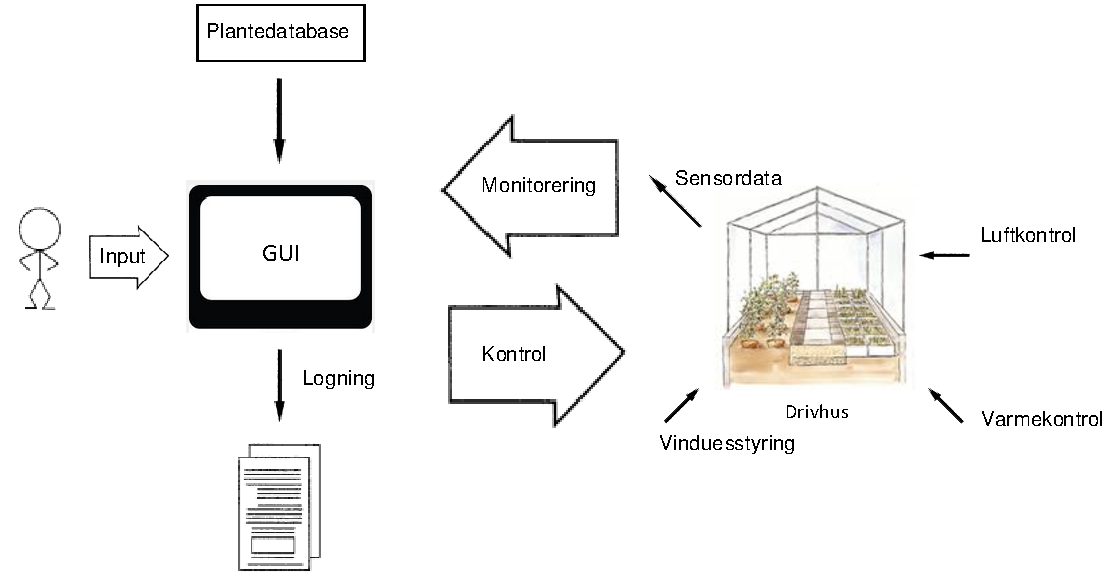
\includegraphics[width={\textwidth}] {../fig/Rigt_Billede.pdf}
\caption{AutoGreen Automatiseret Drivhus}
\label{fig:Rigt_Billede}
\end{figure}

\chapter{Kravspecifikation (Alle)}

\section{Version}
\begin{table}[h]
	\centering
	\begin{tabularx}{\textwidth - 2cm}{|l|l|l|X|}
	\hline
	Dato	& Version	& Initialer & Ændring	\\ \hline
	26. februar & 1 & MHG & Første udkast. \\ \hline
	6. marts & 2 & MHG & Rettelser efter review. \\ \hline
	\end{tabularx}
\end{table}

\section{Systembeskrivelse}

Systemet AutoGreen fungerer som et intelligent drivhus, med hovedformålene at kunne monitorere og regulere nogle forskellige parametre i drivhusets indre. Blandt parametrene vil der være jordfugt-, luftfugt-, temperatur- og lyssensorer og de enheder, som systemet kommer til at bestå af, kan ses på Figur \ref{fig:systemoversigt}. Nogle af parametrene vil desuden kunne reguleres, således det bliver muligt for en bruger at kunne automatisere sit drivhus. Selve drivhuset som projektet drejer sig om, er en mindre model, med dimensioner som set på Figur \ref{fig:dimensioner}. 

\begin{figure}[!h]
\centering 
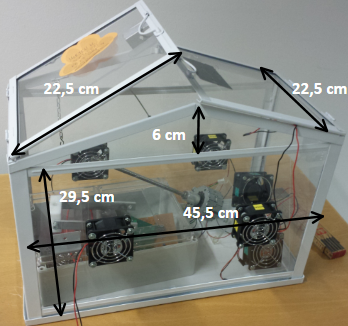
\includegraphics[scale=0.9] {../fig/dimensioner.png}
\caption{Dimensioner for drivhus.}
\label{fig:dimensioner}
\end{figure}

Ud fra billedet ses blæsere samt vinduesmotoren (ej monteret på billedet), som skal regulere temperaturen i drivhuset. Disse indgår som en del af systemet, men selve huset gør ikke. Der vil ydermere være et varmelegeme, som ikke er repræsenteret på billedet. 

\subsubsection{DevKit8000}
DevKit8000 er systemets kontrolenhed og brugergrænseflade. 
DevKit8000 modtager input fra brugeren på dens touch skærm, og den kan give output til brugeren på skærmen og via e-mail; den er koblet til internet via ethernet. 
DevKit8000 kan desuden måle og regulere klimaet i det fysiske drivhus; det sker vha. en \IIC Master, hvortil der kommunikeres vha. UART.
\subsubsection{\IIC Master}
I\textsuperscript{2}C Master er realiseret på et PSoC4 udviklingsboard (CY8CKIT-042). 
\IIC Master modtager input fra DevKit8000 og sender/modtager data til/fra \IIC Slaver, hvorefter respons sendes retur til DevKit8000.	
\subsubsection{\IIC Slave Temperatur}
\IIC Slave Temperatur er ansvarlig for alle handlinger og målinger, der har med temperaturen i det fysiske drivhus at gøre. Der er tilkoblet en temperatursensor og tre aktuatorer, hhv. vinduesåbner, blæsere og varmelegeme. 
Enheden er realiseret på et PSoC4 udviklingsboard (CY8CKIT-042).
\subsubsection{\IIC Slave Jordfugtighed}
\IIC Slave Jordfugtighed er ansvarlig for alle handlinger og målinger, der har at gøre med vanding i det fysiske drivhus. Der kan tilkobles 0 - 6 jordfugtighedssensorer med tilhørende aktuator til et evt. vandingssystem. Selve vandingssystemet er ikke en del af AutoGreen, en vandingsaktuator er en high/low bool. Enheden er realiseret på et PSoC4 udviklingsboard (CY8CKIT-042).
\subsubsection{\IIC Slave Luftfugtighed/Lys}
\IIC Slave Luftfugtighed/Lys er ansvarlig for måling af lysintensitet og luftfugtighed i det fysiske drivhus. Enheden er realiseret på et PSoC4 udviklingsboard (CY8CKIT-042).

\clearpage

\begin{figure}[!h]
\centering 
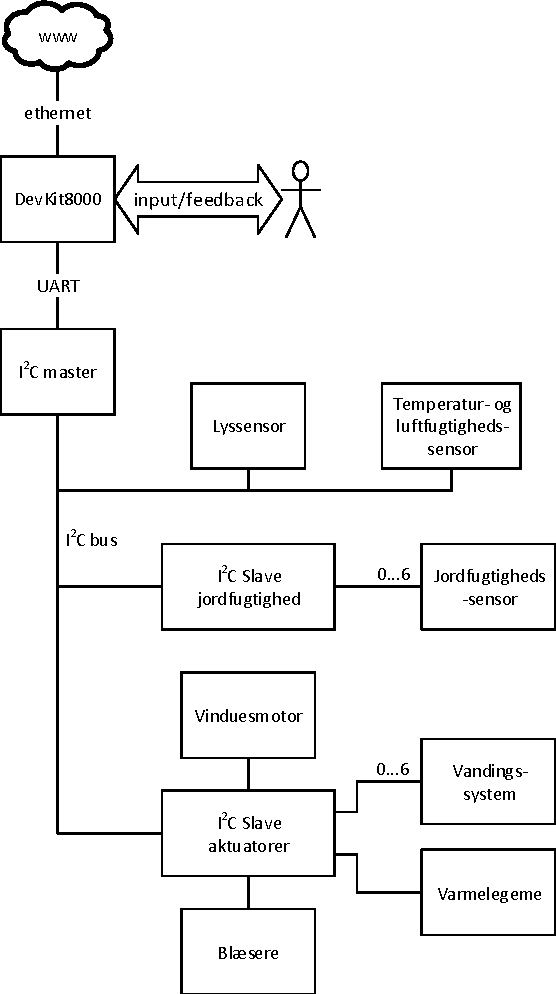
\includegraphics[height={\textheight - 2 cm}, trim=0 0 0 0, clip=true] {../fig/systemoversigt/sys_fig.pdf}
\caption{Oversigt over system}
\label{fig:systemoversigt}
\end{figure}

\clearpage

\section{Ordforklaring}

\subsubsection{Plantedatabase}
Plantedatabasen indeholder information om ideelle forhold for forskellige typer planter, som brugeren kunne tænkes at plante i sit fysiske drivhus. 
Informationen i plantedatabasen står til grund for udgangsparametre for nye planter i det virtuelle drivhus. Der findes en række systemplanter, som brugeren ikke kan redigere eller slette, men brugeren kan tilføje egne planter.
\subsubsection{Data Log}
Systemet er udstyret med en log over de indsamlede data fra sensorer i systemet, der måles og indskrives i loggen hvert minut. 
Denne er opbygget som en database, hvor hver logning indeholder information fra de diskrete sensorer samt et tidspunkt. 
\subsubsection{System Log}
Systemet er udstyret med en log over hvad systemet foretager sig. 
Dette kunne f.eks. være et indlæg når systemet foretager en måling, sender en e-mail, regulerer miljøet i drivhuset.
\subsubsection{Virtuelt Drivhus}
Det virtuelle drivhus er oversigten over planter samt information omkring miljø, som brugeren kan se i selve systemet. 
\subsubsection{Fysisk Drivhus}
Ved det fysiske drivhus forstås det drivhus hvori systemet er monteret. 
Det virtuelle drivhus skal så vidt muligt afspejle det fysiske drivhus, hvor brugeren har sine planter.
\subsubsection{Konfigurationsfil}
Dette er en automatisk genereret fil, der er placeret på dev-kittet, som indeholder brugerens konfigurationer om blandt andet notifikationer, e-mailadresser, antallet af fugtsensorer og deres unikke id mm.

\clearpage

\section{Brugerfladen}

I Figur \ref{fig:gui_skitse} er vist en skitse over hvordan brugerfladen forventes at se ud. De grå områder uner Hovedmenu er knapper, brugeren kan trykke på for at tilgå yderligere menuer. Nederst ses "Monitorer" og "Reguler" knapper, som kan aktivere eller deaktivere hhv. monitorerings- og reguleringsfunktionalitet. Til højre ses live status for det fysiske drivhus, samt live status for jordfugtighed for hver plante i bunden. I bunden af billedet til højre, kan der ses nogle knapper i forskellige farver. Disse symboliserer planter i det virtuelle drivhus, og forklarer tilfældet for den enkelte plante. Grøn betyder at plantens jordfugtighed er indenfor tolerancerne, hvor rød betyder det modsatte. Grå (Not Available) betyder at der ikke er placeret en plante i det virtuelle drivhus, for den pågældende fugtighedssensor. 

\begin{figure}[h]
\centering
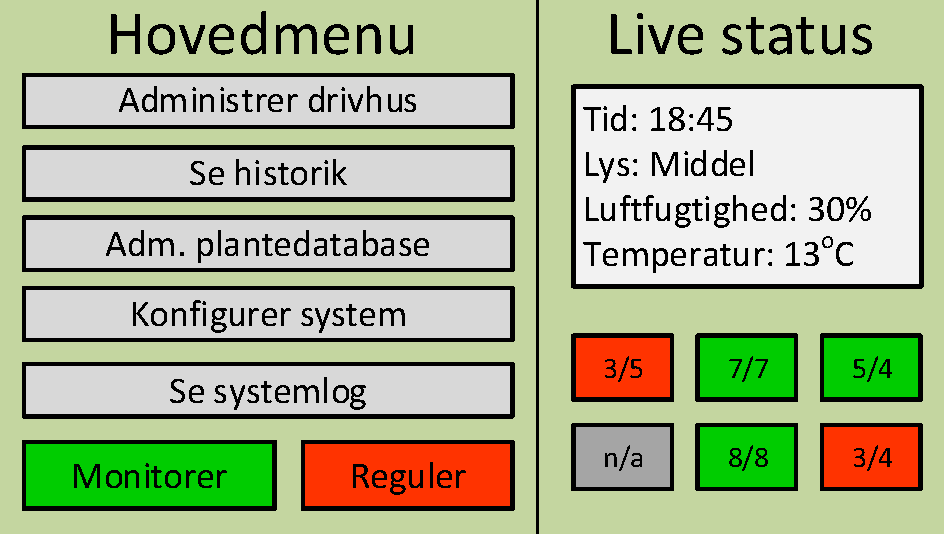
\includegraphics[width=\textwidth - 3 cm]{../fig/gui_skitse}
\caption{Skitse af hovedmenuen på brugerfladen.}
\label{fig:gui_skitse}
\end{figure}

\clearpage

\section{Aktør Kontekst Diagram} 
\begin{figure}[h]
\centering 
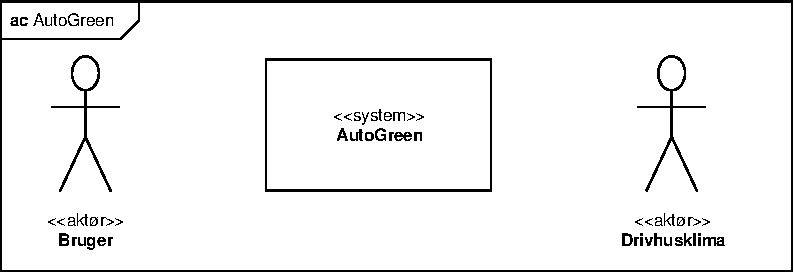
\includegraphics[width={\textwidth}, trim=0 0 0 0, clip=true] {../fig/Aktoer_Kontekst_Diagram.pdf}
\caption{Aktør Kontekst Diagram for AutoGreen}
\label{fig:aktoer_kontekst_diagram}
\end{figure}

\subsection{Aktørbeskrivelser}

\subsubsection{Bruger - Primær Aktør}
Brugeren kan:
\begin{itemize}
\item Starte og stoppe systemet 
\item Overvåge det aktuelle klima i drivhuset. 
\item Administrere drivhuset, hvilket vil sige at han giver systemet input om hvilke planter der er i drivhuset. 
\item Se historik over klimaet i drivhuset
\item Konfigurere systemindstillinger
\item Se systemlog
\item Modtage rapportering om klimaet i drivhuset 
\end{itemize}

\subsubsection{Drivhusklima - Sekundær Aktør}
Drivhusklimaet består af en række parametre, som systemet måler og/eller regulerer:
\begin{itemize}
\item Lufttemperatur
	\subitem Måles, registreres og reguleres af systemet
\item Jordfugtighed
	\subitem Måles, registreres og reguleres indirekte af systemet
\item Luftfugtighed
	\subitem Måles og registreres af systemet
\item Lysintensitet
	\subitem Måles og registreres af systemet
\end{itemize}

\section{Funktionelle Krav}
Systemet\ldots
\begin{enumerate}\itemsep1pt \parskip0pt \parsep0pt
	\item \ldots \emph{Skal} give brugeren mulighed for at monitorere og konfigurere drivhusklimaet vha. en grafisk brugerflade på et touch display.
	\item \ldots \emph{Skal} have mulighed for at starte og stoppe systemet.
	\item \ldots \emph{Skal} måle lufttemperatur i det fysiske drivhus.
	\item \ldots \emph{Skal} kunne regulere temperatur i det fysiske drivhus.
	\item \ldots \emph{Skal} kunne indstilles til brugerdefineret tid og dato.
	\item \ldots \emph{Skal} kunne give brugeren mulighed for at vælge brug af varmelegeme og ventilatorer.
	\item \ldots \emph{Skal} give brugeren mulighed for at tilføje en plante i det virtuelle drivhus.
	\item \ldots \emph{Skal} give brugeren mulighed for at fjerne en plante i det virtuelle drivhus.
	\item \ldots \emph{Skal} give brugeren mulighed for at redigere en plante i det virtuelle drivhus.
	\item \ldots \emph{Skal} kunne regulere drivhusklima automatisk efter behov.
	\item \ldots \emph{Bør} kunne måle jordfugtighed i fysiske drivhus.
	\item \ldots \emph{Bør} kunne måle lysintensitet i det fysiske drivhus.
	\item \ldots \emph{Bør} kunne måle luftfugtighed i det fysiske drivhus.
	\item \ldots \emph{Bør} indeholde informationer om planter i en datastruktur.
	\item \ldots \emph{Bør} kunne fremvise grafisk historik over måledata fra drivhus.
	\item \ldots \emph{Bør} kunne vise planteinformationer fra plantedatabasen.
	\item \ldots \emph{Bør} give brugeren mulighed for at se en systemlog over hændelser i systemet.
	\item \ldots \emph{Bør} gemme alt monitorering i en data log.
	\item \ldots \emph{Kan} give brugeren mulighed for at redigere og slette planter i plantedatabasen, som brugeren selv har tilføjet.
	\item \ldots \emph{Kan} give brugeren mulighed for at tilføje/redigere/slette e-mail adresser.
	\item \ldots \emph{Kan} give brugeren mulighed for valg af varslingse-mail omhandlende dårligt klima og daglig e-mail.
	\item \ldots \emph{Kan} sende e-mail til brugeren, på baggrund af brugerindstillinger.
\end{enumerate}

\section{Ikke Funktionelle Krav}
Systemet\ldots
\begin{enumerate}\itemsep1pt \parskip0pt \parsep0pt
	\item \ldots \emph{Skal} minimum måle parametre i det fysiske drivhus med 1 minuts mellemrum +/- 5 sekunder.
	\item \ldots \emph{Skal} kunne justere temperaturen i det fysiske drivhus til det ønskede niveau på højst 30 minutter ved en starttemperatur der ligger højst 10 grader fra det ønskede niveau, når alle tre aktuatorer anvendes.
	\item \ldots \emph{Skal} kunne måle jordfugtighed i trin á 10, hvor 10 er mest fugtigt. 
	\item \ldots \emph{Skal} kunne indeholde op til seks fugtmålere.
	\item \ldots \emph{Skal} anvende DevKit8000 med indlejret Linux platform.
	\item \ldots \emph{Skal} anvende mindst et PSOC 4 udviklingsboard.
	\item \ldots \emph{Skal} kunne indeholde op til 100 planter i plantedatabasen.
	\item \ldots \emph{Skal} kunne indeholde data et år tilbage i tiden.
	\item \ldots \emph{Skal} kunne måle temperaturen med en præcision på +/- 1 grad celcius ved 20 grader.
	\item \ldots \emph{Skal} kunne indeholde op til tre e-mail adresser.
	\item \ldots \emph{Bør} kunne justere temperaturen til 25 grader celcius i det fysiske drivhus med en præcision på +/- 2 grad, når drivhuset er placeret i et rum ved stuetemperatur (ca. 20 grader).
	\item \ldots \emph{Kan} sende mail til brugeren højest 1 minut efter et for lavt jordfugtighedsniveau er målt, hvis den er indstillet til dette.
\end{enumerate}


\section{Use Case Diagram}
\begin{figure}[h]
\centering 
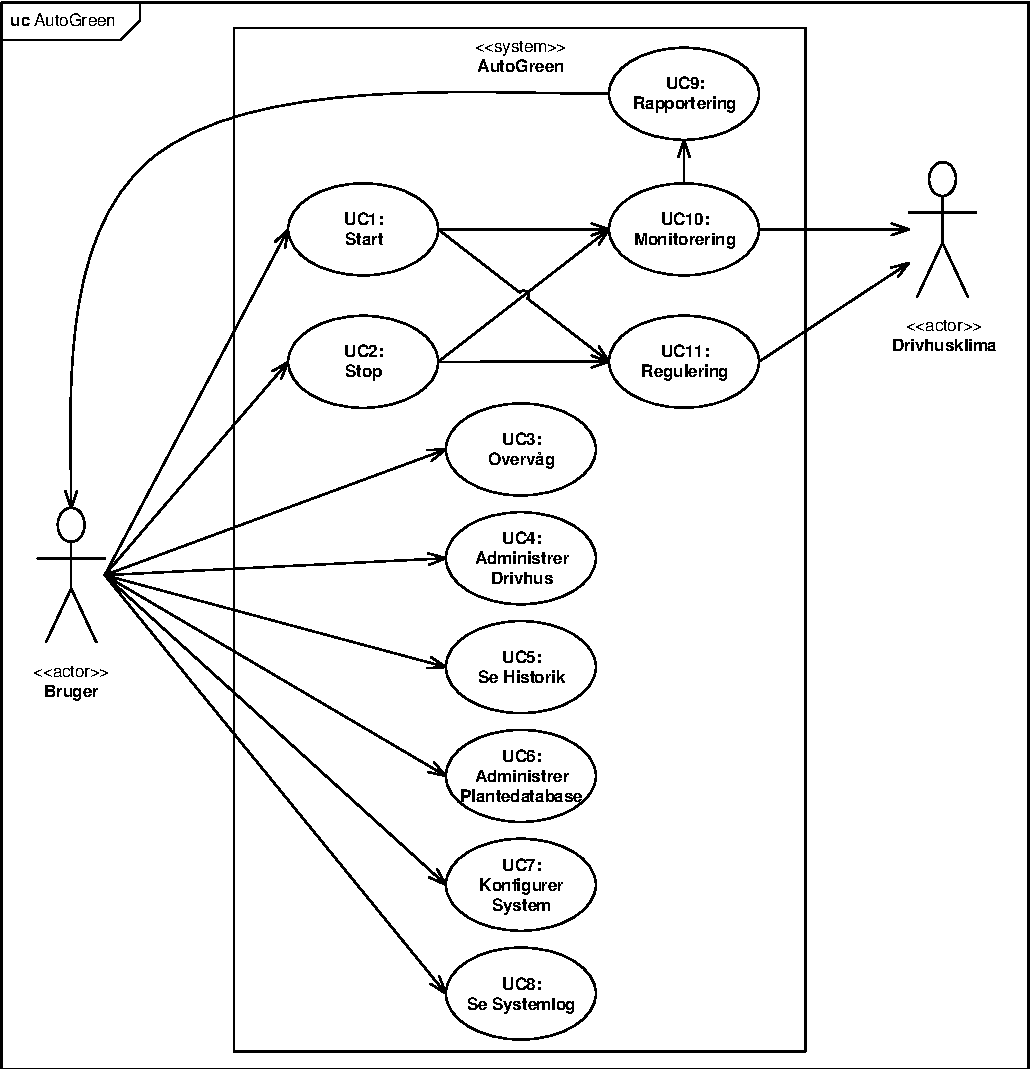
\includegraphics[width={\textwidth-1cm}, trim=0 0 0 0, clip=true] {../fig/UC_Diagram.pdf}
\caption{Use Case Diagram for AutoGreen}
\label{fig:use_case_diagram}
\end{figure}

\clearpage

\subsection{Use Case beskrivelser - Initiering og Formål}
\subsubsection{UC1: Start}
Initieres af: Bruger

Denne UC giver brugeren mulighed for at starte systemet, dvs. monitorering og regulering af drivhusklimaet. 
Brugeren har mulighed for kun at starte monitorering. Use Case’en kan initiere UC10 Rapportering og UC11 Monitorering.

\subsubsection{UC2: Stop}
Initieres af: Bruger

Denne UC giver brugeren mulighed for at stoppe systemet, dvs. monitorering og regulering af drivhusklimaet. 
Brugeren har mulighed for kun at stoppe regulering. Use Case’en kan stoppe UC10 Rapportering og UC11 Monitorering.

\subsubsection{UC3: Overvåg}
Initieres af: Bruger

Når monitorering er startet, vises der i user interfacets hovedmenu live opdaterede måleværdier. 
Såfremt UC10 Monitorering er startet, kan værdierne for lufttemperatur og jordfugtighed være røde, hvis de ikke passer med de ønskede værdier.

\subsubsection{UC4: Administrer Drivhus}
Initieres af: Bruger

Denne UC giver brugeren mulighed for at informere systemet om hvilke planter der er i drivhuset. 
Han kan tilføje op til seks planter fra plantedatabasen i drivhuset, og han kan redigere parametre for disse, hvis han ønsker andre parametre end dem der fremgår i plantedatabasen. 
Hver af disse planter kan forbindes med en jordfugtighedsmåler. 

\subsubsection{UC5: Se Historik}
Initieres af: Bruger

Denne Use Case giver brugeren mulighed for at se grafisk historik over de fire målte parametre i drivhuset. 
Brugeren kan se data op til et år tilbage i tiden. 

\subsubsection{UC6: Administrer Plantedatabase}
Initieres af: Bruger

Denne UC giver brugeren mulighed for at se på planter i databasen. 
Han kan desuden tilføje og fjerne egne planter i databasen, og han kan redigere i de planter han tidligere har tilføjet. 
Han kan ikke redigere eller fjerne planter han ikke selv har tilføjet. 

\subsubsection{UC7: Konfigurer System}
Initieres af: Bruger

Denne UC giver brugeren mulighed for at rette i systemindstillinger, herunder:
\begin{itemize}
\item Indstille tid og dato
\item Tilføje/fjerne/rette e-mail adresse 
\item Aktivering/deaktivering af advarsler om dårligt klima sendt pr. mail
\item Aktivering/deaktivering af daglig status sendt pr. mail
\item Aktivering/deaktivering af varmelegeme
\item Aktivering/deakttivering af luftcirkulation
\end{itemize}

\subsubsection{UC8: Se System Log}
Initieres af: Bruger/Tekniker

Denne UC giver brugere eller teknikeren mulighed for at se en liste over systemhændelser, herunder:
\begin{itemize}
\item Start og stop af system
\item Manglende kontakt til sensorer
\item Afsendte e-mails
\item Tilføjede/fjernede/redigerede planter i drivhuset
\item Tilføjede/fjernede/redigerede planter i plantedatabasen
\item Konfigurationsændringer
\item Fejl i registrering i datalog
\item Fejl på vinduesåbner
\item Fejl på Luftcirkulation
\item Fejl på varmelegeme
\end{itemize}

\subsubsection{UC9: Rapportering}
Initieres af: UC10 Monitorering

Denne Use Case rapporterer til brugeren ud fra de indstillinger brugeren har valgt under UC7 Konfigurer System. 
Dette sker ved afsendelse af e-mail til den eller de adresser, som brugeren ligeledes har tilføjet under UC7 Konfigurer System.

\subsubsection{UC10: Monitorering}
Initieres af: UC1 Start.

Denne Use Case lagrer kontinuerligt målinger af lufttemperatur, jordfugtighed, luftfugtighed og lysintensitet i en data log fil. 
Lagringen sker en gang i minuttet. 

\subsubsection{UC11: Regulering}
Initeres af: UC1 Start.

Denne Use Case regulerer temperaturen i drivhuset, som udgangspunkt vha. vinduesåbner, varmelegeme og luftcirkulation. 
Det kan ske uden luftcirkulation og/eller varmelegeme, hvis brugeren har valgt dette under UC7 Konfigurer System. Det er ikke muligt at aktivere regulering uden at UC10 Monitorering er aktiveret.

\clearpage

\subsection{Use Case Beskrivelser - Fully Dressed}
For alle Use Cases hvor brugeren navigerer i undermenuer af hovedmenuen, gælder det, at brugeren har mulighed for at gå et skridt tilbage ved at trykke på en ”tilbage knap”. Fremover ved benævningen ”Systemet er operationelt” menes, at systemet er tilsluttet tilstrækkelig strømforsyning og at alt fungerer efter hensigten og at systemet er tilsluttet ethernet.

%UC1
\begin{table}[h]
\begin{tabularx}{\textwidth}{| >{\raggedright\arraybackslash}p{3.3 cm} | >{\raggedright\arraybackslash}X |} \hline

\textbf{Navn:} 						& UC1: Start\\ \hline
\textbf{Mål:}						& At starte systemet helt eller delvist. \\ \hline
\textbf{Initering:}					& Bruger \\ \hline
\textbf{Aktører:} 					& Bruger (primær) \\ \hline
\textbf{Reference:} 					& UC10: Monitorering, UC11: Regulering \\ \hline
\textbf{Antal samtidige forekomster:} & En \\ \hline
\textbf{Forudsætning:} 				& Systemet er stoppet helt, er operationelt og viser hovedmenuen.\\ \hline
\textbf{Resultat:}					& At systemet er startet helt eller delvist. \\ \hline
\textbf{Hovedscenarie:}				& 

\begin{packed_enum}
\item Bruger trykker på monitorerings knap. 
\item System aktiverer UC10: Monitorering. 
\item Bruger trykker på regulerings knap. 
	\begin{packed_item}\itemsep1pt \parskip0pt \parsep0pt
	\item {[}Ext 3.a : Bruger vælger kun monitorering.{]}
	\end{packed_item}
\item Systemet aktiverer UC11: Regulering.
\end{packed_enum} \\ \hline
\textbf{Udvidelser:}				&  
\textbf{{[}Ext 3.a : Bruger vælger kun monitorering.{]}}
	\begin{packed_enum}\itemsep1pt \parskip0pt \parsep0pt
	\item Systemet fortsætter ved pkt. 5 i hovedscenarie.
	\end{packed_enum}
\\ \hline
\end{tabularx}
\caption{UC1: Start}
\label{tbl:UC1}
\end{table}

\clearpage
%UC2
\begin{table}[h]
\begin{tabularx}{\textwidth}{| >{\raggedright\arraybackslash}p{3.3 cm} | >{\raggedright\arraybackslash}X |} \hline

\textbf{Navn:} 						& UC2: Stop\\ \hline
\textbf{Mål:}						& At stoppe systemet helt eller delvist. \\ \hline
\textbf{Initering:}					& Bruger \\ \hline
\textbf{Aktører:} 					& Bruger (primær) \\ \hline
\textbf{Reference:} 					& UC10: Monitorering, UC11: Regulering \\ \hline
\textbf{Antal samtidige forekomster:} & En \\ \hline
\textbf{Forudsætning:} 				& Både UC10: Monitorering og UC11: Regulering er startet, systemet er operationelt og viser hovedmenuen.\\ \hline
\textbf{Resultat:}					& At systemet er stoppet helt eller delvist. \\ \hline
\textbf{Hovedscenarie:}				& 

\begin{packed_enum}
\item Bruger trykker på monitorerings knap. 
	\begin{packed_item} \itemsep1pt \parskip0pt \parsep0pt
		\item {[} Ext 1.a: Bruger trykker på regulerings knap.{]}
	\end{packed_item}
\item System stopper UC10: Monitorering og UC11: Regulering.

\end{packed_enum} \\ \hline
\textbf{Udvidelser:}				&  
\textbf{{[}Ext 1.a : Bruger trykker på regulerings knap.{]}}
	\begin{packed_enum}\itemsep1pt \parskip0pt \parsep0pt
	\item Systemet stopper UC11: Regulering.
	\end{packed_enum}
\\ \hline
\end{tabularx}
\caption{UC2: Stop}
\label{tbl:UC2}
\end{table}

\begin{table}[h]
\begin{tabularx}{\textwidth}{| >{\raggedright\arraybackslash}p{3.3 cm} | >{\raggedright\arraybackslash}X |} \hline

\textbf{Navn:} 						& UC3: Overvåg\\ \hline
\textbf{Mål:}						& Bruger kan se ”live” opdaterede måleværdier. \\ \hline
\textbf{Initering:}					& Bruger \\ \hline
\textbf{Aktører:} 					& Bruger (primær) \\ \hline
\textbf{Reference:} 					& Ingen \\ \hline
\textbf{Antal samtidige forekomster:} & En \\ \hline
\textbf{Forudsætning:} 				& UC10: Monitorering er aktiv, systemet er operationelt og hovedmenuen vises. \\ \hline
\textbf{Resultat:}					& Der vises et live feed af måleværdier fra data loggen. \\ \hline
\textbf{Hovedscenarie:}				& ~

\begin{packed_enum}
\item Bruger aflæser måleværdier på brugerfladen.
\end{packed_enum} \\ \hline
\textbf{Udvidelser:}				& ~
Ingen \\ \hline
\end{tabularx}

\clearpage

\caption{UC3: Overvåg}
\label{tbl:UC3}
\end{table}

\begin{table}[h]
\begin{tabularx}{\textwidth}{| >{\raggedright\arraybackslash}p{3.3 cm} | >{\raggedright\arraybackslash}X |} \hline

\textbf{Navn:} 						& UC4: Administrer Drivhus\\ \hline
\textbf{Mål:}						& Bruger har informeret systemet om hvilke planter der er i drivhuset. \\ \hline
\textbf{Initering:}					& Bruger \\ \hline
\textbf{Aktører:} 					& Bruger (primær) \\ \hline
\textbf{Reference:} 					& Ingen \\ \hline
\textbf{Antal samtidige forekomster:} & En \\ \hline
\textbf{Forudsætning:} 				& Systemet er operationelt og hovedmenuen vises.\\ \hline
\textbf{Resultat:}					& Bruger har informeret systemet om hvilke planter der er i drivhuset. \\ \hline
\textbf{Hovedscenarie:}				& 

\begin{packed_enum}
\item Bruger trykker ”Administrer drivhus” i hovedmenu.
\item System viser undermenu. 
\item Bruger trykker på ”Tilføj plante”.
	\begin{packed_item}\itemsep1pt \parskip0pt \parsep0pt
	\item {[}Alt 3.a : Bruger trykker ”Fjern plante”.{]}
	\end{packed_item}
	\begin{packed_item}\itemsep1pt \parskip0pt \parsep0pt
	\item {[}Alt 3.b : Bruger trykker ”Rediger plante”.{]}
	\end{packed_item}
\item System præsenterer bruger for liste af standard planter.
\item Bruger vælger plante fra plantedatabase.
\item Systemet opretter planten i det virtuelle drivhus med standardparametre fra plantedatabasen.
\item System præsenterer opsætningsside for planten.
\item Bruger redigerer ønskede parametre.
\item Bruger trykker på gem.
\item Systemet gemmer brugers valg og præsenterer en liste af planter i drivhuset.
\end{packed_enum} \\ \hline

\textbf{Alternativ:}				& 
\textbf{{[}Alt 3.a : Bruger trykker ”Fjern plante”.{]}}
\begin{packed_enum}
\setcounter{enumi}{3}
\item Systemet præsenterer en liste af planter i drivhuset.
\item Bruger vælger plante der ønskes fjernet.
\item System præsenterer opsætningsside for planten.
\item Bruger vælger ”Fjern Plante”.
\item Systemet fjerner planten fra det virtuelle drivhus og markerer planten som fjernet i dataloggen.
\item Systemet præsenterer en liste af planter i drivhuset.
\end{packed_enum}
\textbf{{[}Alt 3.b : Bruger trykker ”Rediger plante”.{]}}
\begin{packed_enum}
\setcounter{enumi}{3}
\item Systemet præsenterer en liste af planter i det virtuelle drivhus.
\item Bruger vælger en plante der ønskes redigeret.
\item Fortsætter fra pkt. 7 i hovedscenariet.
\end{packed_enum}
\\ \hline

\textbf{Udvidelser:}				&  
Ingen
\\ \hline
\end{tabularx}
\caption{UC4: Administrer Drivhus}
\label{tbl:UC4}
\end{table}

\clearpage

\begin{table}[h]
\begin{tabularx}{\textwidth}{| >{\raggedright\arraybackslash}p{3.3 cm} | >{\raggedright\arraybackslash}X |} \hline

\textbf{Navn:} 						& UC5: Se Historik\\ \hline
\textbf{Mål:}						& Bruger kan se historikken for dataloggen op til et år tilbage. \\ \hline
\textbf{Initering:}					& Bruger \\ \hline
\textbf{Aktører:} 					& Bruger (primær) \\ \hline
\textbf{Reference:} 					& Ingen \\ \hline
\textbf{Antal samtidige forekomster:} & En \\ \hline
\textbf{Forudsætning:} 				& Systemet er operationelt og hovedmenuen vises. \\ \hline
\textbf{Resultat:}					& Brugeren vises en graf med oplysninger. \\ \hline
\textbf{Hovedscenarie:}				& 

\begin{packed_enum}
\item Bruger trykker ”Se Historik” i hovedmenu.
\item System viser "historikmenu". 
\item Bruger vælger den ønskede tidshorisont (uge/måned/år).
\item Systemet viser en graf over den valgte periode.
\item Bruger kan nu vælge at deaktivere nogle måleværdier. Lys, temperatur, luftfugtighed kan deaktiveres således at de kan vises hver for sig eller samtidigt. Desuden kan brugeren vælge mellem jordfugtighed for planter i drivhuset.
\item Bruger trykker "Tilbage", UC5 afsluttes og hovedmenuen vises.
\end{packed_enum} \\ \hline
\end{tabularx}
\caption{UC5: Se Historik}
\label{tbl:UC5}
\end{table}

\clearpage

\begin{table}[h]
\begin{tabularx}{\textwidth}{| >{\raggedright\arraybackslash}p{3.3 cm} | >{\raggedright\arraybackslash}X |} \hline

\textbf{Navn:} 						& UC6: Administrer Plantedatabase\\ \hline
\textbf{Mål:}						& Brugeren ser planter i plantedatabasen. \\ \hline
\textbf{Initering:}					& Bruger \\ \hline
\textbf{Aktører:} 					& Bruger (primær) \\ \hline
\textbf{Reference:} 					& Ingen \\ \hline
\textbf{Antal samtidige forekomster:} & En \\ \hline
\textbf{Forudsætning:} 				& Systemet er operationelt og hovedmenuen vises. \\ \hline
\textbf{Resultat:}					& Bruger har tilføjet en plante til plantedatabasen. \\ \hline
\textbf{Hovedscenarie:}				& 

\begin{packed_enum}
\item Bruger trykker ”Administrer plantedatabase” i hovedmenu.
\item System viser undermenu. 
\item Bruger trykker på tilføj data. 
	\begin{packed_item}\itemsep1pt \parskip0pt \parsep0pt
	\item {[}Alt 3.a : Bruger trykker fjern data.{]}
	\end{packed_item}
	\begin{packed_item}\itemsep1pt \parskip0pt \parsep0pt
	\item {[}Alt 3.b : Bruger trykker rediger data.{]}
	\end{packed_item}
\item Systemet opretter en plante med standard parametre og præsenterer opsætningsside for planten.
\item Bruger redigerer ønskede parametre.
\item Bruger trykker på gem.
\item Systemet gemmer brugerens valg og præsenterer en liste af planter i plantedatabasen.
\end{packed_enum} \\ \hline

\textbf{Alternativ:}				& 
\textbf{{[}Alt 3.a : Bruger trykker fjern data.{]}}
\begin{packed_enum}
\setcounter{enumi}{3}
\item Systemet præsenterer en liste af planter der er mulige at fjerne fra plantedatabasen.
\item Bruger vælger plante der ønskes fjernet.
\item System præsenterer opsætningsside for planten.
\item Bruger vælger fjern data.
\item Systemet fjerner planten fra plantedatabasen.
\item Systemet præsenterer bruger for liste af planter i plantedatabasen.
\end{packed_enum}
\textbf{{[}Alt 3.b : Bruger trykker rediger data.{]}}
\begin{packed_enum}
\setcounter{enumi}{3}
\item Systemet præsenterer en liste af redigerbare planter i det plantedatabasen.
\item Bruger vælger en plante der ønskes redigeret.
\item System præsenterer opsætningsside for planten.
\item Fortsætter fra pkt. 5 i hovedscenariet.
\end{packed_enum}
\\ \hline

\textbf{Udvidelser:}				&  
Ingen
\\ \hline
\end{tabularx}
\caption{UC6: Administrer Plantedatabase}
\label{tbl:UC6}
\end{table}

\clearpage


%TODO : Lav en LTXtables af denne.
\begin{table}[!h]
\begin{tabularx}{\textwidth}{| >{\raggedright\arraybackslash}p{3.3 cm} | >{\raggedright\arraybackslash}X |} \hline
\textbf{Navn:} 						& UC7: Konfigurer System\\ \hline
\textbf{Mål:}						& Systemet er blevet konfigureret. \\ \hline
\textbf{Initering:}					& Bruger \\ \hline
\textbf{Aktører:} 					& Bruger (primær) \\ \hline
\textbf{Reference:} 					& Ingen \\ \hline
\textbf{Antal samtidige forekomster:} & En \\ \hline
\textbf{Forudsætning:} 				& Systemet er operationelt, regulering er aktiveret og hovedmenuen er vist. \\ \hline
\textbf{Resultat:}					& Systemet er konfigureret efter brugerens ønske. \\ \hline
\textbf{Hovedscenarie:}				& 

\begin{packed_enum}
\item Bruger trykker ”Konfigurer System”.
\item System viser "Konfigurationsmenu". 
\item Bruger vælger ”Tilføj E-mail adresse”. 
	\begin{packed_item}\itemsep1pt \parskip0pt \parsep0pt
	\item {[}Ext 3.a : Bruger vælger ”Notifikationer”.{]}
	\end{packed_item}
	\begin{packed_item}\itemsep1pt \parskip0pt \parsep0pt
	\item {[}Ext 3.b : Bruger vælger ”Indstil dato/tid”.{]}
	\end{packed_item}
	\begin{packed_item}\itemsep1pt \parskip0pt \parsep0pt
	\item {[}Ext 3.c : Bruger vælger ”Hardware indstillinger”.{]}
	\end{packed_item}
\item Systemet viser "E-mail menu".
\item Bruger vælger "Tilføj ny", og indtaster en E-mail adresse.
\item Bruger trykker ”OK”.
\item Systemet gemmer E-mail adressen i konfigurationsfilen og E-mail adressen vises i listen af nuværende E-mail adresser.
\item Brugeren trykker "tilbage".
\item Systemet afslutter UC7: Konfigurer System, og hovedmenuen vises.

\end{packed_enum} \\ \hline
\textbf{Udvidelser:}				&  
\textbf{{[}Ext 3.a : Bruger vælger ”Notifikationer”.{]}}
	\begin{packed_enum}\itemsep1pt \parskip0pt \parsep0pt
	\item System  viser "Notifikationsmenu".
	\item Brugeren indtaster ønskede indstillinger for notifikationer.
	\item Brugeren trykker "OK".
	\item Systemet gemmer indstillingerne i konfigurationsfilen og viser "Konfigurationsmenu".
	\item UC7 fortsætter fra punkt 8.
	\end{packed_enum}
\textbf{{[}Ext 3.b : Bruger vælger ”Indstil dato/tid”.{]}}
	\begin{packed_enum}\itemsep1pt \parskip0pt \parsep0pt
	\item Systemet viser "Tid- og datomenu".
	\item Bruger indtaster dato og tid.
	\item Brugeren trykker "OK".
	\item System gemmer de indtastede data i konfigurationsfilen og viser "Tid- og datomenu".
	\item UC7 fortsætter fra punkt 8. 
	\end{packed_enum}
\textbf{{[}Ext 3.c : Bruger vælger ”Hardware indstillinger”.{]}}
	\begin{packed_enum}\itemsep1pt \parskip0pt \parsep0pt
	\item System viser "Hardware indstillingsmenu".
	\item Brugeren vælger blæser on/off og/eller varmelegeme on/off.
	\item Brugeren trykker "OK".
	\item System gemmer de indtastede indstillinger i konfigurationsfilen og viser "Hardware indstillingsmenu".
	\item UC7 fortsætter fra punkt 8.
	\end{packed_enum}
\\ \hline
\end{tabularx}
\caption{UC7: Konfigurer System}
\label{tbl:UC7}
\end{table}

\clearpage

\begin{table}[h]
\begin{tabularx}{\textwidth}{| >{\raggedright\arraybackslash}p{3.3 cm} | >{\raggedright\arraybackslash}X |} \hline

\textbf{Navn:} 						& UC8: Se Systemlog\\ \hline
\textbf{Mål:}						& Systemloggen vises. \\ \hline
\textbf{Initering:}					& Bruger \\ \hline
\textbf{Aktører:} 					& Bruger \\ \hline
\textbf{Reference:} 				& Ingen \\ \hline
\textbf{Antal samtidige forekomster:} & En \\ \hline
\textbf{Forudsætning:} 				& Systemet er operationelt og hovedmenu vises. \\ \hline
\textbf{Resultat:}					& Systemloggen vises. \\ \hline
\textbf{Hovedscenarie:}				& 

\begin{packed_enum}
\item Bruger vælger ”Se Systemlog”.
\item Systemet viser en liste af hændelser fra systemloggen på skærmen.
\item Bruger vælger ”Tilbage”.
\item UC8 afsluttes og hovedmenuen vises. 
\end{packed_enum} \\ \hline
\textbf{Udvidelser:}				&  
Ingen
\\ \hline
\end{tabularx}
\caption{UC8: Se Systemlog}
\label{tbl:UC8}
\end{table}

%UC9
\begin{table}[h]
\begin{tabularx}{\textwidth}{| >{\raggedright\arraybackslash}p{3.3 cm} | >{\raggedright\arraybackslash}X |} \hline

\textbf{Navn:} 						& UC9: Rapportering\\ \hline
\textbf{Mål:}						& Bruger modtager notifikations E-mails. \\ \hline
\textbf{Initering:}					& UC10: Monitorering \\ \hline
\textbf{Aktører:} 					& Bruger \\ \hline
\textbf{Reference:} 					& UC10: Monitorering \\ \hline
\textbf{Antal samtidige forekomster:} & En \\ \hline
\textbf{Forudsætning:} 				& UC10 er aktiv, systemet er operationelt og notifikations- og advarselsemail er slået til. \\ \hline
\textbf{Resultat:}					& Bruger modtager en E-mail. \\ \hline
\textbf{Hovedscenarie:}				& 

\begin{packed_enum}
\item Systemet sender daglig notifikations E-mail klokken 12.
\item Systemet sender advarsels E-mail, hvis en parameter i det fysiske drivhus er under den ønskede værdi. 
\end{packed_enum}
\\ \hline
\textbf{Udvidelser:}				&  
Ingen \\ \hline
\end{tabularx}
\caption{UC9: Rapportering}
\label{tbl:UC9}
\end{table}

\clearpage
 

\begin{table}[h]
\begin{tabularx}{\textwidth}{| >{\raggedright\arraybackslash}p{3.3 cm} | >{\raggedright\arraybackslash}X |} \hline

\textbf{Navn:} 						& UC10: Monitorering\\ \hline
\textbf{Mål:}						& Systemet overvåger drivhus parametre. \\ \hline
\textbf{Initering:}					& UC1: Start \\ \hline
\textbf{Aktører:} 					& Drivhusklima (sekundær) \\ \hline
\textbf{Reference:} 					& UC1: Start, UC2: Stop, UC9: Rapportering \\ \hline
\textbf{Antal samtidige forekomster:} & En \\ \hline
\textbf{Forudsætning:} 				& UC1 er gennemført og systemet er operationelt. \\ \hline
\textbf{Resultat:}					& Systemet overvåger drivhus parametre. \\ \hline
\textbf{Hovedscenarie:}				& 

\begin{packed_enum}
\item Systemet indlæser konfigureringsfilen.
\item Systemet aflæser måleværdier fra sensorer og gemmer dem i dataloggen. 
\item Systemet sammenligner aflæste værdier fra sensorerne med ønskede værdier fra det virtuelle drivhus.
\item Systemet opdaterer live-status i hovedmenuen med de afmålte værdier.
	\begin{packed_item}\itemsep1pt \parskip0pt \parsep0pt
	\item {[}Ext 4.a : Værdierne ligger ikke inden for tolerancerne.{]}
	\end{packed_item}
\item Systemet farver datafelter for jordfugtighed grønne.
\item Systemet venter et minut og fortsætter fra pkt. 1 i hovedscenariet.

\end{packed_enum} \\ \hline
\textbf{Udvidelser:}				&  
\textbf{{[}Ext 4.a : Værdierne ligger ikke inden for tolerancerne.{]}}
	\begin{packed_enum}\itemsep1pt \parskip0pt \parsep0pt
	\item Systemet aktiverer UC9: Rapportering.
	\item Systemet markerer datafelter, der ligger udenfor tolerenceområderne røde.
	\item Systemet fortsætter fra pkt. 6 i hovedscenariet.
	\end{packed_enum}
\\ \hline
\end{tabularx}
\caption{UC10: Monitorering}
\label{tbl:UC10}
\end{table}

\clearpage

%UC11
\begin{table}[h]
\begin{tabularx}{\textwidth}{| >{\raggedright\arraybackslash}p{3.3 cm} | >{\raggedright\arraybackslash}X |} \hline

\textbf{Navn:} 						& UC11: Regulering\\ \hline
\textbf{Mål:}						& Regulering af parametre i drivhus påbegyndt. \\ \hline
\textbf{Initering:}					& UC1: Start \\ \hline
\textbf{Aktører:} 					& Drivhusklima (sekundær) \\ \hline
\textbf{Reference:} 					& UC1: Start \\ \hline
\textbf{Antal samtidige forekomster:} & En \\ \hline
\textbf{Forudsætning:} 				& Systemet er operationelt og regulering er aktiveret. \\ \hline
\textbf{Resultat:}					& Systemet påbegynder regulering af drivhus efter hensigt. \\ \hline
\textbf{Hovedscenarie:}				& 

\begin{packed_enum}
\item Systemet indlæser konfigurationsfilen.
\item Systemet sammenligner nyeste værdier for jordfugtighed fra dataloggen med ønskede værdier fra det virtuelle drivhus.
\item Værdierne ligger inden for tolerancerne.
	\begin{packed_item}\itemsep1pt \parskip0pt \parsep0pt
	\item {[}Ext 3.a : Værdierne ligger under tolerancen.{]}
	\end{packed_item}
\item Systemet sammenligner nyeste værdier for temperatur fra dataloggen med ideelle værdier fra plantedatabasen.
\item Værdien ligger inden for tolerancerne.
	\begin{packed_item}\itemsep1pt \parskip0pt \parsep0pt
	\item {[}Ext 5.a : Værdien for temperatur ligger over tolerancen.{]}
	\end{packed_item}
	\begin{packed_item}\itemsep1pt \parskip0pt \parsep0pt
	\item {[}Ext 5.b : Værdien for temperatur ligger under tolerancen.{]}
	\end{packed_item}
\item Systemet venter 1 minut og fortsætter fra pkt. 1 i hovedscenariet.
\end{packed_enum} \\ \hline
\textbf{Udvidelser:}				&  
\textbf{{[}Ext 3.a : Værdierne ligger under tolerancen.{]}}
	\begin{packed_enum}\itemsep1pt \parskip0pt \parsep0pt
	\item Systemet aktiverer aktuator for vanding.
	\item Systemet fortsætter fra pkt. 4 i hovedscenariet.
	\end{packed_enum}
\textbf{{[}Ext 5.a : Værdien for temperatur ligger over tolerancen.{]}}
	\begin{packed_enum}\itemsep1pt \parskip0pt \parsep0pt
	\item Systemet regulerer temperaturen nedad jf. konfigurationsfilen.
	\item Systemet fortsætter fra pkt. 6 i hovedscenariet.
	\end{packed_enum}
\textbf{{[}Ext 5.b : Værdien for temperatur ligger under tolerancen.{]}}
	\begin{packed_enum}\itemsep1pt \parskip0pt \parsep0pt
	\item Systemet regulerer temperaturen opad jf. konfigurationsfilen.
	\item Systemet fortsætter fra pkt. 6 i hovedscenariet.
	\end{packed_enum}
\\ \hline
\end{tabularx}
\caption{UC11: Regulering}
\label{tbl:UC11}
\end{table}

\clearpage

\chapter{Accepttest (Alle)}
\section{Version}
\begin{table}[h]
	\centering
	\begin{tabularx}{\textwidth - 2cm}{|l|l|l|X|}
	\hline
	Dato	& Version	& Initialer & Ændring	\\ \hline
	26. februar & 1 & KS & Første udkast. \\ \hline
	6. marts & 2 & MHG & Rettelser efter review. \\ \hline
	13. marts & 3 & MHG & Mindre rettelser efter fælles gennemlæsning.\\\hline
	\end{tabularx}
\end{table}
\section{Funktionelle Krav}
%Her vælges bredde på hele tabellen samt hvilken FIL selve tabellen defineres i.
\LTXtable{\textwidth}{Accepttest/UC1_start}
\LTXtable{\textwidth}{Accepttest/UC3_overvaag}
\clearpage
\LTXtable{\textwidth}{Accepttest/UC4_administrerdrivhus} 
\clearpage
\LTXtable{\textwidth}{Accepttest/UC5_sehistorik}
\LTXtable{\textwidth}{Accepttest/UC6_adminsterplantebase} 
\clearpage
\LTXtable{\textwidth}{Accepttest/UC7_konfigurersystem}
\LTXtable{\textwidth}{Accepttest/UC8_sesystemlog}
\clearpage
\LTXtable{\textwidth}{Accepttest/UC9_rapportering}
\LTXtable{\textwidth}{Accepttest/UC10_monitorering}
\clearpage
\LTXtable{\textwidth}{Accepttest/UC11_regulering}

\section{Ikke-funktionelle krav}
\LTXtable{\textwidth}{Accepttest/ikke_funk}

\clearpage
\chapter{Systemarkitektur} \label{ch:SysArk}

\section{Version}
\begin{table}[h]
	\centering
	\begin{tabularx}{\textwidth - 2cm}{|l|l|l|X|}
	\hline
	Dato	& Version	& Initialer & Ændring	\\ \hline
	11. marts & 1 & KS & Første udkast. \\ \hline
	18. marts & 2 & MHG & Inden review. \\\hline
	23. marts & 3 & MHG & Rettelser efter review. \\\hline		
	16. april & 4 & MHG & Rettet til så \IIC sensorer forsynes fra MasterPSoC. \\\hline 
	1. maj & 5 & HBJ & Rettet signalbeskrivelse for signaltype Analog. Passer nu til jordfugt blokken. \\\hline
	\end{tabularx}
\end{table}

\section{Indledning}

I dette kapitel vil systemarkitekturen for AutoGreen være opdelt i to underdele, hhv. for hardware og for software. Formålet med kapitlet er at gøre systemets grænseflader, både interne og eksterne, klare ift. signaltyper, niveauer og softwaregrænseflader.

\section{Hardwarearkitektur}
Dette afsnit beskriver arkitektur for hardware i AutoGreen.

Forsyning til alle blokke er beskrevet på IBD for system, Figur \ref{fig:ibd_system_forsyn}. Forsyninger er ikke tegnet ind på øvrige diagrammer for overskuelighedens skyld. Det gælder desuden at alle blokke har fælles reference (GND). 

\clearpage

\subsection{BDD for System}
\begin{figure}[h]
\centering 
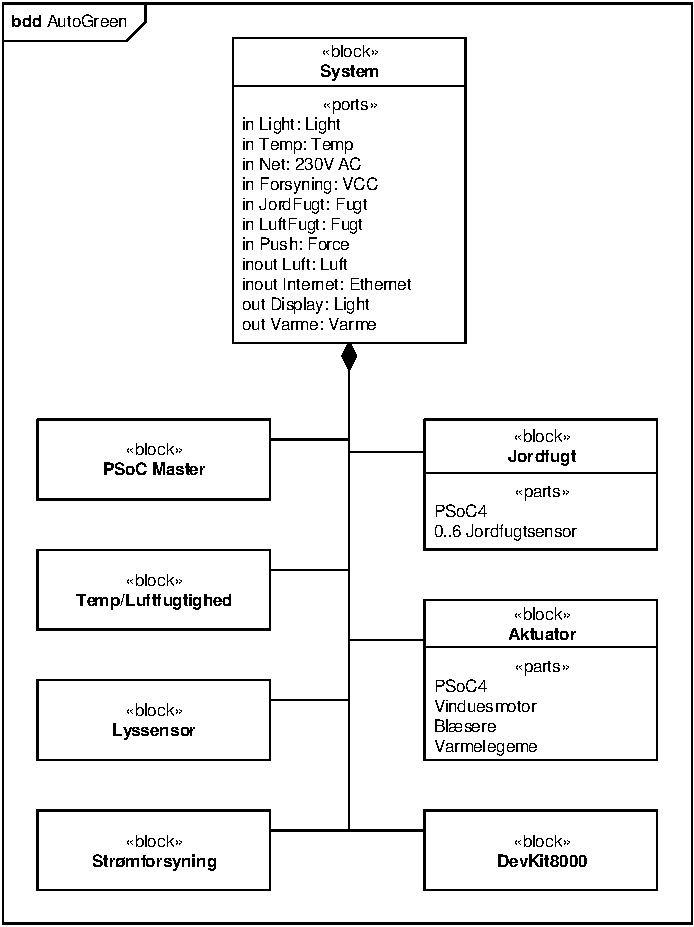
\includegraphics[width={\textwidth-2cm}, trim=0 0 0 0, clip=true] {../fig/bdd_system.pdf}
\caption{BDD for System.}
\label{fig:bdd_system}
\end{figure}

\clearpage

\subsection{IBD'er for System}

\begin{figure}[!h]
\centering 
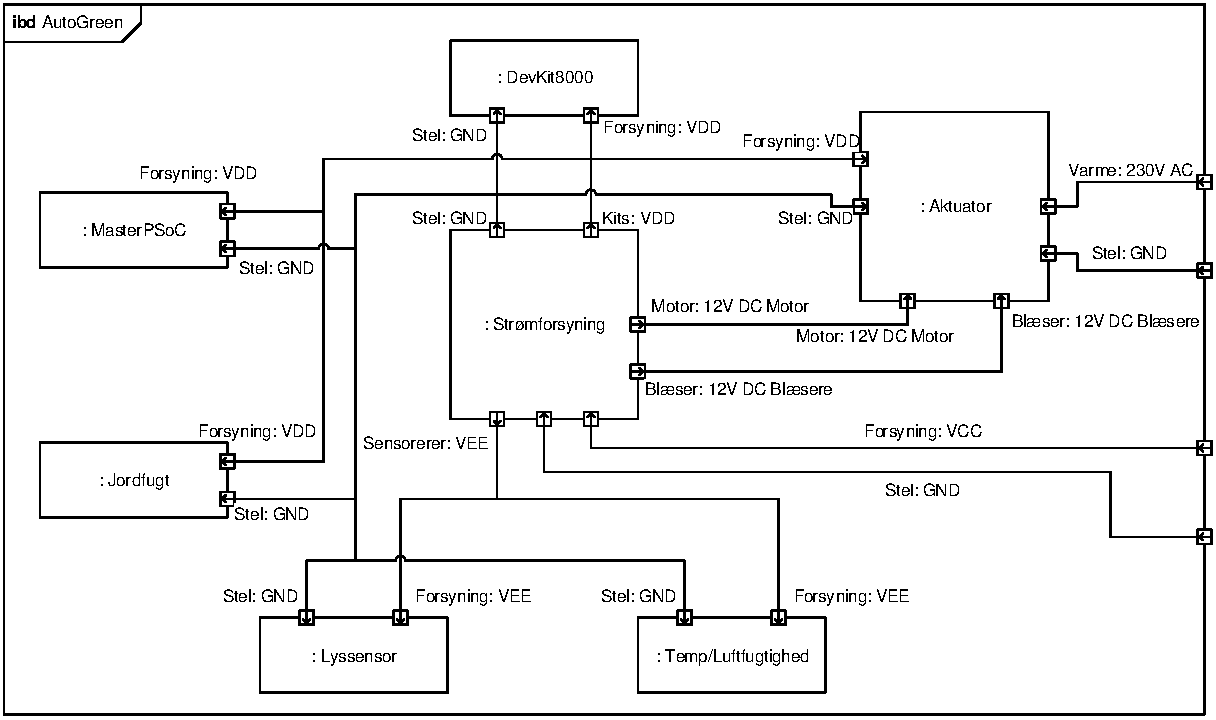
\includegraphics[width={\textheight-65 pt}, angle = 90] {../fig/ibd_system_forsyninger.pdf}
\caption{IBD for forsyninger i systemet.}
\label{fig:ibd_system_forsyn}
\end{figure}

\clearpage

\begin{figure}
\centering 
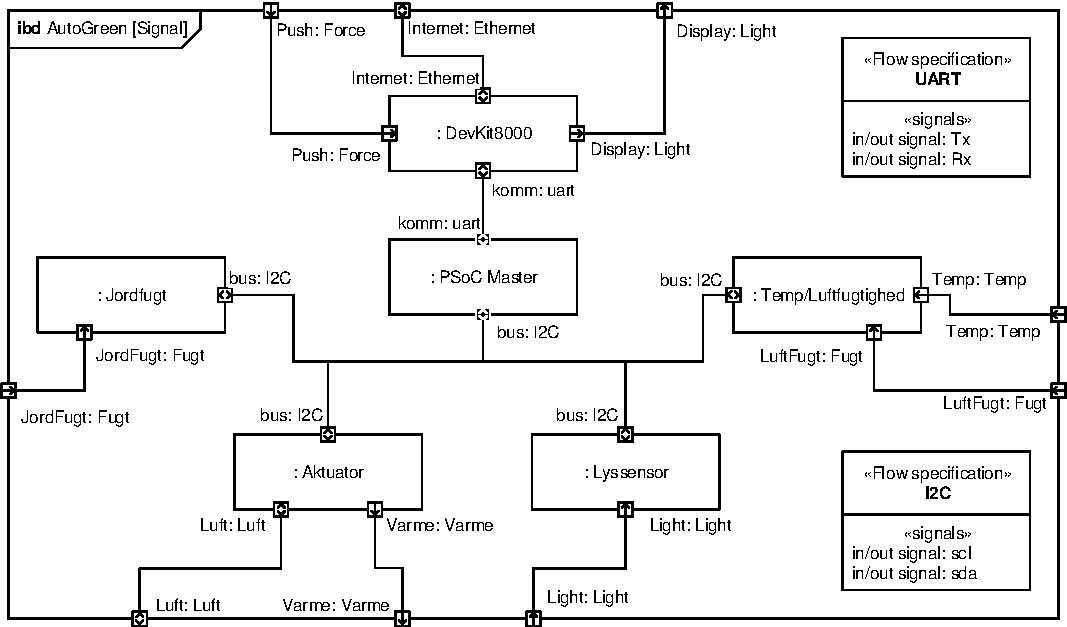
\includegraphics[width={\textheight-25 pt}, angle = 270] {../fig/ibd_system_signaler.pdf}
\caption{IBD for signaler i systemet.}
\label{fig:ibd_system_signal}
\end{figure}

\clearpage

\subsubsection{Strømforsyning}
Forsyner øvrig hardware i systemet, undtagen varmelegemet, Devkit8000 samt sensorer. Blokken forsynes fra en laboratorieforyning.
\subsubsection{DevKit8000}
Systemets brugerflade, er samtidigt controller for systemet. 
\subsubsection{PSoC Master}
PSoC4 Pioneer Kit, der har til opgave at kommunikere via UART med DevKit8000 og via \IIC med slaver.  
\subsubsection{Temp/Luftfugtighed}
Denne blok indeholder en sensor med \IIC interface og måler temperatur og luftfugtighed i det fysiske drivhus.
\subsubsection{Lyssensor}
Består af en sensor med \IIC interface og måler lysintensitet i det fysiske drivhus. 
\subsubsection{Jordfugt}
Denne blok indeholder op til seks analoge jordfugtsensorer, som vha. et PSoC4 Pioneer Kit er koblet på systemets \IIC bus.
\subsubsection{Aktuator}
Denne blok indeholder et PSoC4 Pioneer Kit, der fungerer som \IIC slave og styrer systemets aktuatorer. 

\clearpage

\subsection{IBD for Aktuator}

\begin{figure}[h]
\centering 
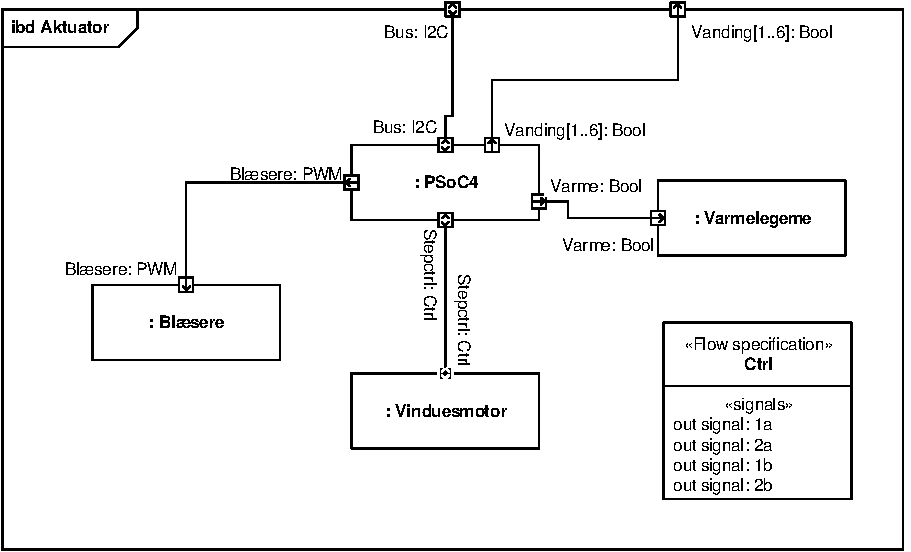
\includegraphics[width={\textwidth}, trim=0 0 0 0, clip=true] {../fig/ibd_aktuator.pdf}
\caption{IBD for Aktuator}
\label{fig:ibd_aktuator}
\end{figure}

\subsubsection{PSoC4}
PSoC blokken består af et PSoC4 Pioneer Kit, der agerer slave på \IIC bussen. 
\subsubsection{Vinduesmotor}
Denne blok består af en steppermotor, der styrer vinduet i det fysiske drivhus.
\subsubsection{Varmelegeme}
Varmelegeme med formål at hæve temperaturen i det fysiske drivhus. Varmelegemet styres af PSoC4 blokken, og det forsynes direkte fra elnettet (230V AC). 
\subsubsection{Blæsere}
Denne blok består af fire blæsere, som kan ventilere luften i det fysiske drivhus. Blæserne styres af PSoC4, og de forsynes fra Strømforsyning. 

\clearpage

\subsection{IBD for Jordfugt}

\begin{figure}[h]
\centering 
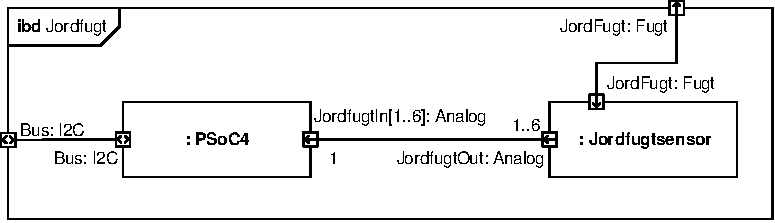
\includegraphics[width={\textwidth}] {../fig/ibd_jordfugt.pdf}
\caption{IBD for Jordfugt}
\label{fig:ibd_jordfugt}
\end{figure}

\subsubsection{PSoC4}
PSoC4 Pioneer Kit, der agerer slave på \IIC-bussen. 
\subsubsection{Jordfugtsensor}
Denne blok indeholder en analog sensor, der måler jordfugt ved en plante i det fysiske drivhus. Der kan kobles op til seks af disse til PSoC4.

\clearpage

\subsection{Signalbeskrivelser}
\label{subsec:signalbeskrivelser}

%\LTXtable{\textwidth}{Systemarkitektur/HWarkitektur/signalbeskrivelser.tex}

\begin{table}[h]
\begin{tabularx}{\textwidth}{| l | >{\raggedright}X | >{\raggedright}X | >{\raggedright\arraybackslash}X |>{\raggedright}X |}
\hline
	\textbf{Signaltype} & \textbf{Funktion} & \textbf{Tolerancer} & \textbf{Kommentar}\\ \hline
	VCC & Forsyning til strømforsyning & 12V $\pm$ 0,25V \newline 3A max. & Lab.forsyning  \\\hline	
	VDD & Forsyning til alle PSoC4 Pioneer Kits. & 5V DC $\pm$ 0.15V, \newline 0.5A max & - \\\hline
	VEE & Forsyning til sensorer & 3.3V DC $\pm$ 0.1V, \newline 0.1A max & - \\\hline
	12V DC Blæsere & Forsyning til blæsere. & 12V DC $\pm$ 0,25V, \newline 140mA max. & - \\\hline	
	12V DC Motor & Forsyning til vinduesmotor. & 12V $\pm$ 0,25V, \newline 500mA max. & - \\\hline
	230V AC & Forsyning til varmelegeme og DevKit8000. & 230V AC $\pm$ 10\%, \newline 50 Hz, \newline 0.3A max & - \\\hline
	Analog & Analogt målesignal fra jordfugtmåler. & 0-3.3V $\pm$ 0.1V & - \\\hline	
	Bool & Digitalt signal til styring af vanding og varmelegeme. & 0-3.3V & 1=True: 2.8-3.3V \newline 0=False: 0-0.4V \\\hline	
	Ctrl & Styring af stepper motor & 0-3.3V & 1=True: 2.8-3.3V \newline 0=False: 0-0.4V  \newline Består af fire signaler: \newline 1a, 2a, 1b, 2b \\\hline	
	GND & Stel & 0V & Reference \\\hline	
	I2C & Kommunikation mellem \IIC enheder. & 0-3.3V & 1=True: 2.8-3.3V \newline 0=False: 0-0.4V \newline Består af to signaler: \newline sca og scl \\\hline	
	UART & Kommunikation mellem DevKit8000 og Master & 0-5V & 1=True: 4.5-5V \newline 0=False: 0-0.4V \newline Består af 2 signaler: \newline Tx og Rx \\\hline	
	PWM & Styring af blæsere vha. pulsbreddemodulation. & 0-3.3V \newline 1 kHz & Duty cycle styres fra 0-100\% i trin fra 0-255. 0 svarer til 0\% og 255 svarer til 100\% \\\hline
\end{tabularx}
\caption{Beskrivelse af signaler.}
\label{tbl:signalbeskriv}
\end{table}

\clearpage

\section{Softwarearkitektur}

\subsection{Applikationsmodel}

Applikationsmodellen er valgt ud fra udviklernes synspunkt og bruges for at give overblik over hvilke klasser som skal laves, og hvilket ansvar de hver især har. Nedenstående UML skal ses som det overordnede system og menuklasserne er udeladt for at skabe overblik. 

\begin{figure}[!h]
\centering 
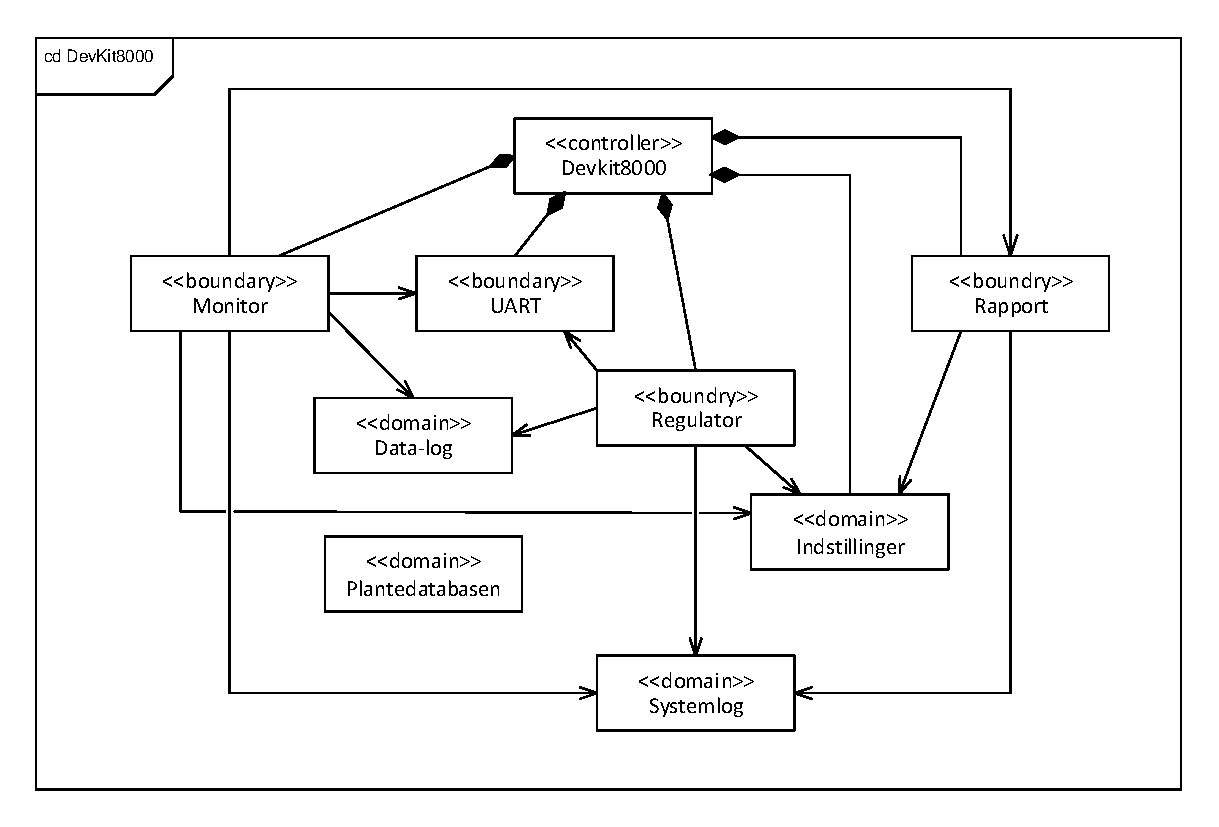
\includegraphics[scale=0.8] {../fig/UML_autogreen.pdf}
\caption{Application model for AutoGreen}
\label{fig:UML}
\end{figure}

\subsection{Controller-Klasser}

\subsubsection{DevKit8000}

DevKit8000 klassen skal initiere systemet og har derfter ansvaret for styring af processerne Regulering og Monitoring.
DevKit8000 klassen indeholder alle menuer beskrevet i menuoversigt. Brugeren kan interagere med klassen igennem menuerne.
Controller-klassen har igennem menuerne set i menuoversigten tilgang til de andre klasser i systemet.

\subsection{Boundary-Klasser}

\subsubsection{Monitor}

Monitorklassens primære opgave er at opsamle sensordata fra UART klassen og skrive dem til data-loggen. Der ud over skal Monitor skrive til System-log, hvis UART klassen rapporterer fejl ved dataoverførelse.

\subsubsection{Regulator}

Reguleringsklassen har ansvaret for at planterværdierne bliver overholdt. Den opnår dette ved at læse fra data-loggen, samt indstillinger som indeholder de virtuelle planter og hvis uregelmæssigheder findes blandt disse data, vil klassen tænde de fornødende akutuatorer gennem UART klassen. Der ud over skal Regulator skrive til System-log, hvis UART klassen rapporter fejl ved data overførelse.

\subsubsection{UART}

UARTklassen er grænsefladen mellem Devkittet og de sensorer/akutuatorer, der måtte eksistere i AutoGreen systemet.

\subsubsection{Rapport}

Rapportering indlæser E-mailkonfigurationer fra indstillinger, som bestemmer hvilken slags E-mails, der skal benyttes. Rapporting skal sende E-mail til brugeren dagligt, når der er kritisk klima i drivhuset, eller både dagligt og ved kritisk klima.

\subsection{Domain-Klasser}

\subsubsection{Data-log}

Data-loggen styrer en datastruktur. Det er dens opgave at modtage og indsætte målte data from drivhusklima i datastrukturen, samt hente informationer ud fra strukturen.

\subsubsection{System-log}

System-loggen har til ansvar at styre en datastruktur med henblik på at gemme de vigtigste systemhændelser og skal kunne tilgåes af brugeren senere.

\subsubsection{Indstillinger}

Indstillinger gemmer konfigurationer og indlæser dem i konfigurationsfilen, når regulering eller rapportering startes af brugeren. Den holder gemmer også de virtuelle planter og hvilken hardware der må bruges til at regulere temperaturen med. Der ud over bruges den også til at indstille og hente tiden i systemet.

\subsubsection{Plantedatabasen}

Plantedatabasen gemmer parametre for brugerdefinerede planter samt prækonfigurede planter og tilgås via en klasse menu.

\clearpage

\subsection{Menuoversigt}

Menuoversigten giver et overblik over de forskellige menuer og hvilke menuer, der giver tilgang til hinanden.

\begin{figure}[!h]
\centering 
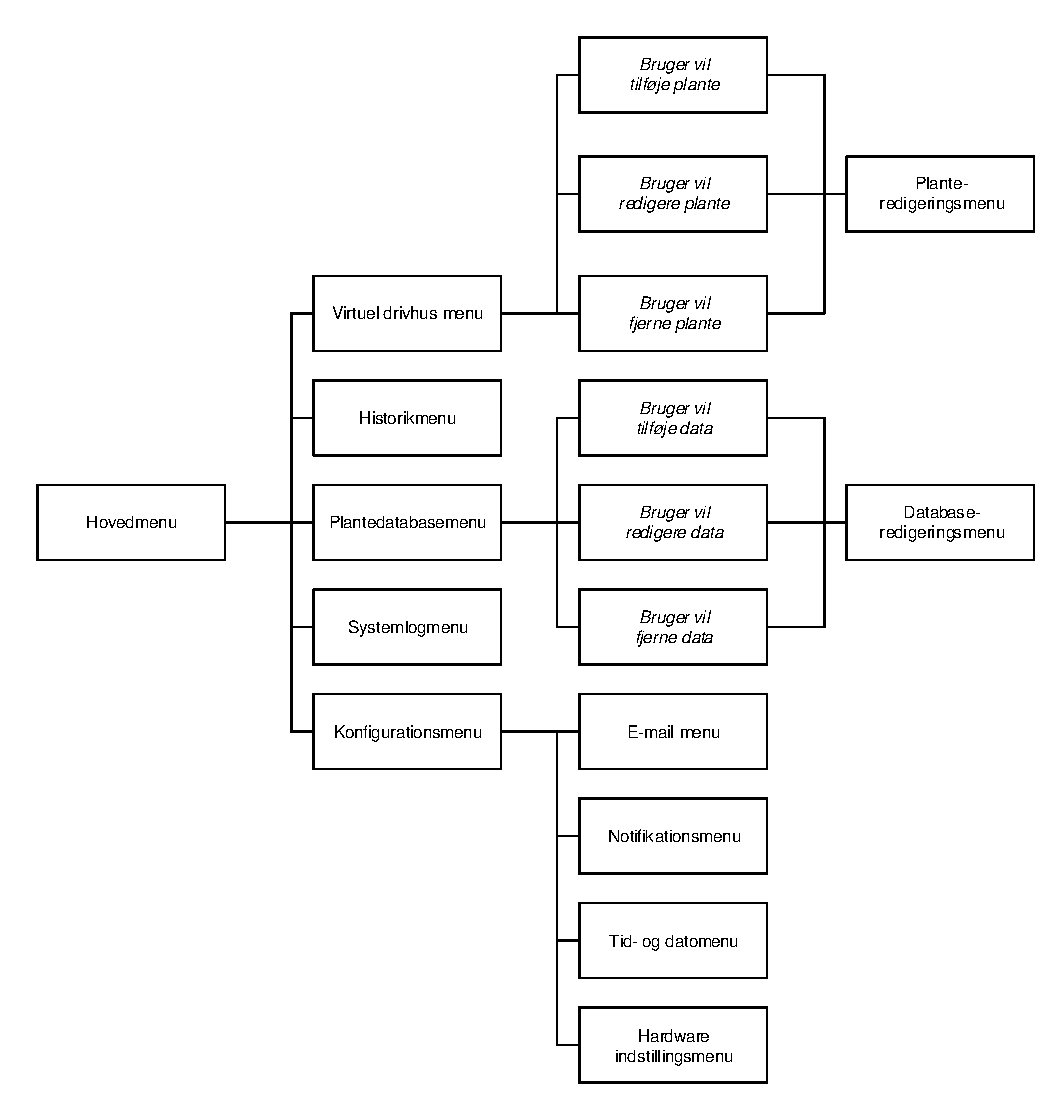
\includegraphics[scale=0.7] {../fig/menu_oversigt.pdf}
\caption{Oversigt over AutoGreen's menuer}
\label{fig:QTMenu}
\end{figure}

\subsection{Menubeskrivelse}
Menuoversigten er med til at give et overblik over hvordan de forskellige menuer tilgåes igennem systemet, og fra hvilke menuer man kan tilgå andre menuer. Hovedmenuen er som standard stedet, hvor brugeren starter, da er her muligt at monitorere drivhusklimaet. I hovedmenuen har brugeren mulighed for at tilgå de 5 undermenuer: virtuel drivhus-, historik-, plantedatabase-, systemlog- og konfigurationsmenu.

\subsubsection{Virtuelle drivhusmenu}
I det virtuelle drivhus har brugeren mulighed for at tilføje nye planter til drivhuset, redigere allerede tilstedeværende planter, og herunder slette planter fra drivhuset. Uanset ønsket skal brugeren tilgå planteredigeringsmenuen.

\subsubsection{Historikmenu}
I historikmenuen har brugeren mulighed for at se data over drivhuset op til et år tilbage.

\subsubsection{Plantedatabasemenu}
I plantedatabasemenuen har brugeren mulighed for at tilføje nye planter til databasen. Ved tryk på 'tilføj plante' oprettes en ny tom virtuel plante i databasen. Denne virtuelle plante åbnes i databaseredigeringsmenuen, hvor dens paramentre kan indstilles efter behov. Hvis brugeren ønsker at redigere allerede oprettede planter eller slette disse, kan brugeren trykke på den ønskede plante. Den valgte plante vil blive åbnet gennem databaseredigeringsmenuen, og det er her muligt at redigere eller slette planten.

\subsubsection{Systemlogmenu}
I systemloggen har brugeren mulighed for at se systemhændelser, f.eks. hvis systemet vælger at åbne et vindue, starte en blæser, eller bruge varmelegemet.

\subsubsection{Konfigurationsmenu}
I konfigurationsmenu har brugeren mulighed for at tilgå 4 undermenuer: E-mailmenu, Notifikationsmenu, Tid- og datomenu, samt Hardware Indstillingsmenu.

\subsubsection{E-mailmenu} \label{sec:mailmenu}
I E-mailmenuen, vises 3 kolonner, hvor brugeren har mulighed for at indtaste E-mail adresse, som skal modtage notifiktationer. 

\subsubsection{Notifikationsmenu} 
I notifikationsmenuen har brugeren mulighed for at slå notifikationer til og fra for både advarsels-notifikationer og daglige notifikationer. 

\subsubsection{Tids- og datomenu} 
I Tids- og datomenuen har brugeren mulighed for at ændre dato og tid. 

\subsubsection{Hardware Indstillingsmenu} 
I Hardware Indstillingsmenu har brugeren mulighed for at vælge hvilke akutuatorer drivhuset skal bruge. Hvis brugeren ønsker at spare strøm, kan blæser og varmelegeme fravælges til regulering temperaturen.

\clearpage

\clearpage
\section{Protokol for UART} \label{UART_Protokol} %TODO Skift dette label ud med 'sec:UART_protokol' her og i samtlige steder den bliver brugt :)

I projektforløbets senere faser deles arbejdet op mellem en HW- og en SW-gruppe. SW gruppen har ansvar for design og implementering af SW på DevKit8000, mens HW gruppen har ansvar for design og realisering af HW og SW på PSoC4 Pioneer Kits. UART kommunikationen mellem PSoC Master og DevKit8000 defineres derved som grænsefladen mellem HW og SW, omend en del af funktionaliteten på PSoC4 Pioneer Kits realiseres vha. SW.

\subsection{UART indstillinger}

\begin{itemize}
\item Baud rate: 9600 
\item Antal bits: 8
\item Antal stop bits: 1
\item Paritet: Even
\end{itemize}

\subsection{Datavalidering}

For at sikre validering af data sendt fra DevKit8000 til PSoC4 Master, sendes der altid svar tilbage fra PSoC4 Master til DevKit8000. Svaret består af en gentagelse af den modtagne kommando og evt. nogle dataværdier. \newline
Såfremt der går noget galt i I2C kommunikationen i HW delen af systemet, sendes en fejlkode til DevKit8000. 
Derved er der mulighed for at SW på DevKit8000 kan logge fejlhændelser i systemloggen, og fx gensende kommandoer eller kassere data. \newline
Da hver enkelt byte, der sendes via UART er vedlagt en paritetsbit sikrer vi os til dels at hver byte overføres korrekt. \newline
Når DevKit8000 sender en kommando via UART skal PSoC Master svare indenfor 2 sekunder. Såfremt dette ikke sker, sendes kommandoen igen mindst to gange. Alle kommandoer udføres serielt, hvilket vil sige at næste kommando ikke sendes før der er modtaget svar på den foregående.

\subsection{Kommandoer}

\LTXtable{\textwidth}{Systemarkitektur/UARTprotokol/kommandoer}



\chapter{Hardware Design} \label{ch:HwDesign}

\section{Version}
\begin{table}[h]
	\centering
	\begin{tabularx}{\textwidth - 2cm}{|l|l|l|X|}
	\hline
	Dato	& Version	& Initialer & Ændring	\\ \hline
	30. marts & 1 & MHG & I2C Protokol og design af Aktuator. \\ \hline
	8. april & 2 & MHG & Mindre rettelser i Aktuatordesign. \\ \hline
	10. april & 3 & MHG & Skrevet det sidste (varmelegeme) design i aktuator blokken. \\\hline 
	23. april & 4 & MHG & Lavet mindre rettelser i et par diagrammer. \\\hline
	27. april & 5 & MHG & Skrevet design for Strømforsyning. \\\hline
	1. maj & 6 & MHG & Skrevet design for Slave Jordfugt. \\\hline
	\end{tabularx}
\end{table}

\section{\IIC Protokol} \label{sec:I2C_protokol}
Dette afsnit omhandler kommunikationen mellem alle \IIC kommunikerende komponenter i projektet.

\subsection{Temp-/Luftfugtighedssensor}
Information om Temperatur- og Luftfugtighedssensor er fundet under komponentens datasheet. Bilag 004 \cite{lib:TempHum_I2C}.

%Slave Temp-/Luftfugtihed
\begin{table}[h]
\centering
\begin{tabularx}{0.6\textwidth}{| X | X |} 			\hline
\textbf{Slave:} 		& Temp-/Luftfugtighed		\\ \hline
\textbf{Adresse:}		& 0x27						\\ \hline
\textbf{Bemærkninger:}	& scl: 100-400 kHz			\\ \hline
\end{tabularx}
\caption{\IIC Oplysninger for Temp-/Luftfugtigedhedssensor}
\label{tbl:I2CTempLuftOplysninger}
\end{table}


Når der skal læses data fra sensoren, sker det jf. Figur \ref{fig:I2CTempLuftProtokol}, fundet under Bilag 004 side 2 \cite{lib:TempHum_I2C}.


\begin{figure}[h]
\centering
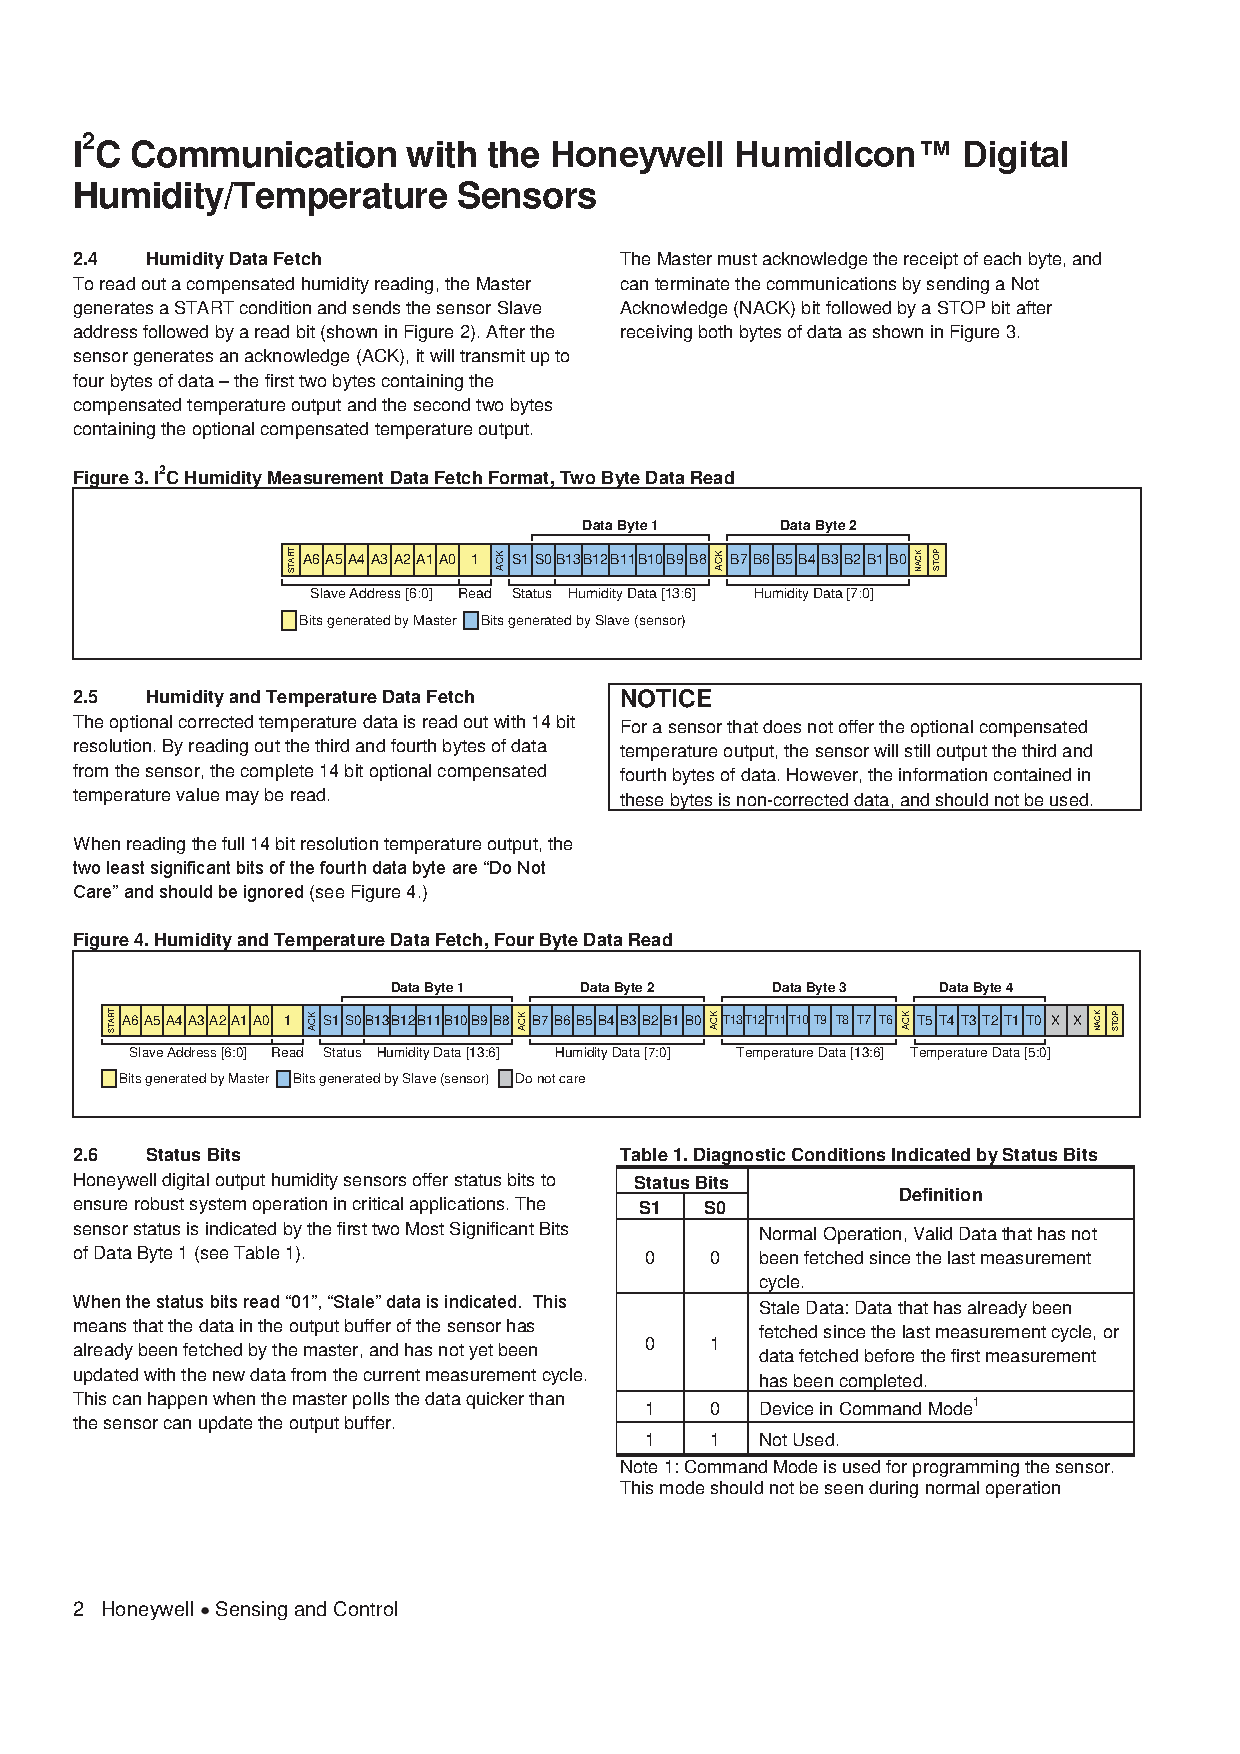
\includegraphics[width=\textwidth - 1 cm, clip=true, trim=48 319 55 471]{../fig/I2CTempLuftProtokol.pdf}
\caption{\IIC protokol for Temp-/Luftfugtighedssensor}
\label{fig:I2CTempLuftProtokol}
\end{figure}

\clearpage

\subsection{Slave Aktuator}
%Slave Aktuator
\begin{table}[h]
\centering
\begin{tabularx}{0.6\textwidth}{| X | X |} 			\hline
\multicolumn{2}{ | l | }{\textbf{Adresse:} 0x42} 	\\ \hline
\textbf{Kommando} 		& \textbf{Beskrivelse}		\\ \hline
WriteAdjustWindow		& Åbning/Lukning af vindue	\\ \hline
WriteAdjustHeat			& Tænd/Sluk for varme		\\ \hline
WriteAdjustVentilation	& Juster ventilation		\\ \hline
WriteAdjustIrrigation	& Juster vanding			\\ \hline
ReadStatus				& Anmodning om status		\\ \hline
\end{tabularx}
\caption{\IIC Kommandoer for Slave Aktuator}
\label{tbl:I2CAktuatorKommandoer}
\end{table}



%WriteAdjustWindow
\begin{table}[h]
\centering
\begin{tabularx}{0.6\textwidth}{| >{\centering\arraybackslash}X | >{\centering\arraybackslash}X | >{\centering\arraybackslash}X | >{\centering\arraybackslash}X | >{\centering\arraybackslash}X | >{\centering\arraybackslash}X | >{\centering\arraybackslash}X | >{\centering\arraybackslash}X |}	\hline
W7 & W6 & W5 & W4 & W3 & W2 & W1 & W0				\\ \hline
\multicolumn{2}{ | l | }{0x0} 						&
\multicolumn{2}{  l | }{Don't Cares}				&
\multicolumn{4}{  l | }{Position for vindue,}
\\
\multicolumn{2}{ | l | }{} 							&
\multicolumn{2}{  l | }{}							&
\multicolumn{4}{  l | }{0x0 = lukket, 0xF = åben}
\\ \hline
\end{tabularx}
\caption{\IIC Kommando WriteAdjustWindow}
\label{tbl:I2CAktuatorKommandoWriteAdjustWindow}
\end{table}



%WriteAdjustHeat
\begin{table}[h]
\centering
\begin{tabularx}{0.6\textwidth}{| >{\centering\arraybackslash}X | >{\centering\arraybackslash}X | >{\centering\arraybackslash}X | >{\centering\arraybackslash}X | >{\centering\arraybackslash}X | >{\centering\arraybackslash}X | >{\centering\arraybackslash}X | >{\centering\arraybackslash}X |}	\hline
H7 & H6 & H5 & H4 & H3 & H2 & H1 & H0				\\ \hline
\multicolumn{2}{ | l | }{0x1} 						&
\multicolumn{3}{  l | }{Don't Care}					&
\multicolumn{3}{  l | }{Tænd/Sluk}
\\
\multicolumn{2}{ | l | }{} 							&
\multicolumn{3}{  l | }{}							&
\multicolumn{3}{  l | }{varmelegeme,}
\\
\multicolumn{2}{ | l | }{} 							&
\multicolumn{3}{  l | }{}							&
\multicolumn{3}{  l | }{0x0 = off, 0x7 = on}
\\ \hline
\end{tabularx}
\caption{\IIC Kommando WriteAdjustHeat}
\label{tbl:I2CAktuatorKommandoWriteAdjustHeat}
\end{table}

\clearpage

%WriteAdjustVentilation
\begin{table}[h]
\centering
\begin{tabularx}{0.6\textwidth}{| >{\centering\arraybackslash}X | >{\centering\arraybackslash}X | >{\centering\arraybackslash}X | >{\centering\arraybackslash}X | >{\centering\arraybackslash}X | >{\centering\arraybackslash}X | >{\centering\arraybackslash}X | >{\centering\arraybackslash}X |}	\hline
V7 & V6 & V5 & V4 & V3 & V2 & V1 & V0				\\ \hline
\multicolumn{2}{ | l | }{0x2} 						&
\multicolumn{3}{  l | }{Don't Care}					&
\multicolumn{3}{  l | }{Tænd/Sluk}
\\
\multicolumn{2}{ | l | }{} 							&
\multicolumn{3}{  l | }{}							&
\multicolumn{3}{  l | }{ventilation,}
\\
\multicolumn{2}{ | l | }{} 							&
\multicolumn{3}{  l | }{}							&
\multicolumn{3}{  l | }{0x0 = off, 0x7 = on}
\\ \hline
\end{tabularx}
\caption{\IIC Kommando WriteAdjustVentilation}
\label{tbl:I2CAktuatorKommandoWriteAdjustVentilation}
\end{table}



%WriteAdjustIrrigation
\begin{table}[h]
\centering
\begin{tabularx}{0.6\textwidth}{| >{\centering\arraybackslash}X | >{\centering\arraybackslash}X | >{\centering\arraybackslash}X | >{\centering\arraybackslash}X | >{\centering\arraybackslash}X | >{\centering\arraybackslash}X | >{\centering\arraybackslash}X | >{\centering\arraybackslash}X |}	\hline
I7 & I6 & I5 & I4 & I3 & I2 & I1 & I0				\\ \hline
\multicolumn{2}{ | l | }{0x3} 						&
\multicolumn{6}{  l | }{Værdi for pins til vanding,}
\\
\multicolumn{2}{ | l | }{} 							&
\multicolumn{6}{  l | }{I5: nr. 6 – I0: nr. 1,}
\\
\multicolumn{2}{ | l | }{} 							&
\multicolumn{6}{  l | }{1 = on, 0 = off}
\\ \hline
\end{tabularx}
\caption{\IIC Kommando WriteAdjustIrrigation}
\label{tbl:I2CAktuatorKommandoWriteAdjustIrrigation}
\end{table}



%ReadStatus
\begin{table}[!h]
\begin{tabularx}{\textwidth}{| >{\centering\arraybackslash}X | >{\centering\arraybackslash}X | >{\centering\arraybackslash}X | >{\centering\arraybackslash}X | >{\centering\arraybackslash}X | >{\centering\arraybackslash}X | >{\centering\arraybackslash}X | >{\centering\arraybackslash}X | >{\centering\arraybackslash}X | >{\centering\arraybackslash}X | >{\centering\arraybackslash}X | >{\centering\arraybackslash}X | >{\centering\arraybackslash}X | >{\centering\arraybackslash}X | >{\centering\arraybackslash}X | >{\centering\arraybackslash}X |}	\hline
W3 & W2 & W1 & W0 & H2 & H1 & H0 & V2 & V1 & V0 & I5 & I4 & I3 & I2 & I1 & I0				\\ \hline
\multicolumn{4}{ | l | }{Position for vindue,} 			&
\multicolumn{3}{  l | }{Status for}						&
\multicolumn{3}{  l | }{Status for}						&
\multicolumn{6}{  l | }{Status for pins til vanding,}
\\
\multicolumn{4}{ | l | }{0x0 = lukket,} 				&
\multicolumn{3}{  l | }{Varmelegeme,}					&
\multicolumn{3}{  l | }{ventilation,}					&
\multicolumn{6}{  l | }{I5: nr. 6 – I0: nr. 1,}	
\\
\multicolumn{4}{ | l | }{0xF = åben} 					&
\multicolumn{3}{  l | }{1 = on,}						&
\multicolumn{3}{  l | }{0x0 = off,}						&
\multicolumn{6}{  l | }{1 = on,}
\\
\multicolumn{4}{ | l | }{} 								&
\multicolumn{3}{  l | }{0 = off}						&
\multicolumn{3}{  l | }{0x7 = on}						&
\multicolumn{6}{  l | }{0 = off}					
\\ \hline
\end{tabularx}
\caption{\IIC Kommando ReadStatus}
\label{tbl:I2CAktuatorKommandoReadStatus}
\end{table}

\clearpage
\section{PSoC Master} \label{sec:PSoC_Master_design}

På Figur \ref{fig:Master_PSoC_klassediagram} ses klassediagrammet for Master PSoC. Der er blevet designet 4 klasser der håndterer hver sin del af arbejdet, som masteren skal udføre. Der er valgt to boundaryklasser, som håndterer kommunikation over hhv. UART og \IIC. Udover dette er der en domæneklasse, som indeholder alle de målte dataværdier, der er modtaget af sensorerne. 

\begin{figure}[h]
\centering 
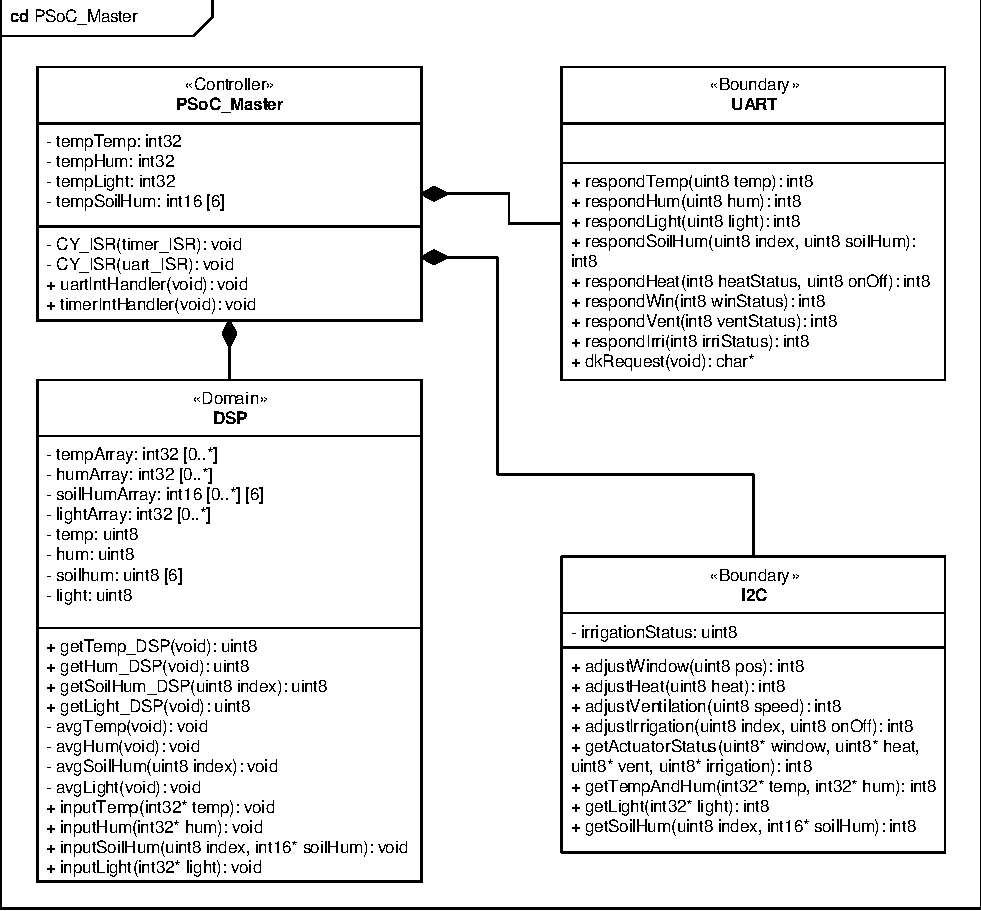
\includegraphics[width={\textwidth}, trim=0 0 0 0, clip=true] {../fig/cd_PSoC_master.pdf}
\caption{Klassediagram for Master PSoC}
\label{fig:Master_PSoC_klassediagram}
\end{figure}

\clearpage

\subsection{Klassebeskrivelser}

%++++++++++++ Controller PSoC Master klassen ++++++++++++++
\subsubsection{Controllerklasse PSoC\_Master}

\textbf{Attributter}

\begin{table}[h]
\begin{tabularx}{\textwidth}{| >{\raggedright\arraybackslash}X | >{\raggedright\arraybackslash}X | >{\raggedright\arraybackslash}p{10 cm} |} \hline
\texttt{tempTemp} & \texttt{int32} & Midlertidig variabel til opbevaring af temperatur. \\\hline
\texttt{tempHum} & \texttt{int32} & Midlertidig variabel til opbevaring af luftfugtighed. \\\hline
\texttt{tempLight} & \texttt{int32} & Midlertidig variabel til opbevaring af lysintensitet. \\\hline
\texttt{tempSoilHum} & \texttt{int16} & Midlertidig variabel til opbevaring af jordfugtighed. \\\hline
\end{tabularx}
\caption{Attributter for klassen PSoC\_Master}
\label{table:PSoC_Master_attributter}
\end{table}

\textbf{Metoder}

%========================= CY_ISR(timer_ISR) ==============

\begin{table}[h]
\begin{tabularx}{\textwidth}{| >{\raggedright\arraybackslash}p{2.5 cm} | >{\raggedright\arraybackslash}X |} \hline
Prototype & \texttt{void CY\_ISR(timer\_ISR)} \\\hline
Parametre & \texttt{timer\_ISR} \newline Vector for den givne interrupt servicerutine. \\\hline
Returværdi & - \\\hline
Beskrivelse & Denne interrupt service rutine bliver kaldt, når en ønsket tidsperiode er forløbet. Rutinen kalder metoder i boundaryklassen \IIC, der varetager indhentning af data fra sensorer.  \\\hline
\end{tabularx}
\caption{CY\_ISR(timer\_ISR)}
\label{table:CY_ISR(timer_ISR)}
\end{table}

%========================= CY_ISR(uart_ISR) ==============

\begin{table}[h]
\begin{tabularx}{\textwidth}{| >{\raggedright\arraybackslash}p{2.5 cm} | >{\raggedright\arraybackslash}X |} \hline
Prototype & \texttt{void CY\_ISR(uart\_ISR)} \\\hline
Parametre & \texttt{uart\_ISR} \newline 
Vector for den givne interrupt servicerutine. \\\hline
Returværdi & - \\\hline
Beskrivelse & Denne interrupt service rutine bliver kaldt, når der modtages noget på UART fra DevKit8000. Rutinen kalder metoder i boundaryklasserne \IIC og UART. Formålet med interrupten er at håndtere forskellige typer af forespørgsler. \\\hline
\end{tabularx}
\caption{CY\_ISR(uart\_ISR)}
\label{table:CY_ISR(uart_ISR)}
\end{table}

%========================= FLERE UART FUNKTIONER ==============

\newpage

\subsubsection{Boundaryklasse UART}
%+++++++++++++++++++++++++ Boundary UART ++++++++++++++++++++
\textbf{Metoder}

%========================= respondTemp ==============

\begin{table}[h]
\begin{tabularx}{\textwidth}{| >{\raggedright\arraybackslash}p{2.5 cm} | >{\raggedright\arraybackslash}X |} \hline
Prototype & \texttt{int8 respondTemp(uint8 temp)} \\\hline
Parametre & \texttt{uint8 temp} \newline
Den nyeste midlede temperatur hentet fra domæneklassen DSP. 
 \\\hline
Returværdi & \texttt{int8} \newline
Er denne værdi nul er der blevet returneret en gyldig værdi. Hvis værdien er -1 er der blevet returneret ’XT’ over UART. \\\hline
Beskrivelse & Hvis parameter værdien ligger inden for decimalværdien 1-200 (begge inklusive), skal metoden sende en char ’T’, efterfulgt af temp parameteren, over UART. Er værdien er lig nul, skal metoden sende strengen ”XT".   \\\hline
\end{tabularx}
\caption{respondTemp}
\label{table:respondTemp}
\end{table}

%========================= respondHum ==============

\begin{table}[h]
\begin{tabularx}{\textwidth}{| >{\raggedright\arraybackslash}p{2.5 cm} | >{\raggedright\arraybackslash}X |} \hline
Prototype & \texttt{ int8 respondHum(uint8 hum)} \\\hline
Parametre & \texttt{uint8 hum} \newline
Den nyeste midlede luftfugtighed hentet fra domæneklassen DSP. 
 \\\hline
Returværdi & \texttt{int8} \newline
Er denne værdi nul er der blevet returneret en gyldig værdi. Hvis værdien er -1 er der blevet returneret ’XA’ over UART. \\\hline
Beskrivelse & Hvis parameter værdien ligger inden for decimalværdien 1-100 (begge inklusive), skal metoden sende en char ’A’, efterfulgt af hum parameteren, over UART. Hvis værdien er lig nul, skal metoden sende strengen ”XA".    \\\hline
\end{tabularx}
\caption{respondHum}
\label{table:respondHum}
\end{table}

%========================= respondLight ==============

\begin{table}[h]
\begin{tabularx}{\textwidth}{| >{\raggedright\arraybackslash}p{2.5 cm} | >{\raggedright\arraybackslash}X |} \hline
Prototype & \texttt{int8 respondLight(uint8 light)} \\\hline
Parametre & \texttt{uint8 light} \newline
Den nyeste midlede lysintensitet hentet fra domæneklassen DSP. 
 \\\hline
Returværdi & \texttt{int8} \newline
Er denne værdi nul er der blevet returneret en gyldig værdi. Hvis værdien er -1 er der blevet returneret ’XL’ over UART.\\\hline
Beskrivelse & Hvis parameter værdien ligger inden for decimalværdien 1-100 (begge inklusive), skal metoden sende en char ’L’ efterfulgt af light parameteren over UART. Hvis værdien er lig nul, skal metoden sende strengen ”XL".     \\\hline
\end{tabularx}
\caption{respondLight}
\label{table:respondLight}
\end{table}

%========================= respondSoilHum ==============

\begin{table}[h]
\begin{tabularx}{\textwidth}{| >{\raggedright\arraybackslash}p{2.5 cm} | >{\raggedright\arraybackslash}X |} \hline
Prototype & \texttt{int8 respondSoilHum(uint8 index, uint8 soilHum)} \\\hline
Parametre & \texttt{uint8 soilHum} \newline
Den nyeste midlede jordfugtighed hentet fra domæneklassen DSP. \newline
\texttt{uint8 index} \newline
Indexet fortæller hvilket sensornummer der svares fra. \\\hline
Returværdi & \texttt{int8} \newline
Er denne værdi nul er der blevet returneret en gyldig værdi. Hvis værdien er -1 er der blevet returneret ’XS’ over UART.\\\hline
Beskrivelse & Hvis parameter værdien ligger inden for decimalværdien 1-10 (begge inklusive), skal metoden sende en char ’S’, efterfulgt af index og soilHum parametrene over UART. Hvis værdien for soilHum er lig nul, skal metoden sende strengen ”XS". \\\hline
\end{tabularx}
\caption{respondSoilHum}
\label{table:respondSoilHum}
\end{table}

%========================= respondHeat ==============

\begin{table}[h]
\begin{tabularx}{\textwidth}{| >{\raggedright\arraybackslash}p{2.5 cm} | >{\raggedright\arraybackslash}X |} \hline
Prototype & \texttt{int8 respondHeat(uint8 heatStatus, uint8 On)} \\\hline
Parametre & \texttt{uint8 heatStatus} \newline
Returværdien fra funktionen adjustHeat i boundaryklassen \IIC; fortæller om kommunikationen over \IIC er gået godt. \newline
\texttt{uint8 On} \newline
Returværdi til UART afhængig af hvilken kommando, der blev kaldt. 0 = off, 0 != on.
 \\\hline
Returværdi & \texttt{int8} \newline
Er denne værdi nul er kommunikationen over \IIC gennemført. Hvis værdien er
-1 er der blevet returneret en værdi tilsvarene requesten fra DevKit8000 over UART (se UART protokol side \pageref{UART_Protokol}) og der er sket en fejl i kommunikationen over \IIC.
\\\hline
Beskrivelse & Hvis parameter værdien er lig nul, sendes en char tilsvarene requesten over UART. Hvis værdien er lig -1, sendes sendes en tilsvarene fejlmeddelelse. \\\hline
\end{tabularx}
\caption{respondHeat}
\label{table:respondHeat}
\end{table}

%========================= respondWin ==============

\begin{table}[h]
\begin{tabularx}{\textwidth}{| >{\raggedright\arraybackslash}p{2.5 cm} | >{\raggedright\arraybackslash}X |} \hline
Prototype & \texttt{int8 respondWin(int8 winStatus)} \\\hline
Parametre & \texttt{int8 winStatus} \newline
Returværdien fra funktionen adjustWin i boundaryklassen \IIC. Fortæller om kommunikationen via. \IIC til vinduesaktuatoren er forløbet godt.  
 \\\hline
Returværdi & \texttt{int8} \newline
Er denne værdi nul er kommunikationen over \IIC gennemført. Hvis værdien er -1 er der blevet returneret ’XK’ over UART og der er sket en fejl i kommunikationen over \IIC.\\\hline
Beskrivelse & Hvis parameter værdien er lig nul, sendes en char ’K’ over UART. Hvis værdien er lig -1, sendes strengen ”XK". \\\hline
\end{tabularx}
\caption{respondWin}
\label{table:respondWin}
\end{table}

%========================= respondVent ==============

\begin{table}[h]
\begin{tabularx}{\textwidth}{| >{\raggedright\arraybackslash}p{2.5 cm} | >{\raggedright\arraybackslash}X |} \hline
Prototype & \texttt{int8 respondVent(int8 ventStatus)} \\\hline
Parametre & \texttt{int8 ventStatus} \newline
Returværdien fra funktionen adjustVent i boundaryklassen \IIC. Fortæller om kommunikationen via \IIC til ventilatoraktuatoren er forløbet uden problemer.   
 \\\hline
Returværdi & \texttt{int8} \newline
Er denne værdi 0, er kommunikationen over \IIC gennemført. Hvis værdien er 
-1 er der blevet returneret ’XV’ over UART og der er sket en fejl i kommunikationen over \IIC.
\\\hline
Beskrivelse & Hvis parameterværdien er lig nul, sendes en char ’V’ over UART, hvilket indikerer at det er gået godt. Hvis værdien er lig -1, sendes strengen ”XV". \\\hline
\end{tabularx}
\caption{respondVent}
\label{table:respondVent}
\end{table}

%========================= respondIrri ==============

\begin{table}[h]
\begin{tabularx}{\textwidth}{| >{\raggedright\arraybackslash}p{2.5 cm} | >{\raggedright\arraybackslash}X |} \hline
Prototype & \texttt{int8 respondIrri(int8 irriStatus)} \\\hline
Parametre & \texttt{int8 irriStatus} \newline
Returværdien fra funktionen adjustIrrigation i boundaryklassen \IIC. Fortæller om kommunikationen via \IIC til irrigationsaktuatoren er forløbet uden problemer.   
 \\\hline
Returværdi & \texttt{int8} \newline
Er denne værdi nul, er kommunikationen over \IIC gennemført. Hvis værdien er 
-1 er der blevet returneret ’XF’ over UART og der er sket en fejl i kommunikationen over \IIC.
\\\hline
Beskrivelse & Hvis parameterværdien er lig nul, sendes en char ’F’ over UART, hvilket indikerer at det er gået godt. Hvis værdien er lig 
-1, sendes strengen ”XF". \\\hline
\end{tabularx}
\caption{respondIrri}
\label{table:respondIrri}
\end{table}

\clearpage

%+++++++++++++++++++++++++ I2C klassen ++++++++++++++
\subsubsection{Boundaryklasse \IIC}

\textbf{Attributter}

\begin{table}[h]
\begin{tabularx}{\textwidth}{| >{\raggedright\arraybackslash}X | >{\raggedright\arraybackslash}X | >{\raggedright\arraybackslash}p{8 cm} |} \hline
Navn & Type & Beskrivelse \\\hline
\texttt{irrigationStatus} & \texttt{uint8} & Indeholder den aktuelle status for vandingsaktuatorer (tændt eller slukkede). Bit 0 – 5 er hhv. aktuatorerne fra 1 – 6. Nul betyder slukket og et betyder tændt. \\\hline
\end{tabularx}
\caption{Attributter for klassen \IIC}
\label{table:IIC_attributter}
\end{table}

\textbf{Metoder}

%========================= adjustWindow ==============

\begin{table}[h]
\begin{tabularx}{\textwidth}{| >{\raggedright\arraybackslash}p{2.5 cm} | >{\raggedright\arraybackslash}X |} \hline
Prototype & \texttt{int8 adjustWindow(uint8 pos)} \\\hline
Parametre & \texttt{uint8 pos} \newline 
Den ønskede status for vinduet. Kan være hhv. 0xFF for åben og 0x00 for lukket. \\\hline
Returværdi & \texttt{int8} \newline
Er værdien 0, er kommunikation via \IIC gået godt. Hvis værdien er -1, er der sket en fejl. \\\hline
Beskrivelse & Metoden kan justere positionen for vinduet i drivhuset. Sender kommandoen ”WriteAdjustWindow” via \IIC bussen (se \IIC protokol på side \pageref{sec:I2C_protokol}). \\\hline
\end{tabularx}
\caption{adjustWindow}
\label{table:adjustWindow}
\end{table}

%========================= adjustHeat ==============

\begin{table}[h]
\begin{tabularx}{\textwidth}{| >{\raggedright\arraybackslash}p{2.5 cm} | >{\raggedright\arraybackslash}X |} \hline
Prototype & \texttt{int8 adjustHeat(uint8 heat)} \\\hline
Parametre & \texttt{uint8 heat} \newline 
Bestemmer intensiteten af varmen, 0x00 er ingen varme, 0xFF er fuld varme. \\\hline
Returværdi & \texttt{int8} \newline
Er værdien 0, er kommunikation via \IIC gået godt. Hvis værdien er -1, er der sket en fejl (se \IIC protokol på side \pageref{sec:I2C_protokol}). \\\hline
Beskrivelse & Slukker eller tænder for varmeaktuatoren. Sender kommandoen ”WriteAdjustHeat” via \IIC bussen (se \IIC protokol på side \pageref{sec:I2C_protokol}). \\\hline
\end{tabularx}
\caption{adjustHeat}
\label{table:adjustHeat}
\end{table}

%========================= adjustVentilation ==============

\begin{table}[h]
\begin{tabularx}{\textwidth}{| >{\raggedright\arraybackslash}p{2.5 cm} | >{\raggedright\arraybackslash}X |} \hline
Prototype & \texttt{int8 adjustVentilation(uint8 speed)} \\\hline
Parametre & \texttt{uint8 speed} \newline 
Beskriver ventilatoraktuatornes tilstand. 0x00 svarer til slukket og 0xFF svarer til fuld hastighed. \\\hline
Returværdi & \texttt{int8} \newline
Er værdien 0, er kommunikation via \IIC gået godt. Hvis værdien er -1, er der sket en fejl (se \IIC protokol på side \pageref{sec:I2C_protokol}). \\\hline
Beskrivelse & Slukker eller tænder for ventilation. Sender kommandoen ”WriteAdjustVentilation” via \IIC bussen (se \IIC protokol på side \pageref{sec:I2C_protokol}). \\\hline
\end{tabularx}
\caption{adjustVentilation}
\label{table:adjustVent}
\end{table}

%========================= adjustIrrigation ==============

\begin{table}[h]
\begin{tabularx}{\textwidth}{| >{\raggedright\arraybackslash}p{2.5 cm} | >{\raggedright\arraybackslash}X |} \hline
Prototype & \texttt{int8 adjustIrrigation(uint8 index, uint8 on)} \\\hline
Parametre & \texttt{uint8 index} \newline 
Indeksoperator for hvilken vandingsaktuator der skal aktiveres. Første = 0, sidste = 5. \newline
\texttt{uint8 on} \newline
Beskriver tilstanden for vandingsaktuatoren. 0x00 svarer til slukket og 0xFF svarer til tændt. \\\hline
Returværdi & \texttt{int8} \newline
Er værdien 0, er kommunikation via \IIC gået godt. Hvis værdien er -1, er der sket en fejl (se \IIC protokol på side \pageref{sec:I2C_protokol}). \\\hline
Beskrivelse & Slukker eller tænder for individuelle vandingsaktuatorer. Sender kommandoen ”WriteAdjustIrrigation” via \IIC bussen (se \IIC protokol på side \pageref{sec:I2C_protokol}). \\\hline
\end{tabularx}
\caption{adjustIrrigation}
\label{table:adjustIrri}
\end{table}

%========================= getActuatorStatus ==============

\begin{table}[h]
\begin{tabularx}{\textwidth}{| >{\raggedright\arraybackslash}p{2.5 cm} | >{\raggedright\arraybackslash}X |} \hline
Prototype & \texttt{int8 getActuatorStatus(uint8* window, uint8* heat, \newline uint8* vent, uint8* irrigation)} \\\hline
Parametre & \texttt{uint8* window} \newline 
Pointer til variable som status for vinduet skrives i. \newline
\texttt{uint8* heat} \newline
Pointer til variable som status for varmelegeme skrives i. \newline
\texttt{uint8 uint8* vent} \newline
Pointer til variable som status for ventilator skrives i. \newline
\texttt{uint8* irrigation} \newline
Pointer til variable som status for vandingsaktuatorer skrives i. \\\hline
Returværdi & \texttt{int8} \newline
Er værdien 0, er kommunikation via \IIC gået godt. Hvis værdien er -1, er der sket en fejl. \\\hline
Beskrivelse & Giver overblik over aktuatorslavens tilstand. Der henvises til \IIC protokollen på side \pageref{sec:I2C_protokol} for yderligere information. \\\hline
\end{tabularx}
\caption{getActuatorStatus}
\label{table:getActuatorStatus}
\end{table}

%========================= getTempAndHum ==============

\begin{table}[h]
\begin{tabularx}{\textwidth}{| >{\raggedright\arraybackslash}p{2.5 cm} | >{\raggedright\arraybackslash}X |} \hline
Prototype & \texttt{int8 getTempAndHum(int32* temp, int32* hum)} \\\hline
Parametre & \texttt{int32* temp} \newline 
Pointer til variabel, hvori ubehandlet temperaturdata i drivhuset skrives. \newline
\texttt{int32* hum} \newline
Pointer til variabel, hvori ubehandlet luftfugtighedsdata i drivhuset skrives. \newline \newline
Omregningsformel kan findes i databladet for sensoren. \cite{lib:TempHum_I2C} \\\hline
Returværdi & \texttt{int8} \newline
Er værdien 0, er kommunikation via \IIC gået godt. Hvis værdien er -1, er der sket en fejl. \\\hline
Beskrivelse & Metoden skriver ubehandlet data fra sensoren i to variable. Der henvises til \IIC protokollen på side \pageref{sec:I2C_protokol} og til sensorens datablad \cite{lib:TempHum_I2C} for yderligere information. \\\hline
\end{tabularx}
\caption{getTempAndHum}
\label{table:getTempAndHum}
\end{table}

%========================= getLight ==============

\begin{table}[h]
\begin{tabularx}{\textwidth}{| >{\raggedright\arraybackslash}p{2.5 cm} | >{\raggedright\arraybackslash}X |} \hline
Prototype & \texttt{int8 getLight(int32* light)} \\\hline
Parametre & \texttt{int32* light} \newline 
Pointer til variabel, hvori ubehandlet lysintensitetsdata i drivhuset skrives. \newline \newline
Omregningsformel kan findes i databladet for sensoren. \cite{lib:LightSens}. \\\hline
Returværdi & \texttt{int8} \newline
Er værdien 0, er kommunikation via \IIC gået godt. Hvis værdien er -1, er der sket en fejl. \\\hline
Beskrivelse & Metoden skriver ubehandlet data fra sensoren i en variabel. Der henvises til \IIC protokollen på side \pageref{sec:I2C_protokol} og til sensorens datablad \cite{lib:LightSens} for yderligere information. \\\hline
\end{tabularx}
\caption{getLight}
\label{table:getLight}
\end{table}

%========================= getSoilHum ==============

\begin{table}[h]
\begin{tabularx}{\textwidth}{| >{\raggedright\arraybackslash}p{2.5 cm} | >{\raggedright\arraybackslash}X |} \hline
Prototype & \texttt{uint8* getSoilHum(uint8 index, int16* soilHum)} \\\hline
Parametre & \texttt{uint8* index} \newline 
Indeks for hvilken jordfugtsensor der ønskes at læse fra, den første sensor hedder 0 og den sidste 5. \newline
\texttt{int16* soilHum} \newline 
Pointer til variabel, hvori ubehandlet jordfugtighedsdata i drivhuset skrives. \\\hline
Returværdi & \texttt{int8} \newline
Er værdien 0, er kommunikation via \IIC gået godt. Hvis værdien er -1, er der sket en fejl. \\\hline
Beskrivelse & Metoden skriver ubehandlet data fra sensoren i en variabel. \\\hline
%Der henvises til \IIC protokollen på side \pageref{sec:I2C_protokol} for yderligere information.
%TODO Find ud af noget dokumentation omkring soilHumsensoren og referer til det her?!
\end{tabularx}
\caption{getSoilHum}
\label{table:getSoilHum_IIC}
\end{table}

\clearpage

%+++++++++++++++++++++++++ DSP klassen ++++++++++++++
\subsubsection{Domainklasse DSP}

\textbf{Attributter}

\begin{table}[h]
\begin{tabularx}{\textwidth}{| >{\raggedright\arraybackslash}p{2.5 cm} |  >{\raggedright\arraybackslash}p{2.9 cm} | >{\raggedright\arraybackslash}X |} \hline
Navn & Type & Beskrivelse \\\hline
\texttt{tempArray} & \texttt{int32[0..*]} & Pointer til et array på en given størrelse, som indeholder ubearbejdede målinger af temperaturen, indhentet fra boundaryklassen \IIC. \\\hline
\texttt{humArray} & \texttt{int32[0..*]} & Pointer til et array på en given størrelse, som indeholder ubearbejdede målinger af luftfugtigheden, indhentet fra boundaryklassen \IIC. \\\hline
\texttt{soilHumArray} & \texttt{int16[0..*][6]} & Todimensionelt array på 6 pladser, som indeholder arrays med ubearbejdede målinger af jordfugtigheden, indhentet fra boundaryklassen \IIC. \\\hline
\texttt{lightArray} & \texttt{int32[0..*]} & Pointer til et array på en given størrelse, som indeholder ubearbejdede målinger af luftfugtigheden, indhentet fra boundaryklassen \IIC. \\\hline
\texttt{temp} & \texttt{uint8} & Indeholder den nyeste midlede temperaturværdi. \\\hline
\texttt{hum} & \texttt{uint8} & Indeholder den nyeste midlede luftfugtighedsværdi. \\\hline
\texttt{soilHum} & \texttt{uint8[6]} & Array der indeholder de nyeste midlede jordfugtighedsværdier. \\\hline
\texttt{light} & \texttt{uint8} & Indeholder den nyeste midlede lysintensitetsværdi. \\\hline
\end{tabularx}
\caption{Attributter for klassen \IIC}
\label{table:DSP_attributter}
\end{table}

\textbf{Metoder}

%========================= getTemp ==============

\begin{table}[h]
\begin{tabularx}{\textwidth}{| >{\raggedright\arraybackslash}p{2.5 cm} | >{\raggedright\arraybackslash}X |} \hline
Prototype & \texttt{int8 getTemp(void)} \\\hline
Parametre & - \\\hline
Returværdi & \texttt{int8} \newline
Metoden returnerer variablen temp. \\\hline
Beskrivelse & Kan bruges til at hente den midlede temperatur, der skal sendes via UART til DevKit8000. \\\hline
\end{tabularx}
\caption{getTemp}
\label{table:getTemp_DSP}
\end{table}

%========================= getHum ==============

\begin{table}[h]
\begin{tabularx}{\textwidth}{| >{\raggedright\arraybackslash}p{2.5 cm} | >{\raggedright\arraybackslash}X |} \hline
Prototype & \texttt{int8 getHum(void)} \\\hline
Parametre & - \\\hline
Returværdi & \texttt{int8} \newline
Metoden returnerer variablen hum. \\\hline
Beskrivelse & Kan bruges til at hente den midlede luftfugtighed, der skal sendes via UART til DevKit8000. \\\hline
\end{tabularx}
\caption{getHum}
\label{table:getHum_DSP}
\end{table}

%========================= getSoilHum ==============

\clearpage

\begin{table}[h]
\begin{tabularx}{\textwidth}{| >{\raggedright\arraybackslash}p{2.5 cm} | >{\raggedright\arraybackslash}X |} \hline
Prototype & \texttt{int8 getSoilHum(uint8 index)} \\\hline
Parametre & \texttt{uint8 index} \newline
Fortæller hvilken jordfugtighedssensor der returneres værdier fra. \\\hline
Returværdi & \texttt{int8} \newline
Returnerer variablen soilHum der tilsvarer parametret index. \\\hline
Beskrivelse & Metoden bruges til at hente den midlede jordfugtighed, der skal sendes via UART til DevKit8000. \\\hline
\end{tabularx}
\caption{getSoilHum}
\label{table:getSoilHum_DSP}
\end{table}

%========================= getLight ==============

\begin{table}[h]
\begin{tabularx}{\textwidth}{| >{\raggedright\arraybackslash}p{2.5 cm} | >{\raggedright\arraybackslash}X |} \hline
Prototype & \texttt{int8 getLight(void)} \\\hline
Parametre & - \\\hline
Returværdi & \texttt{int8} \newline
Metoden returnerer variablen light. \\\hline
Beskrivelse & Kan bruges til at hente den midlede lysintensitet, der skal sendes via UART til DevKit8000. \\\hline
\end{tabularx}
\caption{getLight}
\label{table:getLight_DSP}
\end{table}

%========================= avgTemp ==============

\begin{table}[h]
\begin{tabularx}{\textwidth}{| >{\raggedright\arraybackslash}p{2.5 cm} | >{\raggedright\arraybackslash}X |} \hline
Prototype & \texttt{void avgTemp(void)} \\\hline
Parametre & - \\\hline
Returværdi & - \\\hline
Beskrivelse & Metoden beregner en middelværdi for temperaturene i tempArray og konverterer svaret til et passende format og gemmer det i \texttt{temp}. Se UART protokollen side \pageref{UART_Protokol} og databladet for temperatursensoren \cite{lib:TempHum_I2C}.  \\ \hline
\end{tabularx}
\caption{avgTemp}
\label{table:avgTemp}
\end{table}

%========================= avgHum ==============

\begin{table}[h]
\begin{tabularx}{\textwidth}{| >{\raggedright\arraybackslash}p{2.5 cm} | >{\raggedright\arraybackslash}X |} \hline
Prototype & \texttt{void avgHum(void)} \\\hline
Parametre & - \\\hline
Returværdi & - \\\hline
Beskrivelse & Metoden beregner en middelværdi for luftfugtigheden i humArray og konverterer svaret til et passende format og gemmer det i \texttt{hum}. Se UART protokollen side \pageref{UART_Protokol} og databladet for temperatursensoren \cite{lib:TempHum_I2C}.  \\ \hline
\end{tabularx}
\caption{avgHum}
\label{table:avgHum}
\end{table}

%========================= avgSoilHum ==============

\begin{table}[h]
\begin{tabularx}{\textwidth}{| >{\raggedright\arraybackslash}p{2.5 cm} | >{\raggedright\arraybackslash}X |} \hline
Prototype & \texttt{void avgSoilHum(void)} \\\hline
Parametre & - \\\hline
Returværdi & - \\\hline
Beskrivelse & Metoden beregner en middelværdi for hver sæt værdier for jordfugtighed i soilHumArray og konverterer svaret til et passende format og gemmer det i \texttt{soilHum} arrayet. Se UART protokollen side \pageref{UART_Protokol}.  \\ \hline
\end{tabularx}
\caption{avgSoilHum}
\label{table:avgSoilHum}
\end{table}

%========================= avgLight ==============

\begin{table}[h]
\begin{tabularx}{\textwidth}{| >{\raggedright\arraybackslash}p{2.5 cm} | >{\raggedright\arraybackslash}X |} \hline
Prototype & \texttt{void avgLight(void)} \\\hline
Parametre & - \\\hline
Returværdi & - \\\hline
Beskrivelse & Metoden beregner en middelværdi for lysintensiten i lightArray og konverterer svaret til et passende format og gemmer det i \texttt{light}. Se UART protokollen side \pageref{UART_Protokol} og databladet for temperatursensoren \cite{lib:LightSens}.  \\ \hline
\end{tabularx}
\caption{avgLight}
\label{table:avgLight}
\end{table}

%========================= inputTemp ==============

\begin{table}[h]
\begin{tabularx}{\textwidth}{| >{\raggedright\arraybackslash}p{2.5 cm} | >{\raggedright\arraybackslash}X |} \hline
Prototype & \texttt{void inputTemp(int32* temp)} \\\hline
Parametre & \texttt{int32* temp} \newline
En pointer til en variabel der ønskes indlæst i tempArray. \\\hline
Returværdi & - \\\hline
Beskrivelse & Metoden har til formål at indsætte værdien fra tempTemp i tempArray, og sørger for at flytte tempArray pointeren til næste plads der skal skrives i næste gang den bliver kaldt. Ydermere kalder den metoden avgTemp.  \\\hline
\end{tabularx}
\caption{inputTemp}
\label{table:inputTemp}
\end{table}

%========================= inputHum ==============

\begin{table}[h]
\begin{tabularx}{\textwidth}{| >{\raggedright\arraybackslash}p{2.5 cm} | >{\raggedright\arraybackslash}X |} \hline
Prototype & \texttt{void inputHum(int32* hum)} \\\hline
Parametre & \texttt{int32* hum} \newline
En pointer til en variabel der ønskes indlæst i humArray. \\\hline
Returværdi & - \\\hline
Beskrivelse & Metoden har til formål at indsætte værdien fra tempHum i humArray, og sørger for at flytte humArray pointeren til næste plads der skal skrives i næste gang den bliver kaldt. Ydermere kalder den metoden avgHum.  \\\hline
\end{tabularx}
\caption{inputHum}
\label{table:inputHum}
\end{table}

%========================= inputSoilHum ==============

\begin{table}[h]
\begin{tabularx}{\textwidth}{| >{\raggedright\arraybackslash}p{2.5 cm} | >{\raggedright\arraybackslash}X |} \hline
Prototype & \texttt{void inputSoilHum(uint8 index, int16* soilHum)} \\\hline
Parametre & \texttt{uint8 index} \newline
Indeksoperator der fortæller hvilket jordfugtarray der skal skrives i. 0 er den første sensor og 5 er den sidste. \newline
\texttt{int16* soilHum} \newline
En pointer til en variabel der ønskes indlæst i det givne soilHumArray. Peger på variablen tempSoilHum med tilsvarene indeks i PSoC\_Master klassen. \\\hline
Returværdi & - \\\hline
Beskrivelse & Metoden indsætter værdien soilHum i soilHumArray, og sørger fra at flytte soilHumArray pointeren til næste plads der skal skrives i næste gang funktionen bliver kaldt. Ydermere kalder den funktionen avgSoilHum. \\\hline
\end{tabularx}
\caption{inputSoilHum}
\label{table:inputSoilHum}
\end{table}

%========================= inputLight ==============

\begin{table}[h]
\begin{tabularx}{\textwidth}{| >{\raggedright\arraybackslash}p{2.5 cm} | >{\raggedright\arraybackslash}X |} \hline
Prototype & \texttt{void inputLight(int32* light)} \\\hline
Parametre & \texttt{int32* light} \newline
En pointer til en variabel der ønskes indlæst i lightArray. \\\hline
Returværdi & - \\\hline
Beskrivelse & Metoden har til formål at indsætte værdien fra tempLight i lightArray, og sørger fra at flytte lightArray pointeren til næste plads der skal skrives i, næste gang funktionen bliver kaldt. Ydermere kalder den metoden avgLight.  \\\hline
\end{tabularx}
\caption{inputLight}
\label{table:inputLight}
\end{table}

\clearpage
%=~~~~~~~~~~~~~~~~~~~~~~~~~~~~~~~~~~~~~~~~~~~~~~~~~~~~~~~~~~~~~~~~~~

\subsection{Sekvensdiagrammer}

%TODO Indsæt brødtekst omkring noget her. Svissen svassen.

\begin{figure}[h]
\centering
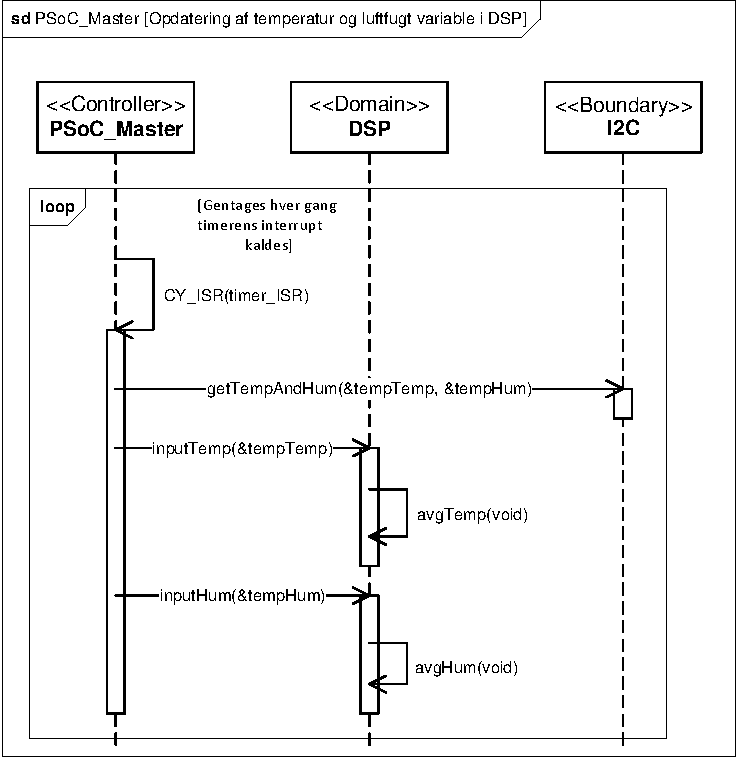
\includegraphics[scale=1]{../fig/sd_PSoC_master_update_sensor_values}
\caption{Sekvensdiagram over opdatering af sensorer.}
\label{fig:sd_PSoC_master_sensor}
\end{figure}

\begin{figure}[h]
\centering
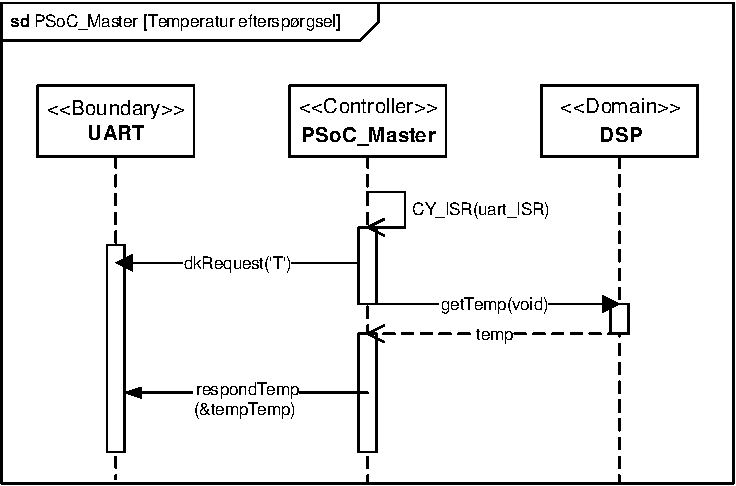
\includegraphics[scale=1]{../fig/sd_PSoC_master_tempreq}
\caption{Sekvensdiagram over forespørgsel af temperatur.}
\label{fig:sd_PSoC_master_tempreq}
\end{figure}

\begin{figure}[h]
\centering
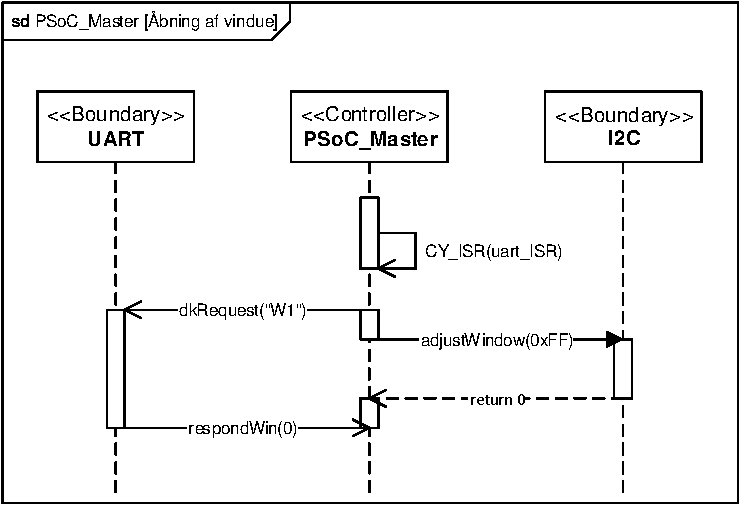
\includegraphics[scale=1]{../fig/sd_PSoC_master_open_window}
\caption{Sekvensdiagram over åbning af vindue.}
\label{fig:sd_PSoC_master_window}
\end{figure}



\clearpage
\section{Aktuator Design (Henrik og Morten)}

Dette afsnit omhandler design af blokken Aktuator. Den opdeles i underblokkene Varmelegeme, Blæsere, Vinduesmotor og PSoC4.

\subsection{Varmelegeme}

\begin{figure}[h]
\centering 
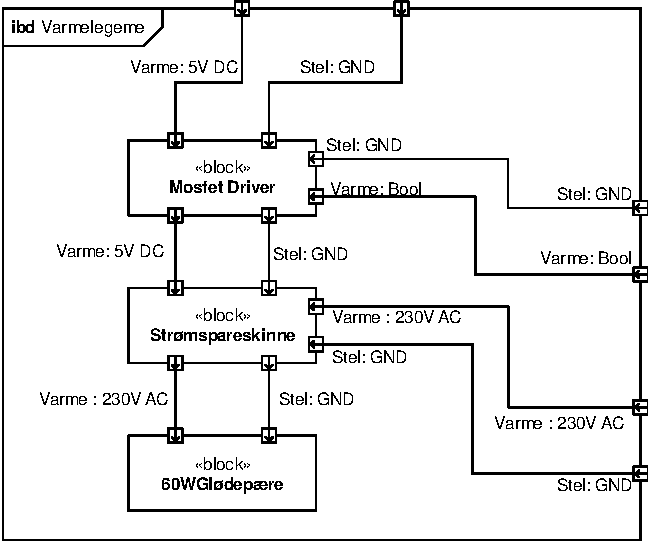
\includegraphics[width={\textwidth-5cm}, trim=0 0 0 0, clip=true] {../fig/ibd_varmelegeme.pdf}
\caption{IBD for underblokken Varmelegeme i Aktuator}
\label{fig:ibd_varmelegeme}
\end{figure}

Ovenstående diagram (Figur \ref{fig:ibd_varmelegeme}) viser interne forbindelser i underblokken Varmelegeme i Aktuator. 
For at undgå håndtering af 230V AC, består underblokken af en USB strømspareskinne, så selve varmelegemet (1-3 stk. 100W Glødepære) kan tændes og slukkes med et 5V DC signal. 
Antallet af tilkoblede glødepærer bestemmes under senere tests.

Aktuatorens SW er designet således at der nemt kan opgraderes til PWM styring af varmelegemet. 
Dette viser sig desværre at være umuligt med denne opstilling, da USB strømspareskinnen indeholder et mekanisk relæ; det er ikke muligt at opnå en frekvens hvor lyset ikke blinker. 
Dette vil sandsynligvis resultere i en sprunget glødepære.
En mulig løsning på problemet kunne være at tænde og slukke de 230V AC direkte med Mosfet transistoren, men vi må ikke håndtere så høje spændinger. 
En anden mulig løsning er at anvende for eksempel 12V glødepærer i stedet. Der skal dog nok temmelig mange til for at opnå samme effekt. 

Såfremt det senere vælges at opgradere til PWM styring, skal man tage højde for - eller se bort fra - at effekten ikke er lineært sammenhængende med dytucyclen. Dette skyldes dels at effekt har en sammenhæng med kvadratet af strømmen, dels at modstanden i glødetråden afhænger af temperaturen. 

\clearpage

\begin{figure}[h]
\centering 
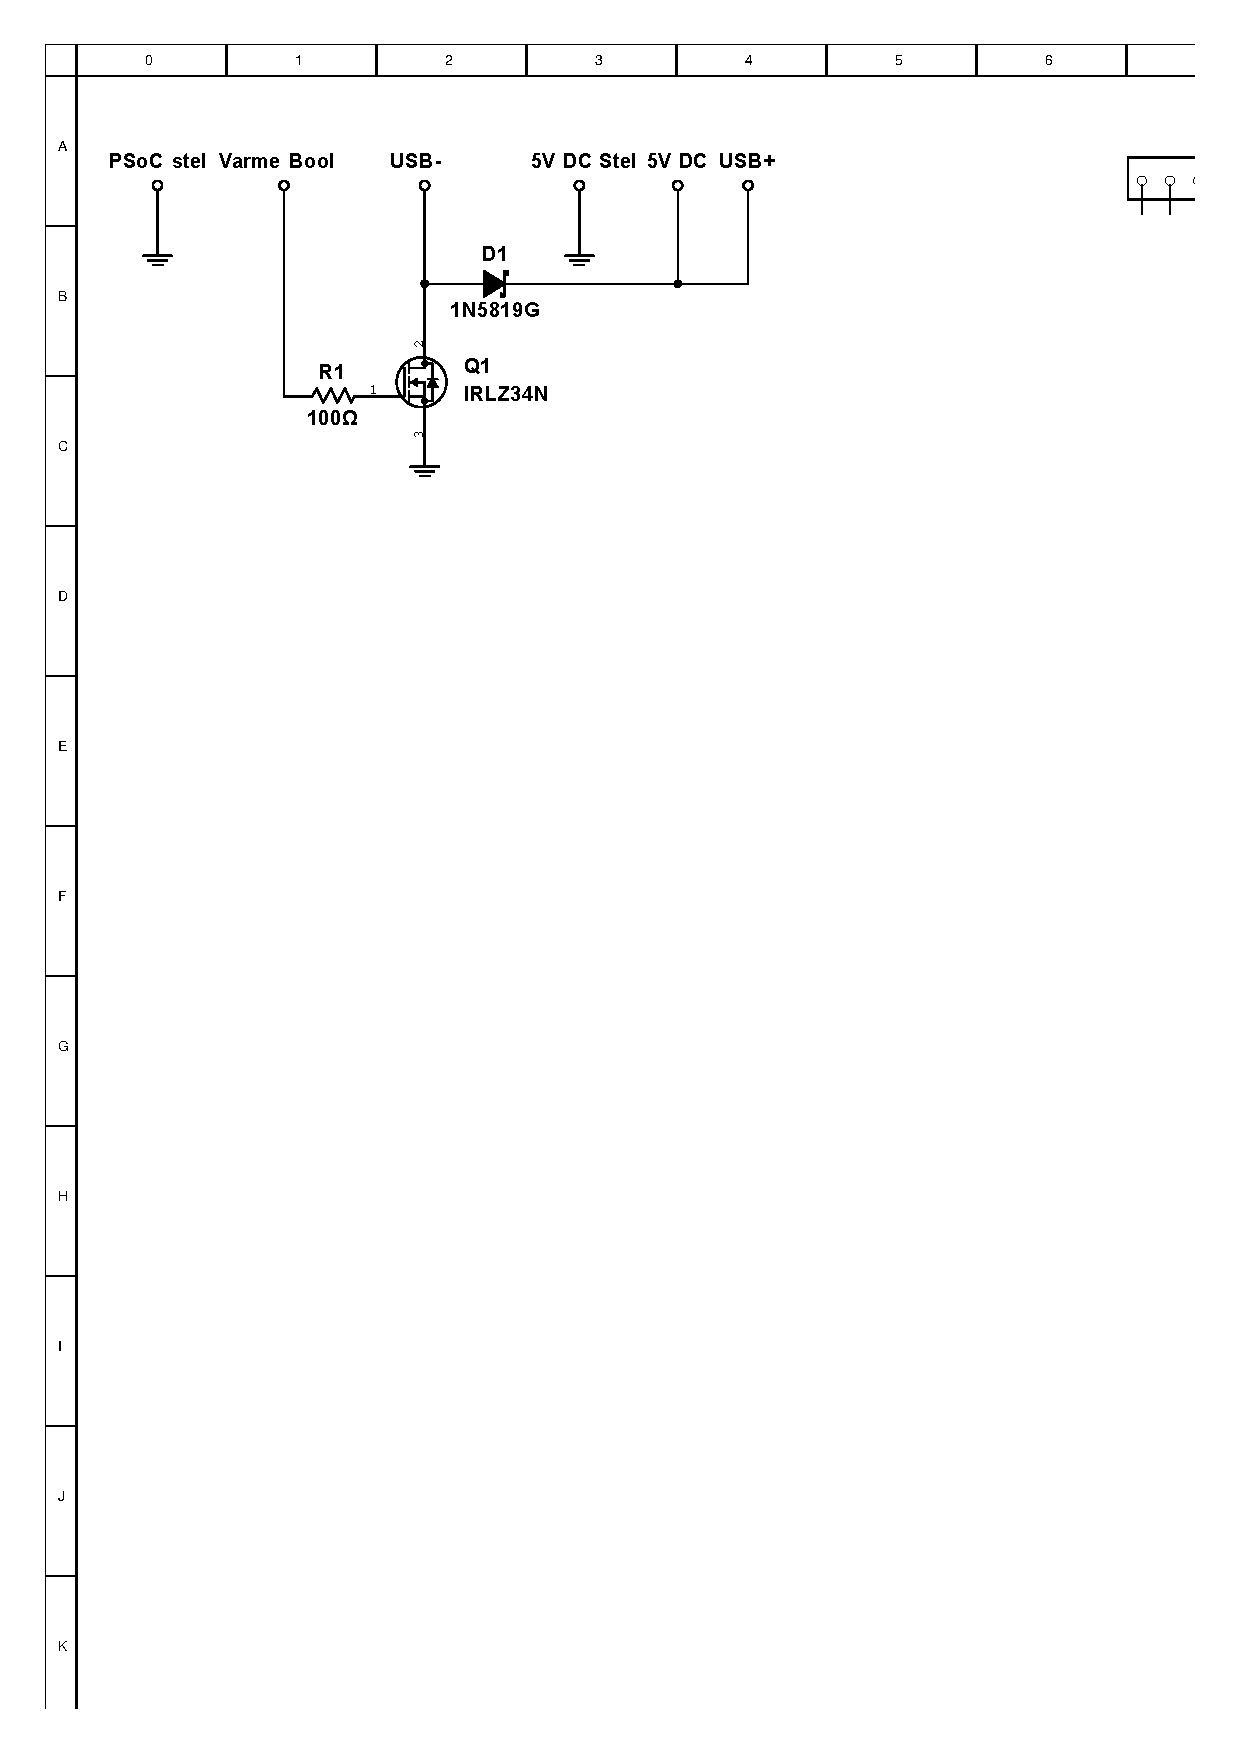
\includegraphics[width={\textwidth-5cm}, trim= 50 610 220 70, clip=true] {../fig/multisim_varmelegeme_mosfetdriver.pdf}
\caption{Kredsløb for Mosfet Driver i underblokken Varmelegeme}
\label{fig:multisim_varmelegeme_mosfetdriver}
\end{figure}

Når Varme Bool på Figur \ref{fig:ibd_varmelegeme} går høj, lukker mosfet transistoren, og tilslutter derved stel til USB Strømspareskinnen; varmelegemet forsynes med 230V AC. 
Når Varme Bool går lav, åbner mosfet transistoren, og derved afbrydes stel til Strømspareskinnen; varmelegemet forsynes ikke.  

D1 er er indsat for at sikre transistoren mod peakspændinger fra USB skinnen, når den slukkes. Dette er sandsynligvis ikke nødvendigt, men da vi ikke har indblik i hvordan USB strømspareskinnen rent faktisk virker, er dioden indsat for en sikkerheds skyld. 

Modstanden R1 er en beskyttelsesmodstand, som beskytter PSoC4, hvis Mosfet transistoren brændes af. 

\clearpage

\subsection{Blæsere}

\begin{figure}[h]
\centering 
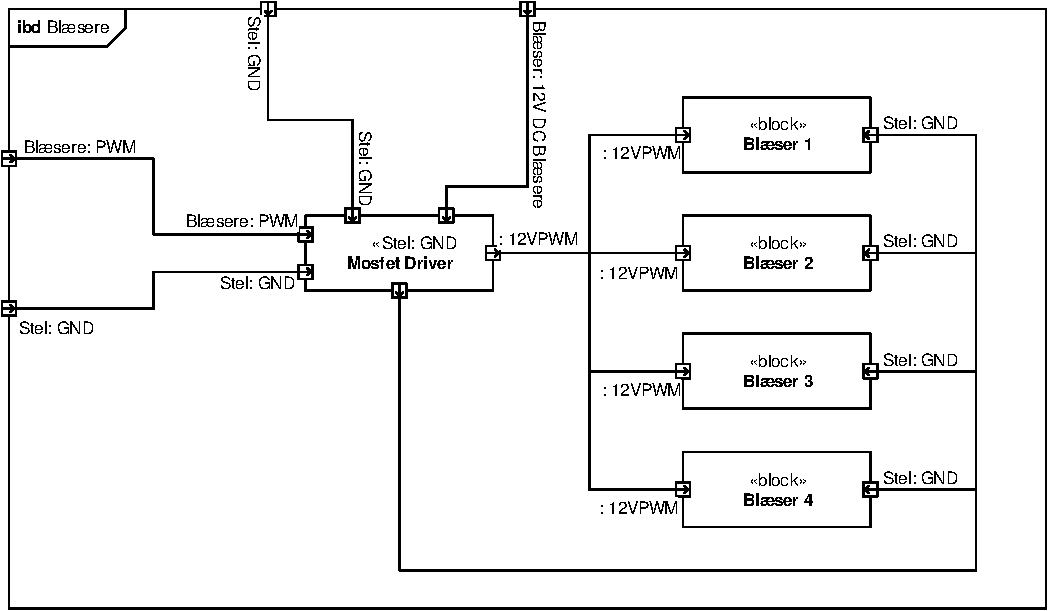
\includegraphics[width={\textwidth}, trim=0 0 0 0, clip=true] {../fig/ibd_blaesere.pdf}
\caption{IBD for underblokken Blæsere i Aktuator}
\label{fig:ibd_blaesere}
\end{figure}

Figur \ref{fig:ibd_blaesere} viser interne forbindelser i underblokken Blæsere, der består af en Mosfet Driver og fire 12V blæsere. 
To af blæserne er monteret således at luft blæses ind i drivhuset, mens de to øvrige blæsere blæser luft ud af drivhuset. 
Det forventes at en dutycycle på 100\% udskifter al luft i drivhuset på meget kort tid; dutycyclen for 'tændte blæsere' bestemmes ved praktiske forsøg under realisering af underblokken. 

Ved praktiske forsøg, konstateredes det, at en dutycyce på 50\% er et fornuftigt maximum. Det konstateredes desuden, at blæserne skal startes på maximum (dutycycle 50\%) for at komme i gang. 
Hvis der startes med en mindre dutycycle, opnår motoren ikke inerti nok til at begynde dreje. 
Begge dele implementeres i SW. 

\clearpage
 
\begin{figure}[h]
\centering 
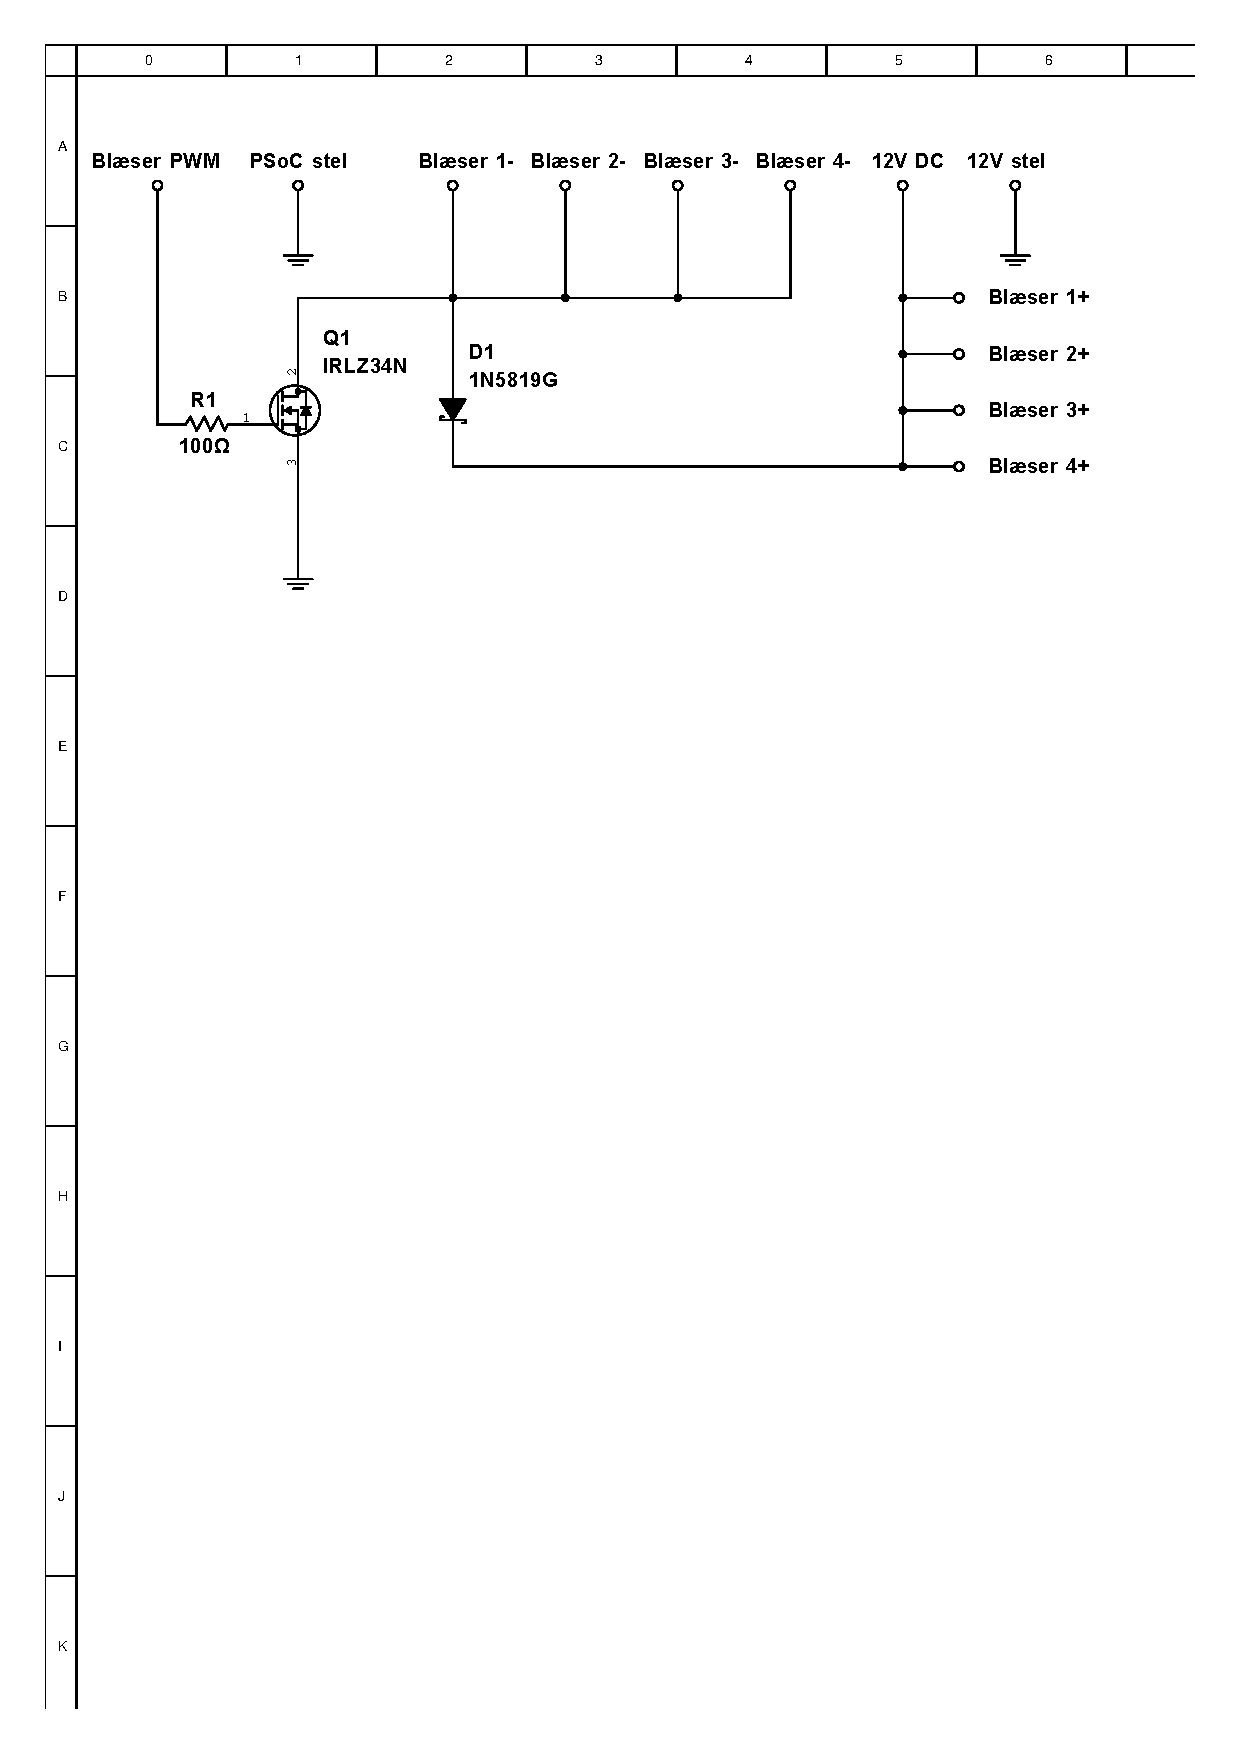
\includegraphics[width={\textwidth}, trim= 40 550 70 70, clip=true] {../fig/multisim_blaesere_mosfetdriver.pdf}
\caption{Kredsløb for Mosfet Driver i underblokken Blæsere}
\label{fig:multisim_blaesere_mosfetdriver}
\end{figure}

Mosfet Driveren til Blæsere på Figur \ref{fig:multisim_blaesere_mosfetdriver} fungerer i princippet på samme måde som Mosfet Driver for Varmelegeme (Figur \ref{fig:multisim_varmelegeme_mosfetdriver}).
Der er blot tilsluttet fire blæsere, der alle styres vha. den samme transistor. 

\clearpage

\subsection{Vinduesmotor}

\begin{figure}[h]
\centering 
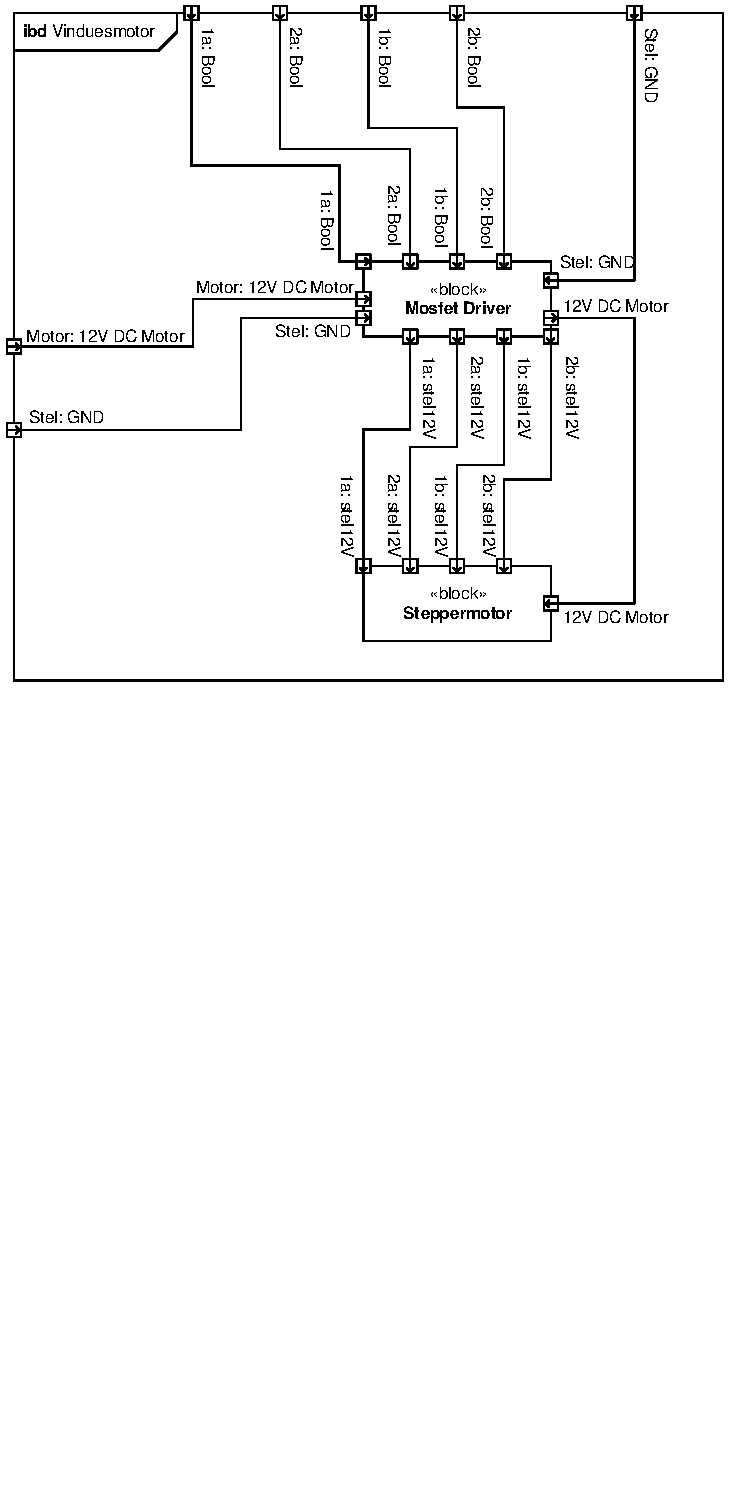
\includegraphics[width={\textwidth}, trim=0 390 0 0, clip=true] {../fig/ibd_vinduesmotor.pdf}
\caption{IBD for underblokken Vinduesmotor i Aktuator}
\label{fig:ibd_vinduesmotor}
\end{figure}

Ovenstående diagram (Figur \ref{fig:ibd_vinduesmotor}) viser interne forbindelser i underblokken Vinduesmotor, der består af en Steppermotor og en Mosfetdriver. 
Der åbnes og lukkes for mosfet transistorer i Mosfet Driveren vha. 3,3V signaler fra PSoC4, og derved forsynes Steppermotor med 12V DC. 
\\\\
Mosfet Driveren til Vinduesmotor på Figur \ref{fig:multisim_vinduesmotor_mosfetdriver} side \pageref{fig:multisim_vinduesmotor_mosfetdriver} fungerer i princippet på samme måde som Mosfet Driver for Blæsere (Figur \ref{fig:multisim_blaesere_mosfetdriver}).
Der er dog den forskel, at de fire signaler styres af hver deres transistor, da de ikke alle skal åbne og lukke samtidigt. 

\begin{figure}[h]
\centering 
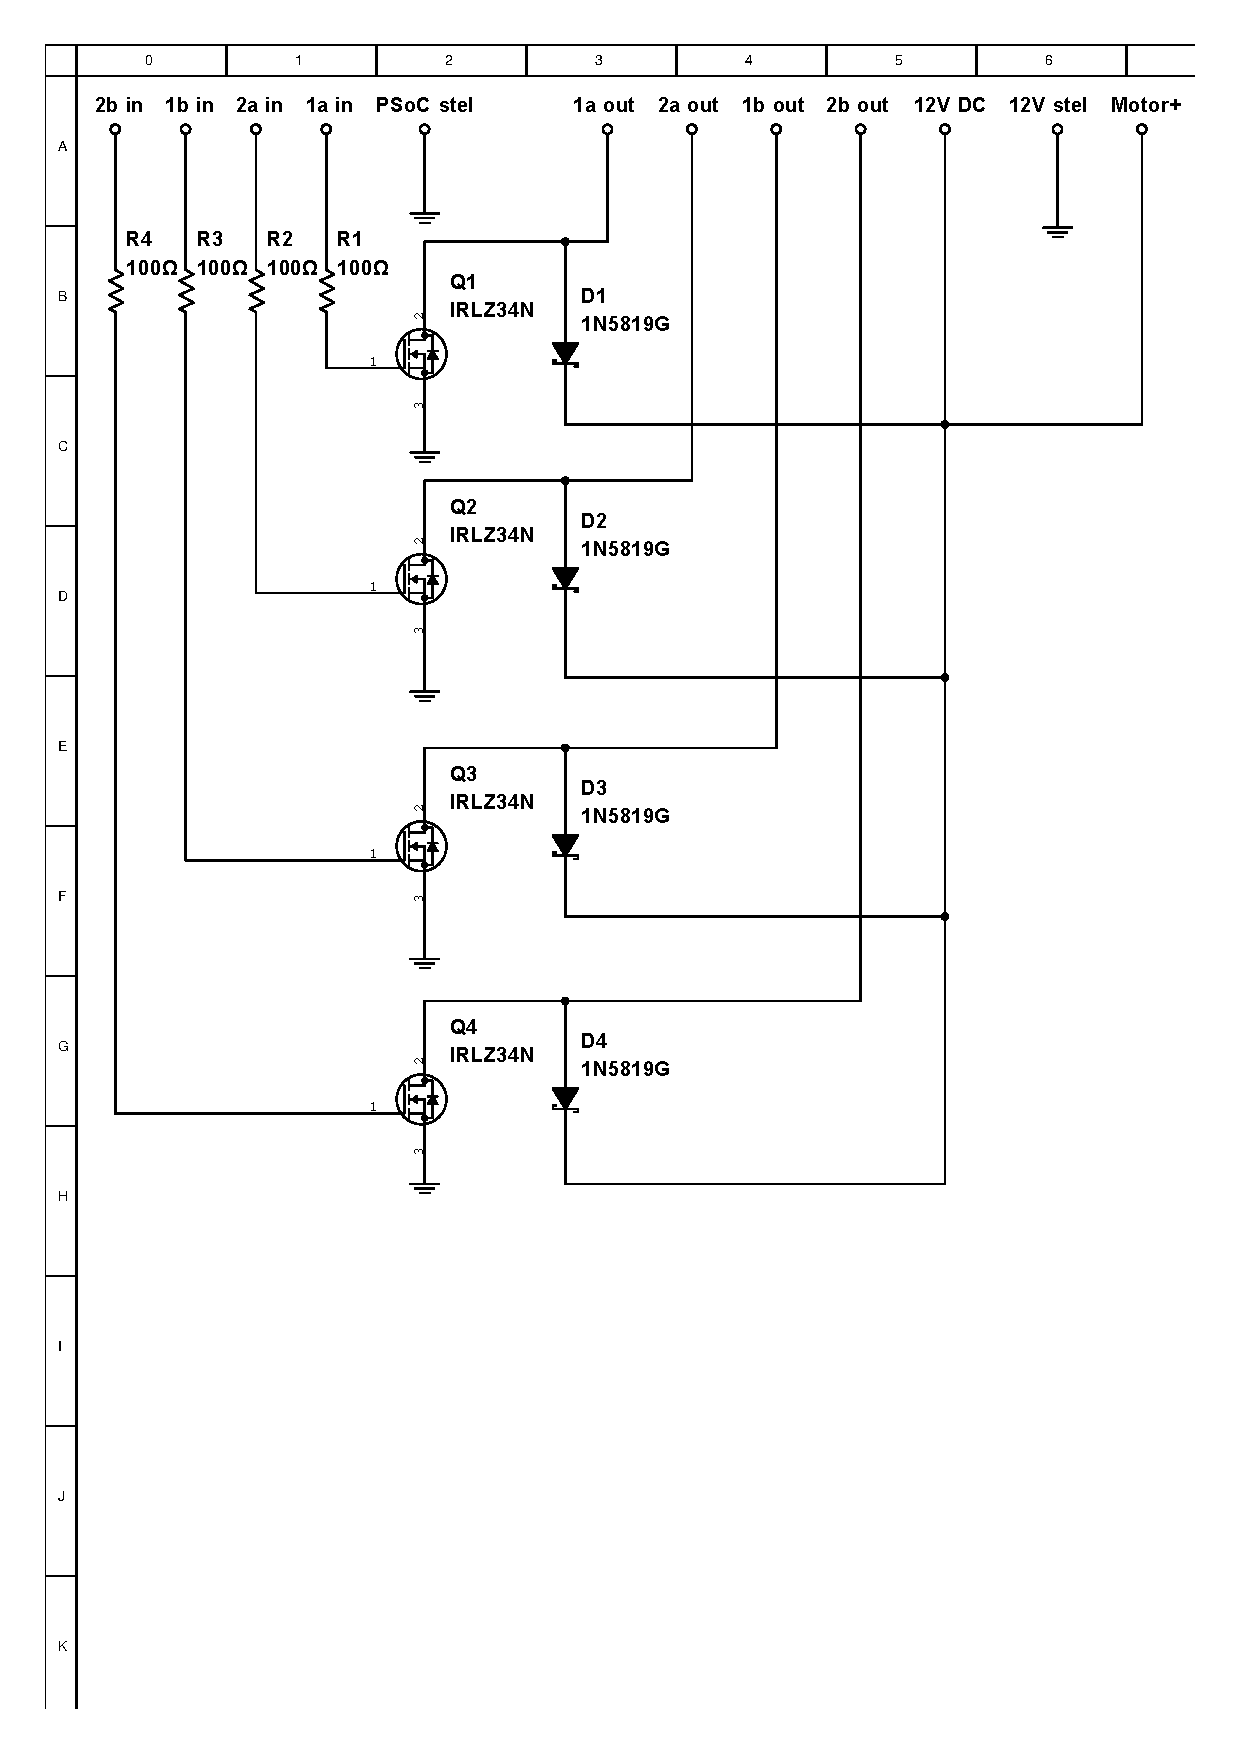
\includegraphics[width={\textwidth}, trim= 40 260 0 40, clip=true] {../fig/multisim_vinduesmotor_mosfetdriver.pdf}
\caption{Kredsløb for Mosfet Driver i underblokken Vinduesmotor}
\label{fig:multisim_vinduesmotor_mosfetdriver}
\end{figure}

\clearpage

\subsection{PSoC4}

\begin{figure}[h]
\centering 
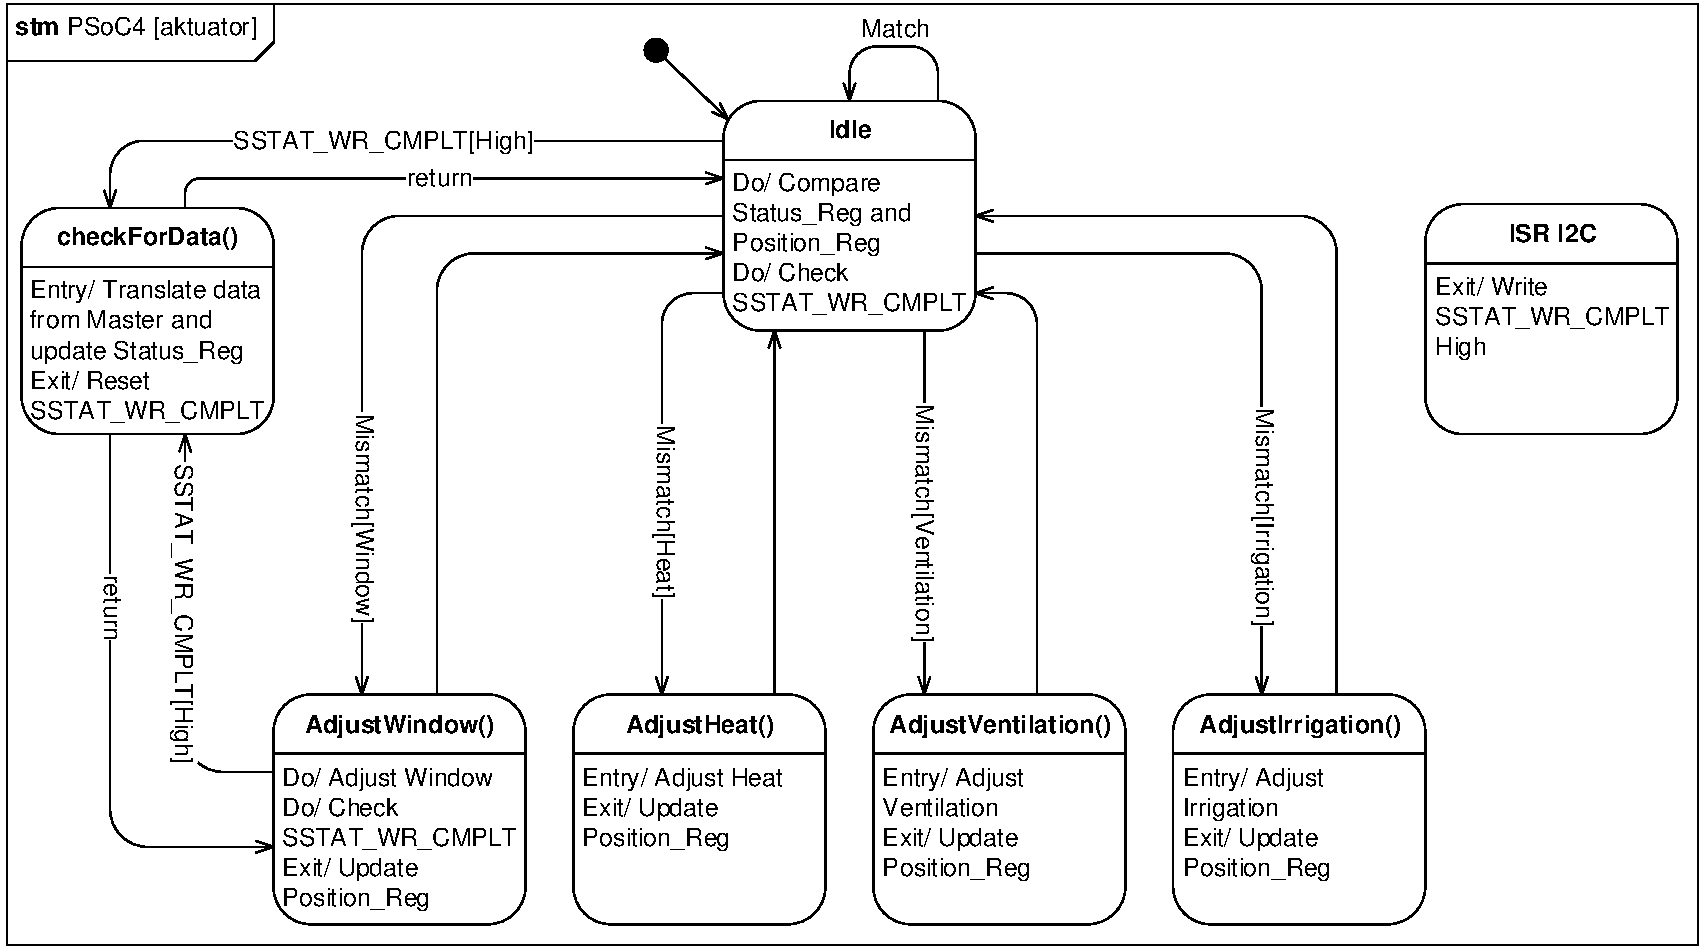
\includegraphics[width={\textwidth}, trim=0 0 0 0, clip=true] {../fig/stm_psoc_aktuator.pdf}
\caption{State Machine for software på underblokken PSoC4 i Aktuator}
\label{fig:stm_psoc_aktuator}
\end{figure}

Ovenstående diagram (Figur \ref{fig:stm_psoc_aktuator}) viser en state machine for software i underblokken PSoC4 i blokken Aktuator. 

Koden gentager tjek af om ønsket indstilling, af aktuatorer stemmer overens med aktuatorernes aktuelle indstilling og retter dette, såfremt det ikke er tilfældet. 
Denne rutine kan til enhver tid afbrydes af interrupt fra I2C bussen, der opdaterer slave write complete registeret (SSTAT\_WR\_CMPLT) fra lav til høj. Dette medfører at checkForData aktiveres som opdaterer ønskede indstillinger af aktuatorer. Herefter vil rutinen genoptages.
 
Ønskede indstillinger er gemt i registret Status\_Reg, mens aktuelle indstillinger er gemt i Position\_Reg.
 
Ved opdaterering af aktuatorer er den priorterede rækkefølge: Varme, blæsere, vanding og vindue. 
Vinduet er sidst i rækkefølgen, da det tager lang tid at åbne eller lukke. Koden for åbning eller lukning af vindue skrives således, at slave write complete registeret løbende tjekkes. Hvis dette register er højt vil indstillinger af aktuatorer opdateres, og derefter fortsætte fra vinduets position med de nye indstillinger.
Derved undgås det, at vinduet fx skal lukke helt, inden det åbnes, hvis disse to kommandoer modtages med meget kort mellemrum. 

\subsection{Drivers til PSoC4}
Dette afsnit beskriver drivere for opdatering af aktuatorer. 
Disse drivere er opdelt i Varme, Blæsere, Vanding, Vinduesmotor og checkForData. 
Derved kan systemet nemt opdateres, hvis der ændres på styringen af en bestemt aktuator. 
Alle drivere består af en header fil med prototyper og en source fil med implementeringer.

\subsubsection{Driver Varme}
Denne driver indeholder en funktionalitet, der har til formål at tænde eller slukke varmelegemet, samt opdatere aktuatorens bits i Position\_Reg. 
Dette sker ved at sætte en pin på PSoC4 hhv. høj eller lav; det gøres vha. PWM, da der så senere er nem mulighed for at opgradere styringen af varmelegemet til PWM styring. 

\subsubsection{Driver Blæsere}
Driveren for Blæsere har til formål at starte eller stoppe de fire blæsere i drivhuset, samt opdatere aktuatorens bits i Position\_Reg.
Dette sker ved at sende et PWM signal ud på en pin på PSoC4. 

\subsubsection{Driver Vanding}
Denne driver har til formål at aktivere eller deaktivere aktuatorer for vanding, samt opdatere aktuatorens bits i Position\_Reg. 
Dette sker ved at sætte 6 forskellige pins på PSoC4 hhv. høj eller lav. 

\subsubsection{Driver Vinduesmotor}
Driveren for vinduesmotoren har til formål at åbne eller lukke vinduet, samt opdatere aktuatorens bits i Position\_Reg. 
Antallet af omdrejninger for at åbne vinduet bestemmes under realisering ved praktiske forsøg. 
Driveren skal sammenligne Position\_Reg med Status\_Reg for hver omgang steppermotoren kører. 
Derved undgås det fx, at vinduet er nødt til at åbne helt inden det lukkes, hvis disse to kommandoer modtages hurtigt efter hinanden. 
Koden skrives således at det er nemt senere at opdatere driveren, så vinduet kan indstilles i flere trin mellem åbent og lukket. 

\subsubsection{Driver checkForData}
Denne driver har til formål at opdatere Status\_Reg. Der er mulighed for at kalde denne fra Idle tilstand og under AdjustWindow.
Driveren kaldes kun i det tilfælde, at I2C bussen har kaldt et interrupt, hvilket medfører opdatering af slave write complete registeret fra lav til høj.

\clearpage	
\section{Strømforsyning Design} \label{sec:Stroemforsyning_Design}

Som nævnt i systemarkitekturen forsyner strømforsyningen øvrig HW i systemet, undtagen selve varmelegemet og DevKit8000, der forsynes med 230V AC, og sensorerne, der forsynes med VEE (3.3V DC) fra PSoC Master.

Strømforsyningen forsynes med 12V DC max. 3A fra en laboratorieforsyning jf. Signalbeskrivelser på Tabel \ref{tbl:signalbeskriv} på side \pageref{tbl:signalbeskriv}. 
Alternativt kan anvendes en 12V transformer, der kobles til 230V AC. 

Strømforsyningen skal have 12V DC udgange til motor og blæsere, USB udgange med VDD til PSoC4 Pioneer Kits og en VDD udgang til USB strømspareskinnen.

\begin{figure}[h]
\centering 
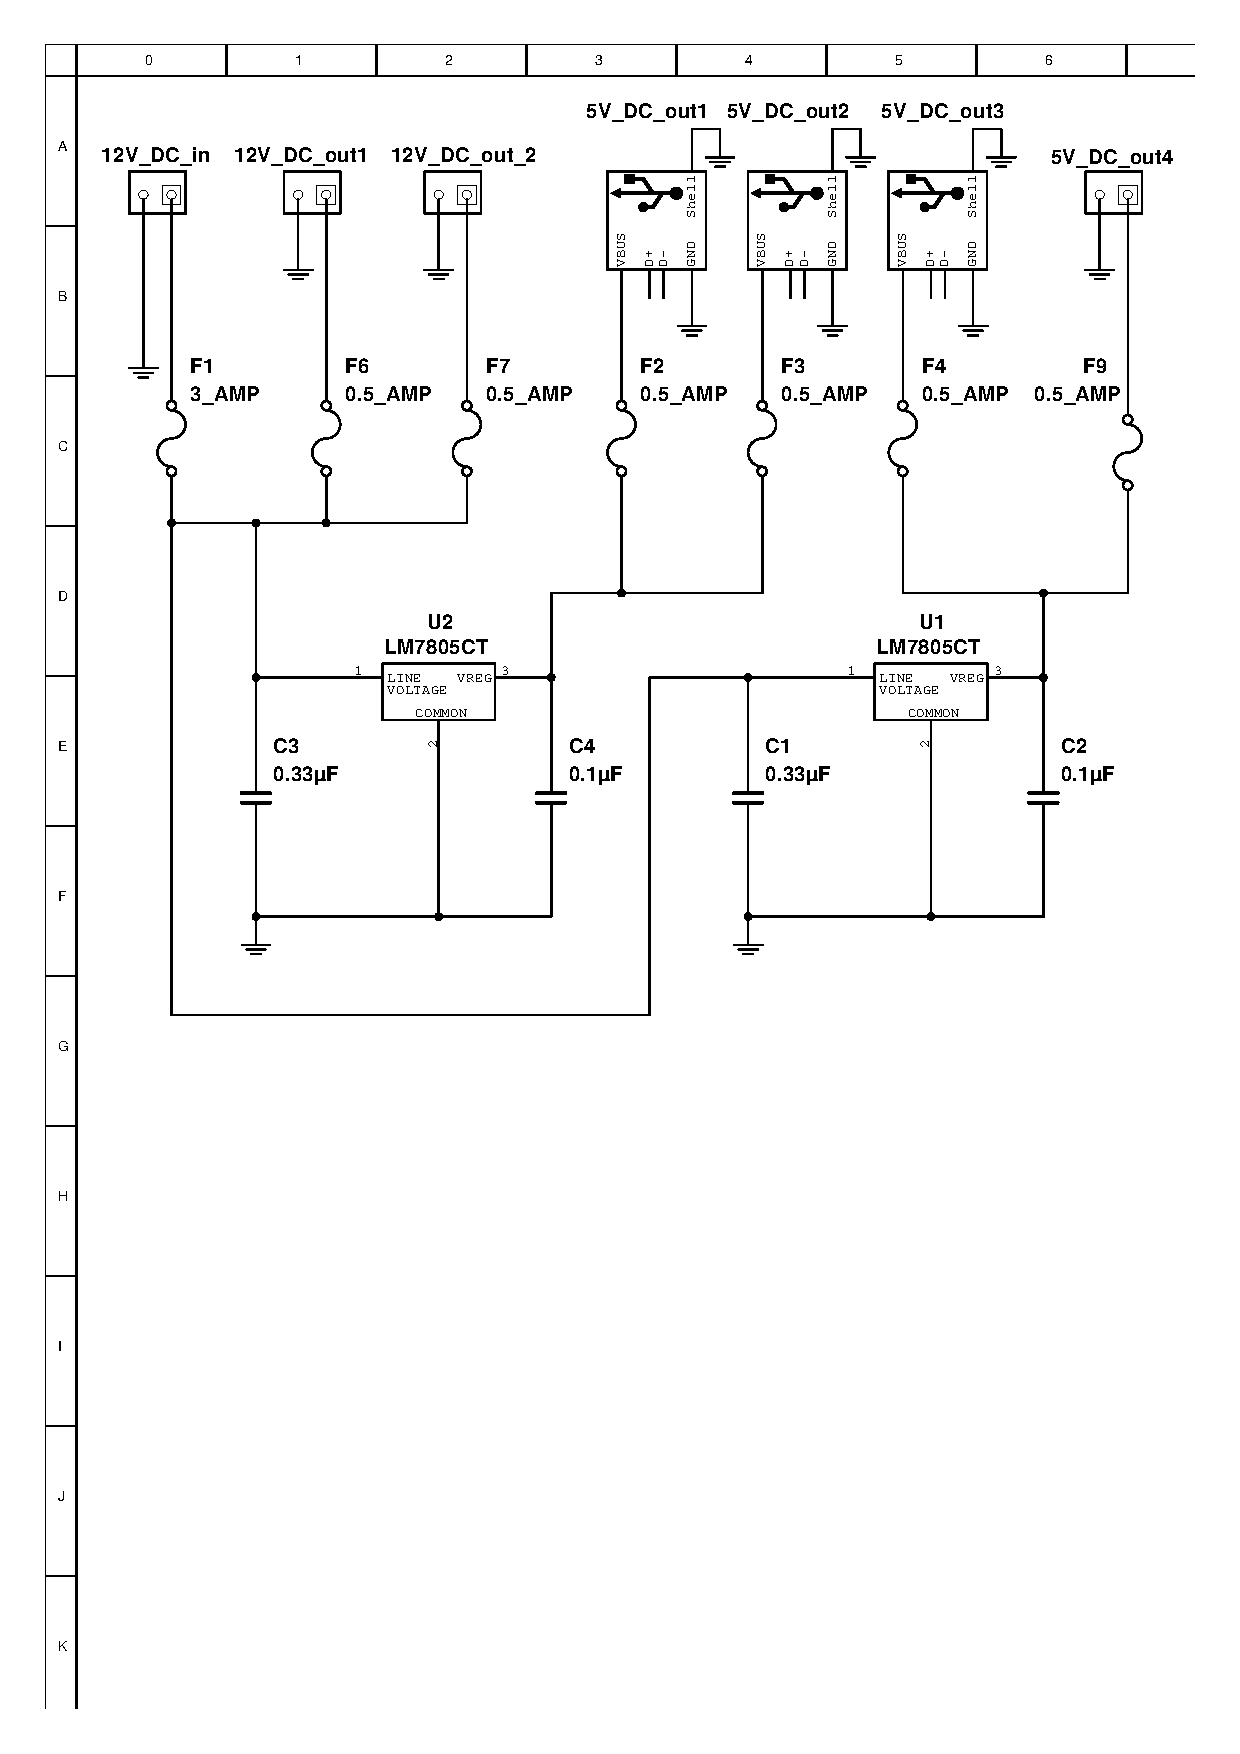
\includegraphics[width={\textwidth}, trim=50 350 30 40, clip=true] {../fig/multisim_stroemforsyning.pdf}
\caption{Diagram for blokken Strømforsyning}
\label{fig:multisim_stroemforsyning}
\end{figure}

Figur \ref{fig:multisim_stroemforsyning} viser Multisim diagram for designet af blokken Stroemforsyning. 
De enkelte komponenter og overvejelser herom gennemgås nedfor. 

\clearpage

12V DC in (VCC) trækker som sagt max. 3A, derfor monteres denne med en sikring på denne størrelse. 

12V DC out1 udgangen til motor trækker max. 500 mA jf. databladet \cite{lib:UHD2_DS} side 38, derfor monteres den med en sikring på 500 mA. 

De fire blæsere trækker hver især max. 140 mA ved fuld styrke jf. påtrykt værdi på selve blæserne. 
Implementeringen af koden i blokken Aktuator er lavet således, at blæserne maximalt kommer til at køre med en dutycycle på 50\%. 
Derfor monteres ligeledes en sikring på 500 mA til de fire blæsere. 

Ved en praktisk undersøgelse af USB skinnen konstateredes det, at USB indgangen trækker ca. 400 mA, når relæet er slået til, derfor monteres der også en 500 mA sikring på denne udgang. 

Der anvendes to spændingregulatorer LM7805, som begrænser 12V DC til 5V DC. 
De kan hver især levere 1A, derfor anvendes to stk. 
De monteres med afkoblinger til stel på ben 1 og 3 jf. standardapplikationen på side 1 i databladet \cite{lib:LM7805_DS}.

\clearpage


\section{Jordfugt Design} \label{sec:Jordfugt_Design}

Dette afsnit omhandler design af blokken Jordfugt, der består af et PSoC4 Pioneer kit og 0-6 jordfugtsensorer. 

\begin{figure}[h]
\centering 
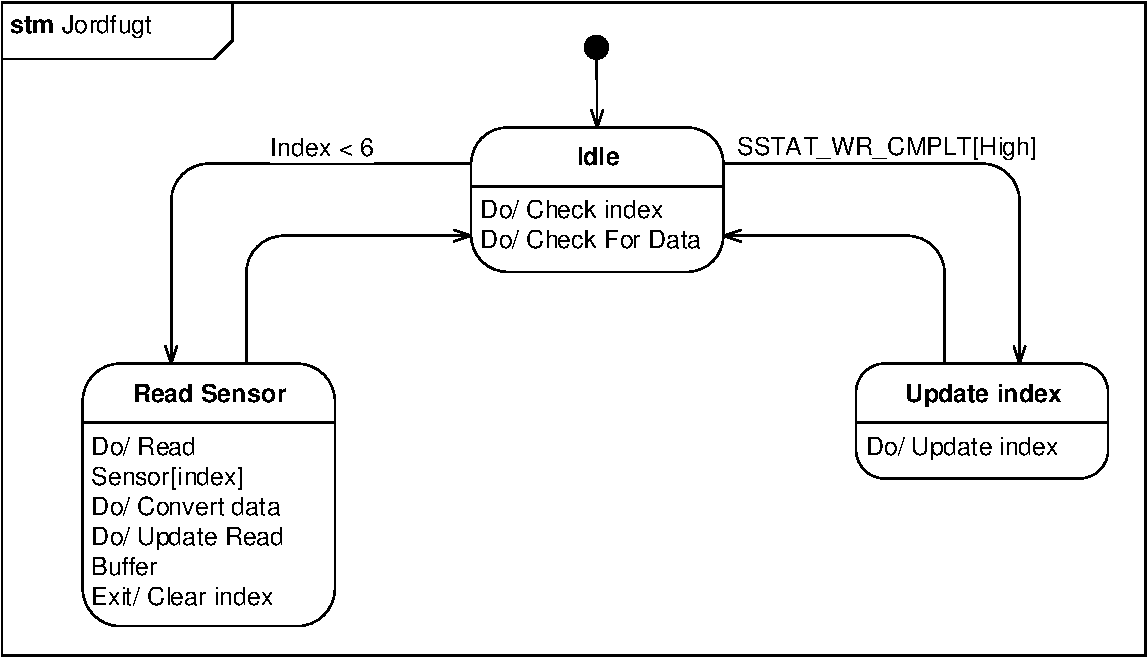
\includegraphics[width={\textwidth}, trim=0 0 0 0, clip=true] {../fig/stm_jordfugt.pdf}
\caption{State Machine for SW på PSoC4 i blokken Jordfugt}
\label{fig:stm_jordfugt}
\end{figure}

Ovenstående figur (Figur \ref{fig:stm_jordfugt}) viser en state machine for SW i PSoC4 i blokken Jordfugt.
 
PSoC'en står hele tiden og poller på om der er modtaget data, og om en indexvariabel er mindre end 6, som er det maximale antal jordfugtsensorer, der kan tilkobles.

Såfremt der er modtaget data via \IIC komminukationen, opdateres index variablen til det sensornummer, der er modtaget. 

Såfremt index variablem er mindre end 6, læses der på den tilhørende sensor, data konverteres til et tal mellem 1 - 100, og read bufferen opdateres med den læste værdi. 

\mbox{}

Der er i forbindelse med brugen af sensoren lavet en støjundersøgelse i faget Mixed Signal Elektronik. 
Se journalen \cite{lib:MSE_06} for nærmere info. 
I AutoGreen anvendes jordfugtsensoren på en noget simplere måde end i øvelsen, se afsnittet om implementering af blokken Jordfugt for nærmere info.

\clearpage
%TODO SoftwareDesign?
\chapter{Hardware Implementering}

\section{Version}
\begin{table}[h]
	\centering
	\begin{tabularx}{\textwidth - 2cm}{|l|l|l|X|}
	\hline
	Dato	& Version	& Initialer & Ændring	\\ \hline
	31. marts & 1 & MHG & Implementering af SW i Aktuator. \\ \hline
	8. april & 2 & MHG & Færdiggjort beskrivelse af SW i Aktuator. \\\hline
	\end{tabularx}
\end{table}

%\section{Aktuator} \label{sec:AktImpl}

Dette afsnit beskriver implementering af SW og HW i blokken Aktuator. Afsnittet beskriver først hhv. HW og SW i underblokken PSoC4, herefter HW i underblokkene Varmelegeme, Blæsere og Vinduesmotor.

\subsection{HW PSoC4}
\begin{figure}[h]
\centering 
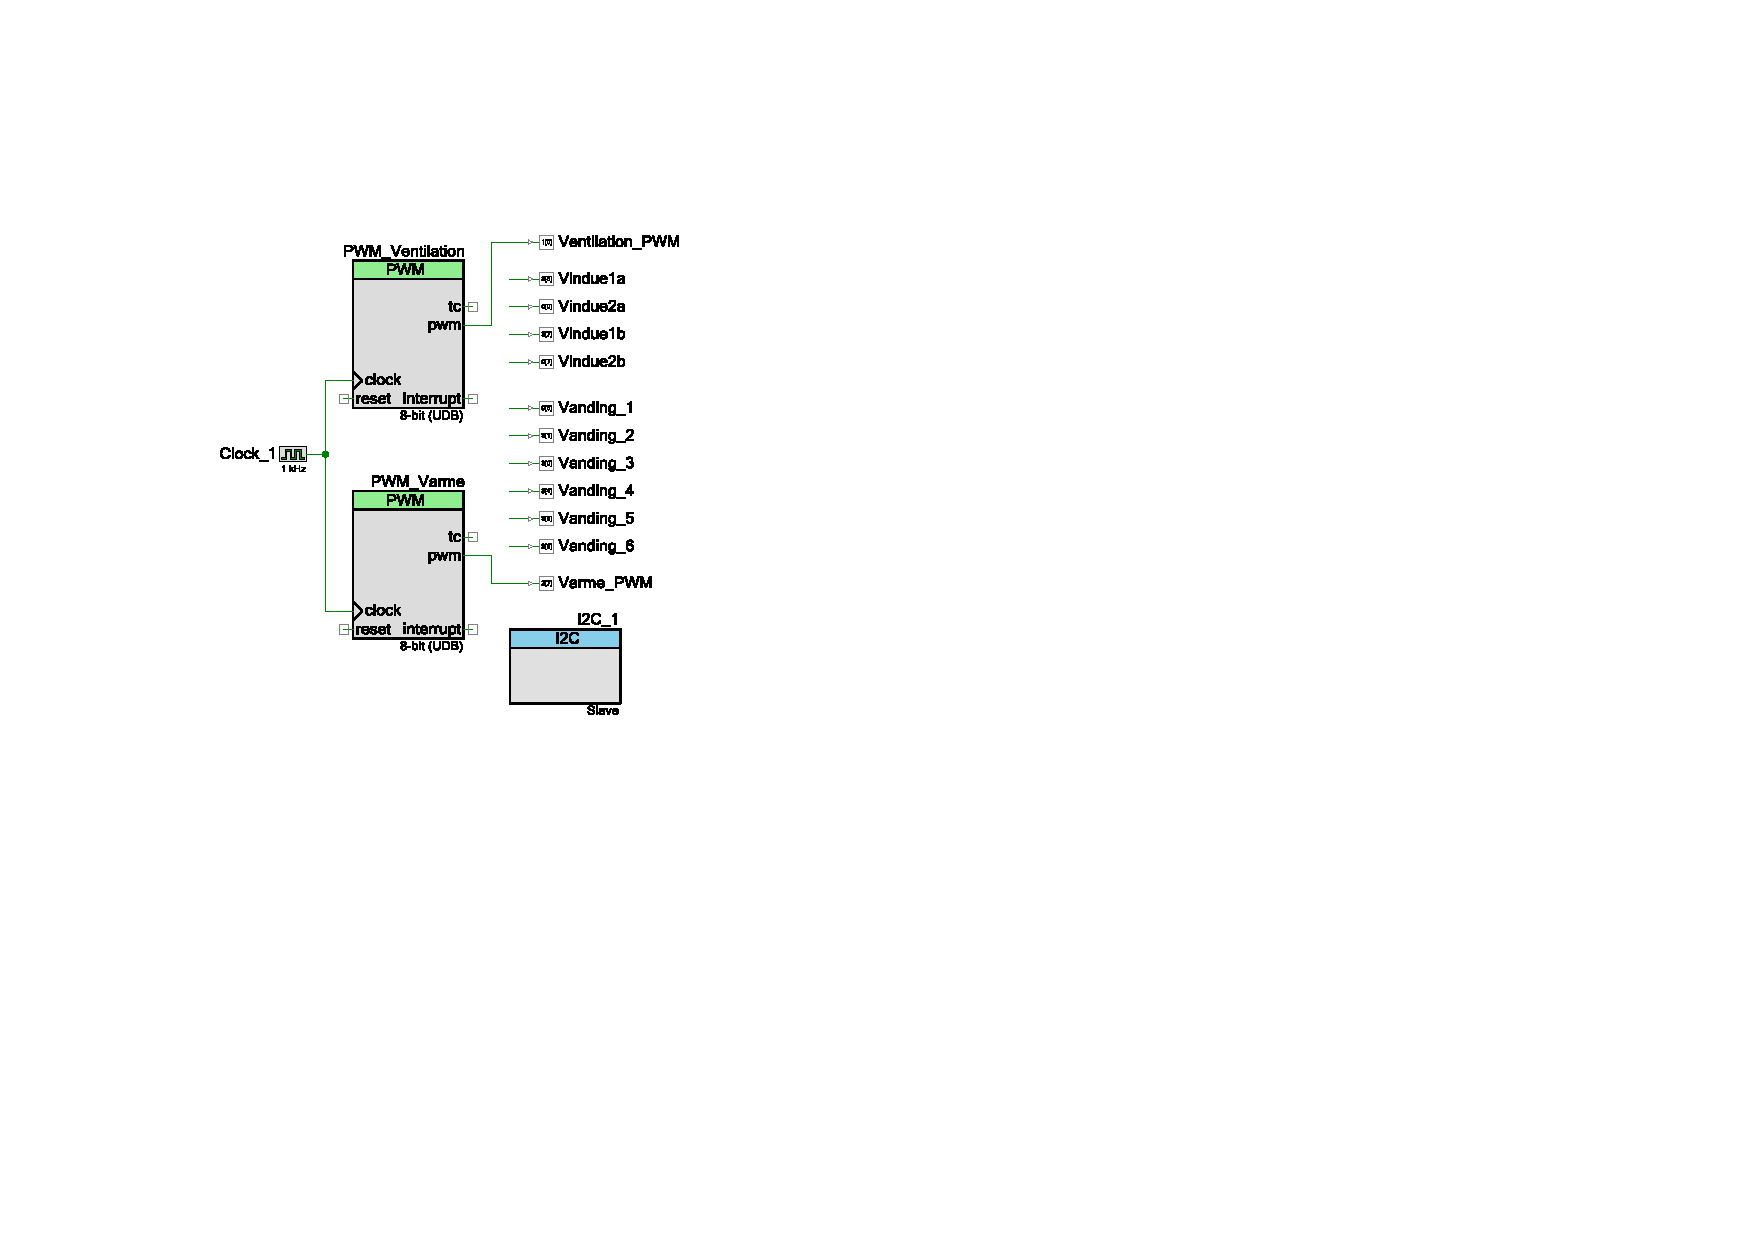
\includegraphics[width={\textwidth-6cm}, trim = 110 320 480 100, clip=true] {../fig/TopDesign_Aktuator.pdf}
\caption{TopDesign.cysch for PSoC4 i Aktuator}
\label{fig:topdesign_aktuator}
\end{figure}

Den HW, der syntetiseres i PSoC4 Aktuator er vist på figur\ref{fig:topdesign_aktuator}. 

Clock\_1 forsyner PWM komponenten med en grundfrekvens; der er valgt 1 kHz.

PWM\_Ventilation genererer et PWM signal til styring af drivhusets fire ventilatorer. Timeren er indstillet til 8 bit.  

I2C\_1 komponenten styrer kommunikation med MasterPSoC via \IIC. 
Den konfigureret til at være slave med adressen 0x42, datarate er indstillet til 100 kbps.

Alle pins i topdeignet er konfigureret til strong drive. 
Det vil sige at de altd er defineret enten high eller low.

\clearpage

\subsection{SW PSoC4}

\begin{lstlisting}[caption=Udsnit af main.c for PSoC4 i Aktuator, label=fig:main_aktuator]
    for(;;) //Evigt loop
    {
        checkForData(); //Opdater Status_Reg, hvis der er modtaget data
        
        if(!(Status_Reg == Position_Reg))//Hvis der er et mismatch
        {
            //Tjek for mismatch for Varme
            if(!((Status_Reg & 0b0000111000000000) == (Position_Reg & 0b0000111000000000)))
            {
                AdjustHeat();
            }
            
            //Tjek for mismatch for Ventilation
            if(!((Status_Reg & 0b0000000111000000) == (Position_Reg & 0b0000000111000000)))
            {
                AdjustVentilation();
            }
            
            //Tjek for mismatch for Vanding
            if(!((Status_Reg & 0b0000000000111111) == (Position_Reg & 0b0000000000111111)))
            {
                AdjustIrrigation();
            }
            
            //Tjek for mismatch for Vindue
            if(!((Status_Reg & 0b1111000000000000) == (Position_Reg & 0b1111000000000000)))
            {
                AdjustWindow();
            }
        }
    }
\end{lstlisting}

Filen main.c, hvoraf den vigtigste del er vist på Listing \ref{fig:main_aktuator}, fungerer jf. State Machinen på Figur \ref{fig:stm_psoc_aktuator} side \pageref{fig:stm_psoc_aktuator}.

Programmet tjekker om der er modtaget data på \IIC, og opdaterer evt. ønskede indstillinger for aktuatorer i Status\_Reg. 

Herefter sammenlignes Status\_Reg med nuværende indstillinger af aktuatorer i Position\_Reg.

Såfremt der er uoverensstemmelse, opdateres den pågældende aktuator. 

Sammenligningen af de to registre sker i en prioriteret rækkefølge. 

Vinduet er sidste i denne proces, da det tager temmelig lang tid (flere sekunder) at åbne eller lukke vindet. 

\clearpage

\begin{lstlisting}[caption=Udsnit af checkForData.c for PSoC4 i Aktuator, label=fig:checkForData_aktuator]
void checkForData()
{
    uint16 temp = 0;
    //Check for om der er modtaget data
    if(I2C_1_I2CSlaveStatus() & I2C_1_I2C_SSTAT_WR_CMPLT)
    {
        //Put data i Status_Reg            
        if((writeBuffer[0] >> 6) == 0x0) //Check for Vindue
        {
            //Put data fra buffer i uint16 og skift til rigtig position
            temp = (writeBuffer[0] & 0b00001111) << 12; 
            //Overskriv relevante pladser med 0'er
            Status_Reg = Status_Reg & 0b0000111111111111;
            //Put nye data ind i Status_Reg
            Status_Reg = Status_Reg | temp;                
        }           
        if((writeBuffer[0] >> 6) == 0x1) //Check for Varme
        {
            //Put data fra buffer i uint16 og skift til rigtig position
            temp = (writeBuffer[0] & 0b00000111) << 9; 
            //Overskriv relevante pladser med 0'er
            Status_Reg = Status_Reg & 0b1111000111111111;
            //Put nye data ind i Status_Reg
            Status_Reg = Status_Reg | temp;                
        }           
        if((writeBuffer[0] >> 6) == 0x2) //Check for Ventilation
        {
            //Put data fra buffer i uint16 og skift til rigtig position
            temp = (writeBuffer[0] & 0b00000111) << 6; 
            //Overskriv relevante pladser med 0'er
            Status_Reg = Status_Reg & 0b1111111000111111;
            //Put nye data ind i Status_Reg
            Status_Reg = Status_Reg | temp;                
        }            
        if((writeBuffer[0] >> 6) == 0x3) //Check for Vanding
        {
            //Put data fra buffer i uint16 og skift til rigtig position
            temp = (writeBuffer[0] & 0b00111111); 
            //Overskriv relevante pladser med 0'er
            Status_Reg = Status_Reg & 0b1111111111000000;
            //Put nye data ind i Status_Reg
            Status_Reg = Status_Reg | temp;                
        }                    
        I2C_1_I2CSlaveClearWriteBuf(); //Clear buffer pointer
        I2C_1_I2CSlaveClearWriteStatus(); //Clear status                       
        //Opdater Read buffer
        readBuffer[0] = Status_Reg >> 8;
        readBuffer[1] = Status_Reg;     
        I2C_1_I2CSlaveClearReadBuf();
    }
}
\end{lstlisting}

\clearpage

Funktionen checkForData() på Listing \ref{fig:checkForData_aktuator} checker om slavens status er, at den har modtaget data. 

I så fald checker den for hvilken aktuator, der modtages data til.
Herefter behandles data, og Status\_Reg opdateres.

Efter dette klargøres systemet til at modtage nye data, ved at write buffer og status for slaven nulstilles.

Til slut opdateres read buffer, i tilfælde af at MasterPSoC beder om information om aktuel status. 
\newline
\begin{lstlisting}[caption=Udsnit af heat.c for PSoC4 i Aktuator, label=fig:heat_aktuator]
void InitHeat()
{   
    //Slukker for Varme
    Varme_Write(0);
    
    //Opdater nuvaerende indstillinger
    Position_Reg = Position_Reg & 0b1111000111111111;
}

void AdjustHeat()
{
    //Opdater aktuator for varmelegeme
    Varme_Write((Status_Reg & 0b0000111000000000) >> 9);
    
    //Opdater nuvaerende indstillinger
    Position_Reg = Position_Reg & 0b1111000111111111;
    Position_Reg = Position_Reg | (Status_Reg & 0b0000111000000000);
}
\end{lstlisting}

Koden i heat.c i Listing \ref{fig:heat_aktuator} består af to funktioner. 

InitHeat()trækker pin for varme lav og initialiserer indstilling af Position\_Reg for varme.

AdjustHeat() opdaterer pin for varme og Position\_Reg opdateres med de nuværende indtillinger for aktuator. 

\clearpage

\begin{lstlisting}[caption=Udsnit af ventilation.c for PSoC4 i Aktuator, label=fig:ventilation_aktuator]
void InitVentilation()
{
    //Start komponent
    PWM_Ventilation_Start();
    //Sluk ventilatorer
    PWM_Ventilation_WriteCompare(0);
    //Opdater nuvaerende indstillinger
    Position_Reg = Position_Reg & 0b1111111000111111;
}

void AdjustVentilation()
{
    //Start med fuld styrke for at blaeserne kommer i gang.
    PWM_Ventilation_WriteCompare((MAXIMUM_VENT*255)/100);
    CyDelay(100);
    //Omregn bits fra Status_Reg og start PWM med oensket dutycycle
    PWM_Ventilation_WriteCompare((((Status_Reg & 0b0000000111000000) >> 6)*MAXIMUM_VENT*255)/(7*100));
    
    //Opdater nuvaerende indstillinger
    Position_Reg = Position_Reg & 0b1111111000111111;
    Position_Reg = Position_Reg | (Status_Reg & 0b0000000111000000);
}
\end{lstlisting}

Koden i ventilation.c i Listing \ref{fig:ventilation_aktuator} består af to funktioner. 

InitVentilation() starter PWM komponenten, slukker for blæsere (dutycycle = 0\%) og initialiserer indstilling af Position\_Reg for ventilation.

AdjustVentilation() indstiller ønsket dutycycle i PWM komponenten. 

MAXIMUM\_VENT er en global definition af den dutycycle, der maximalt ønskes. Ved praktiske forsøg er det konstateret at 50\% er passende.

For at sikre at blæserne rent faktisk kommer i gang, startes PWM komponenten først for fuld styrke i 100 ms, hvorefter den ønskede dutycycle indstilles.

Der er som udgangspunkt kun mulighed for at tænde eller slukker for ventilationen, men ved at lave koden på denne måde, kan systemet meget nemt opgraderes, hvis PWM styring af varmelegemet ønskes. 

Efter start at PWM komponenten opdateres Position\_Reg med de nuværende indtillinger for aktuatorer.

\clearpage

\begin{lstlisting}[caption=Udsnit af irrigation.c for PSoC4 i Aktuator, label=fig:irrigation_aktuator]
void InitIrrigation()
{
    //Sluk for al vanding
    Vanding_1_Write(0);
    Vanding_2_Write(0);
    Vanding_3_Write(0);
    Vanding_4_Write(0);
    Vanding_5_Write(0);
    Vanding_6_Write(0);
    
    //Opdater nuvaerende indstillinger
    Position_Reg = Position_Reg & 0b1111111111000000;
}

void AdjustIrrigation()
{
    //Opdater alle aktuatorer for vanding
    Vanding_1_Write(Status_Reg & 0b0000000000000001);
    Vanding_2_Write((Status_Reg & 0b0000000000000010) >> 1);
    Vanding_3_Write((Status_Reg & 0b0000000000000100) >> 2);
    Vanding_4_Write((Status_Reg & 0b0000000000001000) >> 3);
    Vanding_5_Write((Status_Reg & 0b0000000000010000) >> 4);
    Vanding_6_Write((Status_Reg & 0b0000000000100000) >> 5);
    
    //Opdater nuvaerende indstillinger
    Position_Reg = Position_Reg & 0b1111111111000000;
    Position_Reg = Position_Reg | (Status_Reg & 0b0000000000111111);
}
\end{lstlisting}

Koden i irrigation.c i Listing \ref{fig:irrigation_aktuator} består af to funktioner. 

InitIrrigation() trækker alle pins for vanding lav og initialiserer Position\_Reg.

AdjustIrrigation() opdaterer alle pins for vanding og indstiller Position\_Reg.

\clearpage

\begin{lstlisting}[caption=Udsnit A af window.c for PSoC4 i Aktuator, label=fig:window1_aktuator]
void InitWindow()
{
    //Initialisering af pins til startposition
    Vindue1a_Write(1);
    Vindue2a_Write(1);
    Vindue1b_Write(0);
    Vindue2b_Write(0);
    //Initialisering af nuvaerende position
    currentTurn = 0;
    //Opdatering af nuvaerende indstillinger
    Position_Reg = Position_Reg & 0b0000111111111111;
}

void AdjustWindow()
{      
    //Konvertering af data fra Status_Reg og indsaettelse i desiredTurn.
    desiredTurn = ((MAX_WINDOW)*(((Status_Reg >> 12)*100)/15))/100;
    
    while(desiredTurn != currentTurn) //Saa laenge vinduet ikke er i oensket position
    {
        if (currentTurn > desiredTurn) //Luk 1 omgang hvis vinduet er for aabent
        {
            CloseOneTurn();
        }
    
        if (currentTurn < desiredTurn) //aaben 1 omgang hvis vinduet er for lukket
        {
            OpenOneTurn();
        }
    }
    //Opdatering af nuvaerende indstillinger
    Position_Reg = Position_Reg & 0b0000111111111111;
    Position_Reg = Position_Reg | (Status_Reg & 0b1111000000000000);
}
\end{lstlisting}

Kodeudnsnittet fra window.c på Listing \ref{fig:window1_aktuator} viser de to funktioner InitWindow() og AdjustWindow().

MAX\_WINDOW er en global definition, som angiver antallet af steps motoren skal køre, for at åbne vinduet helt. 
TIME\_BETWEEN\_STEPS er en global definition som angiver hvor mange milisekunder, der går mellem hvert af motorens steps. 
Ved praktiske forsøg er hhv. 420 steps og 10 ms fundet hensigtsmæssige.

InitWindow() initialiserer de fire vindues pins til startposition og initialiserer Position\_Reg. 

Den initialiserer desuden variablen currentTurn til 0. Denne variabel holder styr på hvor vinduet befinder sig. 

BEMÆRK! Vinduet skal være lukket, når systemet startes!

AdjustWindow() kontrollerer om currentTurn er større, mindre eller lig desiredTurn. Hvis de er forskellige kaldes enten OpenOneTurn() eller CloseOneTurn().

Herefter opdateres Position\_Reg.

\clearpage

\begin{lstlisting}[caption=Udsnit B af window.c for PSoC4 i Aktuator, label=fig:window2_aktuator]
void CloseOneTurn()//48 steps paa en omgang, 12*4=48, funktionen lukker 1/12 af en omgang.
{
    //Efter hvert fjerde step checkes der for ny data og stilling samt oenskede stilling opdateres
    Vindue1a_Write(0);
    Vindue2a_Write(1);
    Vindue1b_Write(1);
    Vindue2b_Write(0);
    CyDelay(TIME_BETWEEN_STEPS);
    Vindue1a_Write(0);
    Vindue2a_Write(0);
    Vindue1b_Write(1);
    Vindue2b_Write(1);
    CyDelay(TIME_BETWEEN_STEPS);
    Vindue1a_Write(1);
    Vindue2a_Write(0);
    Vindue1b_Write(0);
    Vindue2b_Write(1);
    CyDelay(TIME_BETWEEN_STEPS);
    Vindue1a_Write(1);
    Vindue2a_Write(1);
    Vindue1b_Write(0);
    Vindue2b_Write(0);
    CyDelay(TIME_BETWEEN_STEPS);
    checkForData();
    desiredTurn = ((MAX_WINDOW)*(((Status_Reg >> 12)*100)/15))/100;
    currentTurn--;
}

void OpenOneTurn()//48 steps paa en omgang, 12*4=48, funktionen aabner 1/12 af en omgang.
{
    ...
\end{lstlisting}

Kodeudnsnittet fra window.c på Listing \ref{fig:window2_aktuator} viser de to funktioner CloseOneTurn() (og OpenOneTurn()). 

CloseOneTurn() gennemløber sekvensen for at motoren kører et step mod urets retning.

Sekvensen i OpenOneTurn() er modsat, så motoren kører med urets retning. 

For hvert step motoren kører, tjekkes der for nye data, og desiredTurn opdateres. Dette sker for at en ny kommando til vinduet eksekveres inden en igangværende kommando afsluttes. Herefter opdateres currentTurn. Denne funktionalitet er implementeret i begge funktioner.

\clearpage

\subsection{HW Varmelegeme}

\begin{figure}[h]
\centering 
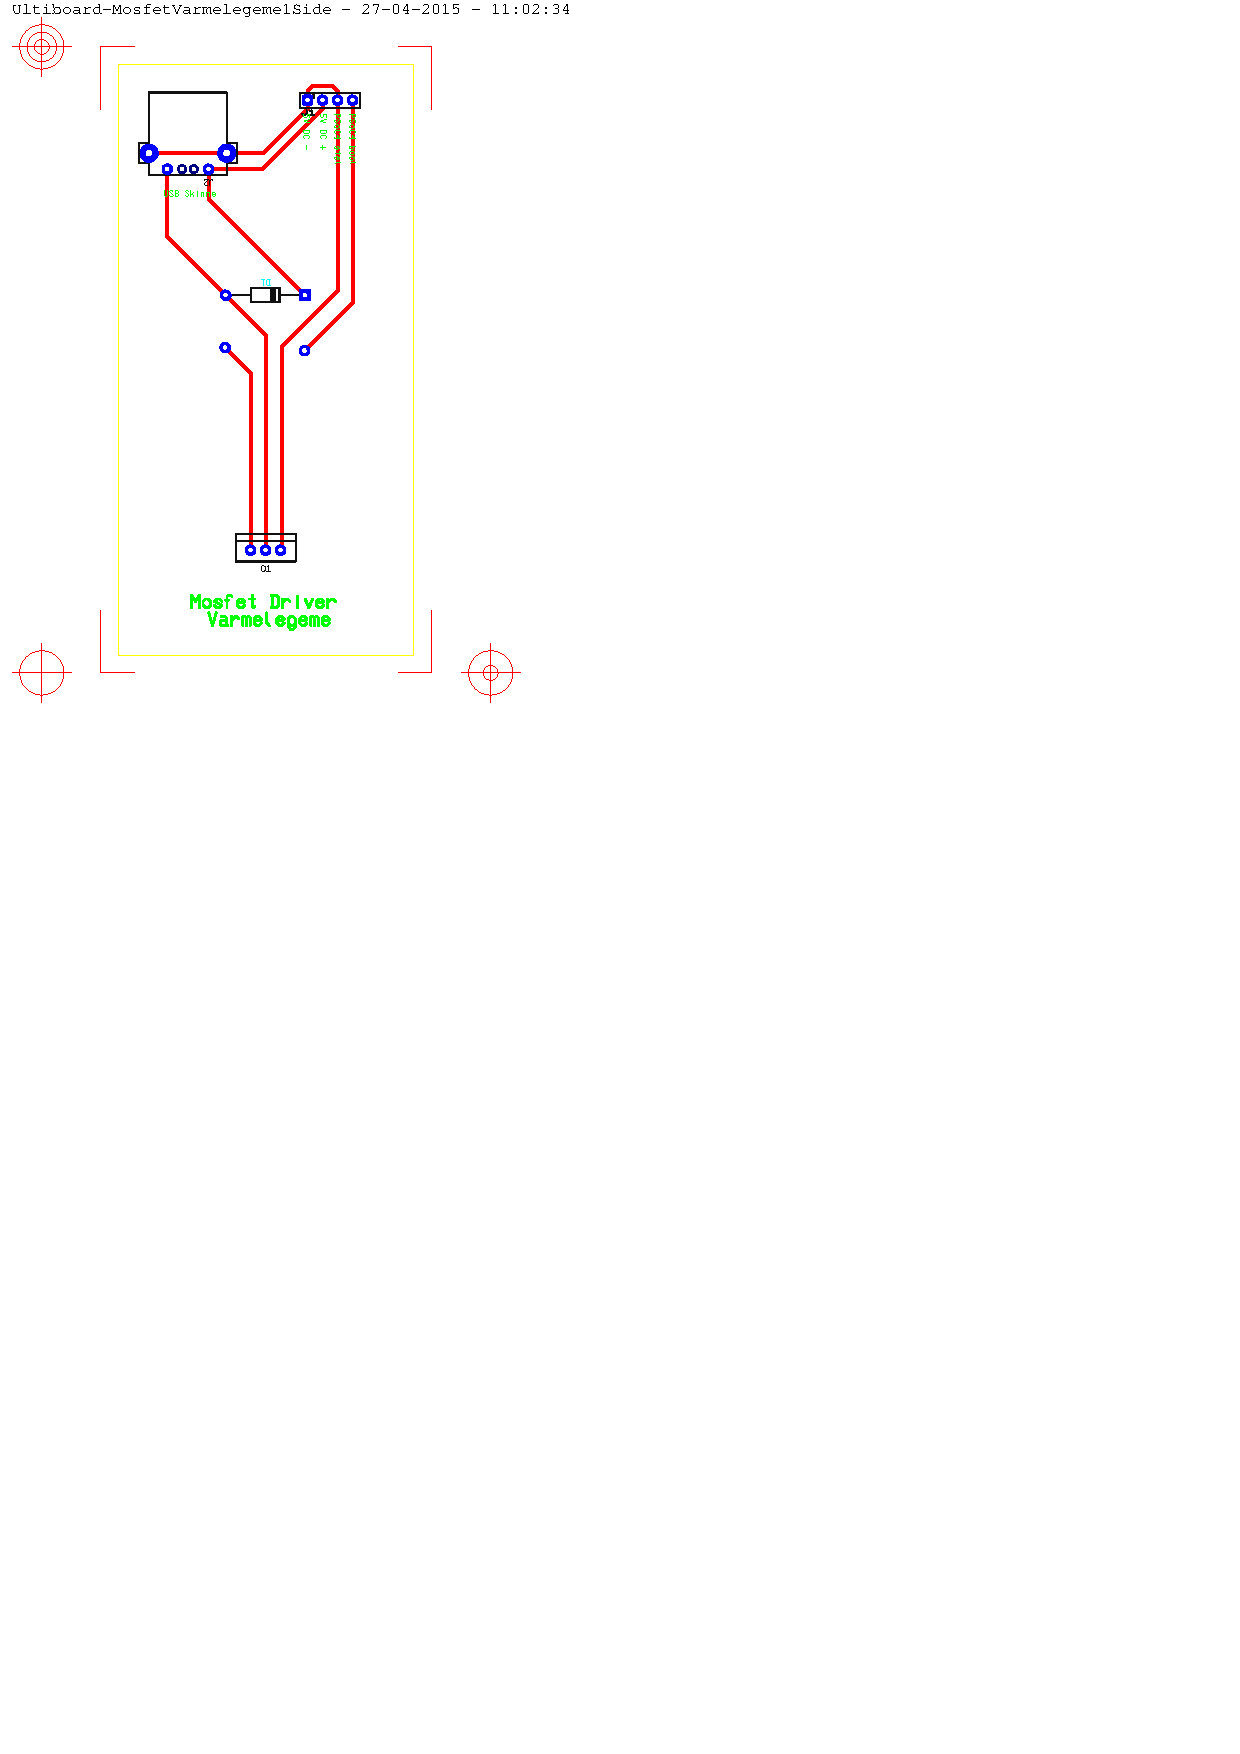
\includegraphics[width={\textwidth-8cm}, trim=50 520 390 30, clip=true, angle =90] {../fig/ultiboard_varmelegeme.pdf}
\caption{Printudlæg for Mosfet driver til Varmelegeme i Ultiboard}
\label{fig:ultiboard_varmelegeme}
\end{figure}

Implementering af mosfet driveren til varmelegemet foretages ved at Multisim diagrammet eksporteres til Ultiboard, hvorefter printet udlægges.
Det forsøges gjort således at printet er overskueligt fremfor at printet fylder så lidt som muligt. 
Som udgangspunkt er alle forbindelser på printet lagt på bagsiden. 
Det designede print er vist på Figur \ref{fig:ultiboard_varmelegeme}. 

Kobber på undersiden af printet er vist med rød, mens kobber på oversiden af printet er vist med grøn. 
Kobberøer er vist med blå.
Der er en lille hage ved kobberøerne; der er ikke forbindelse mellem oversiden og undersiden. 
Dette har dog ingen betydning, da der loddes komponentben igennem dem alle. 

Omkredserne af komponenterne (sort) printes ikke, de vises kun som en slags hjælpelag. 

Databasen i Ultiboard indeholder ikke komponenter til modstande, derfor er disse omkredse ikke med på figuren. 

Der skrives lidt forklarende tekst på oversiden af printet, så man kan se hvad der skal kobles til hvor; dette er lidt svært at se på figuren.
\newline

Printudlægget bestilles ved E-LAB på IHA, hvorefter komponenter loddes på.
Det færdige print er vist på Figur \ref{fig:varmelegeme_print}.

\clearpage

\begin{figure}[h]
\centering 
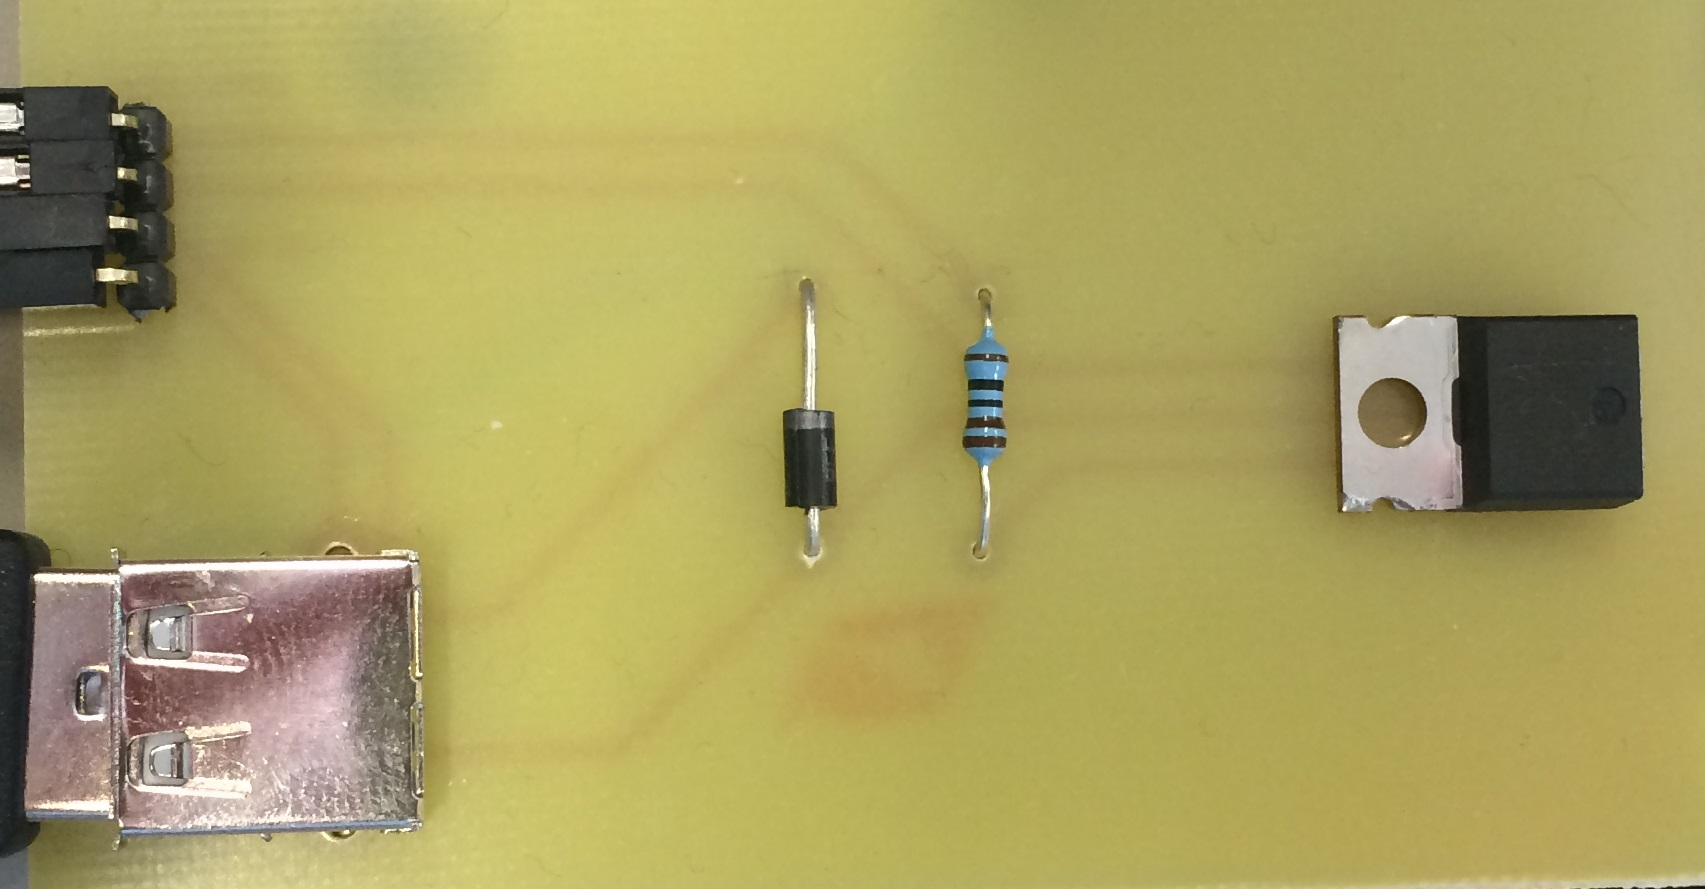
\includegraphics[width={\textwidth-5cm}, trim=0 0 0 0, clip=true] {../fig/VarmePrintBillede} 
\caption{Den færdige Mosfet driver til Varmelegeme}
\label{fig:varmelegeme_print}
\end{figure}

\clearpage

\subsection{HW Blæsere}

Implementering af Mosfetdriver til Blæsere foretages på samme måde som til Varmelegeme.
Printudlægget i Ultiboard er vist på Figur \ref{fig:ultiboard_blaesere}, og det færdige print er vist på Figur \ref{fig:blaesere_print}.

\begin{figure}[h]
\centering 
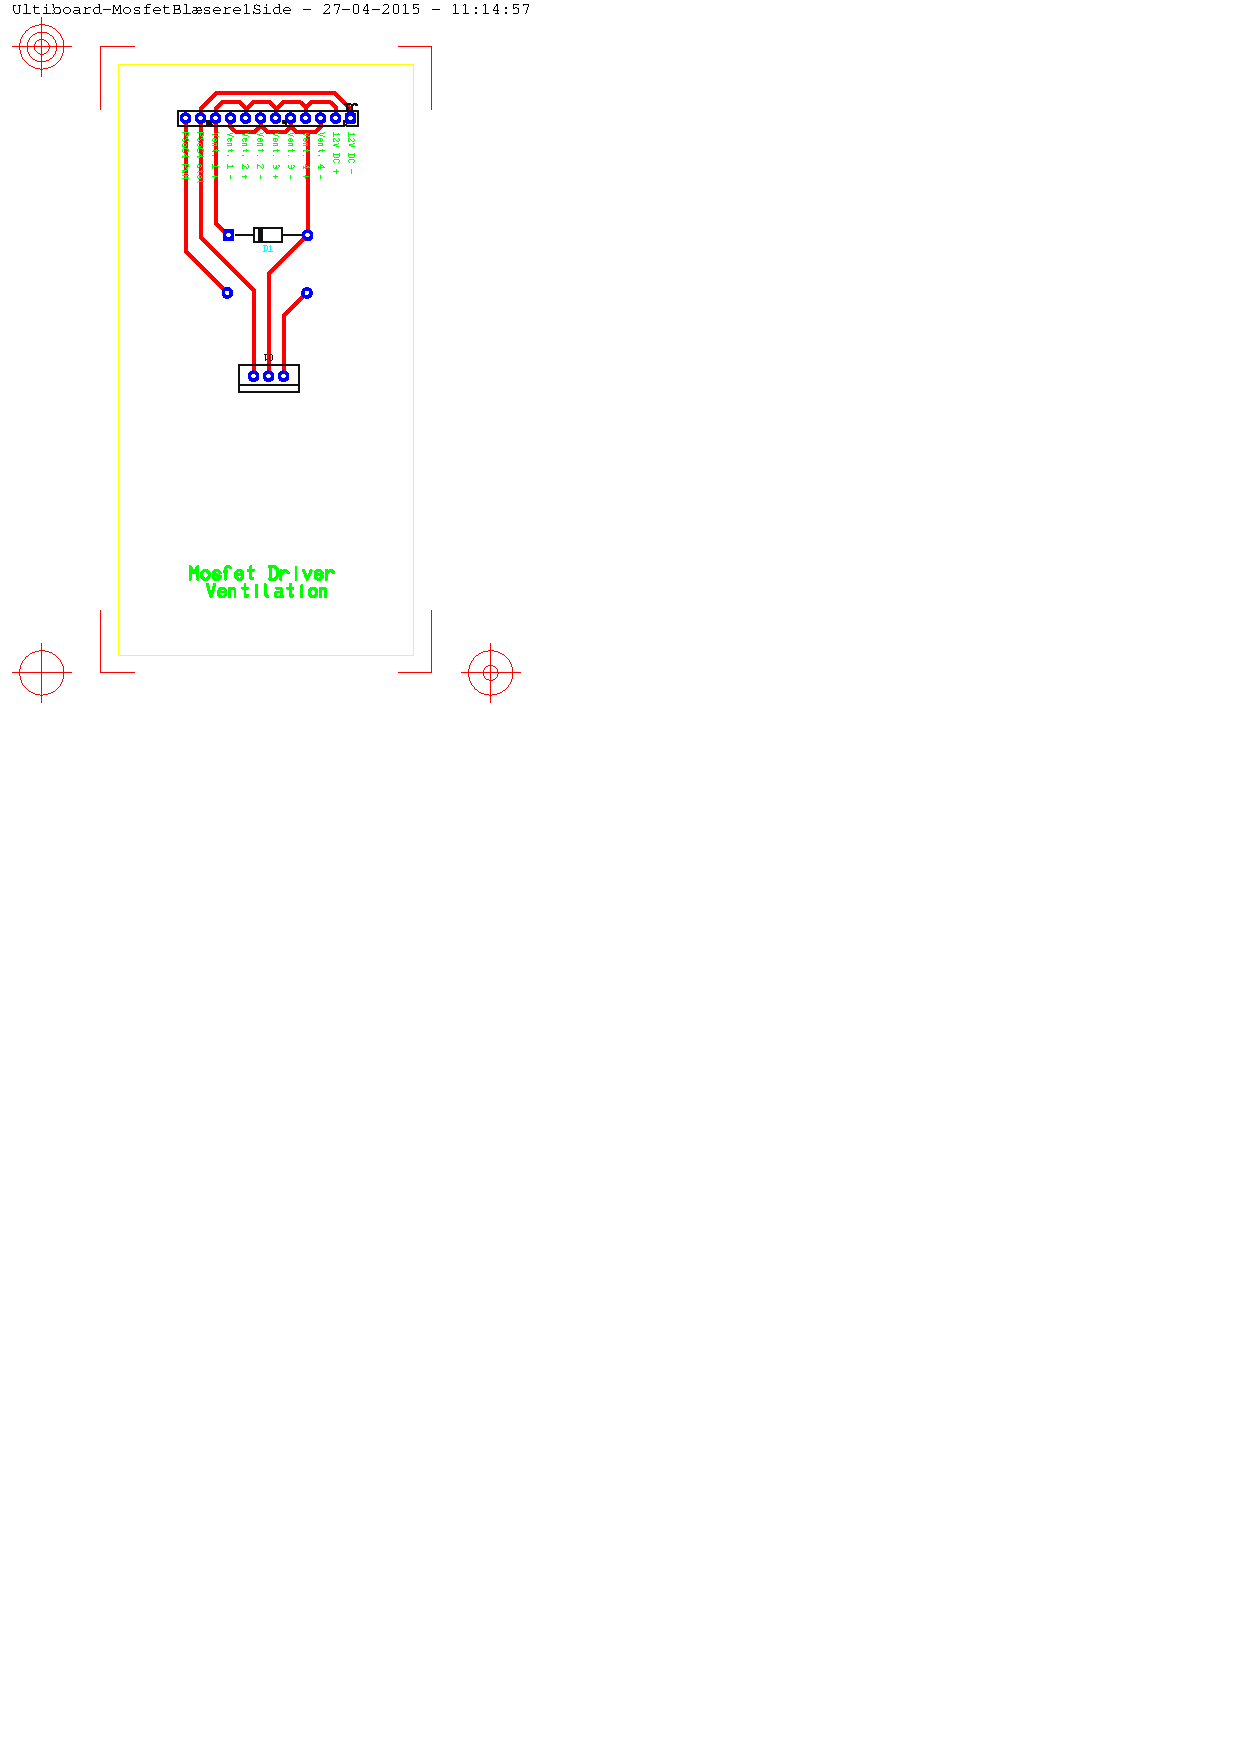
\includegraphics[width={\textwidth-8cm}, trim=50 520 390 30, clip=true, angle =90] {../fig/ultiboard_blaesere.pdf}
\caption{Printudlæg for Mosfet driver til Blæsere i Ultiboard}
\label{fig:ultiboard_blaesere}
\end{figure}

\begin{figure}[h]
\centering 
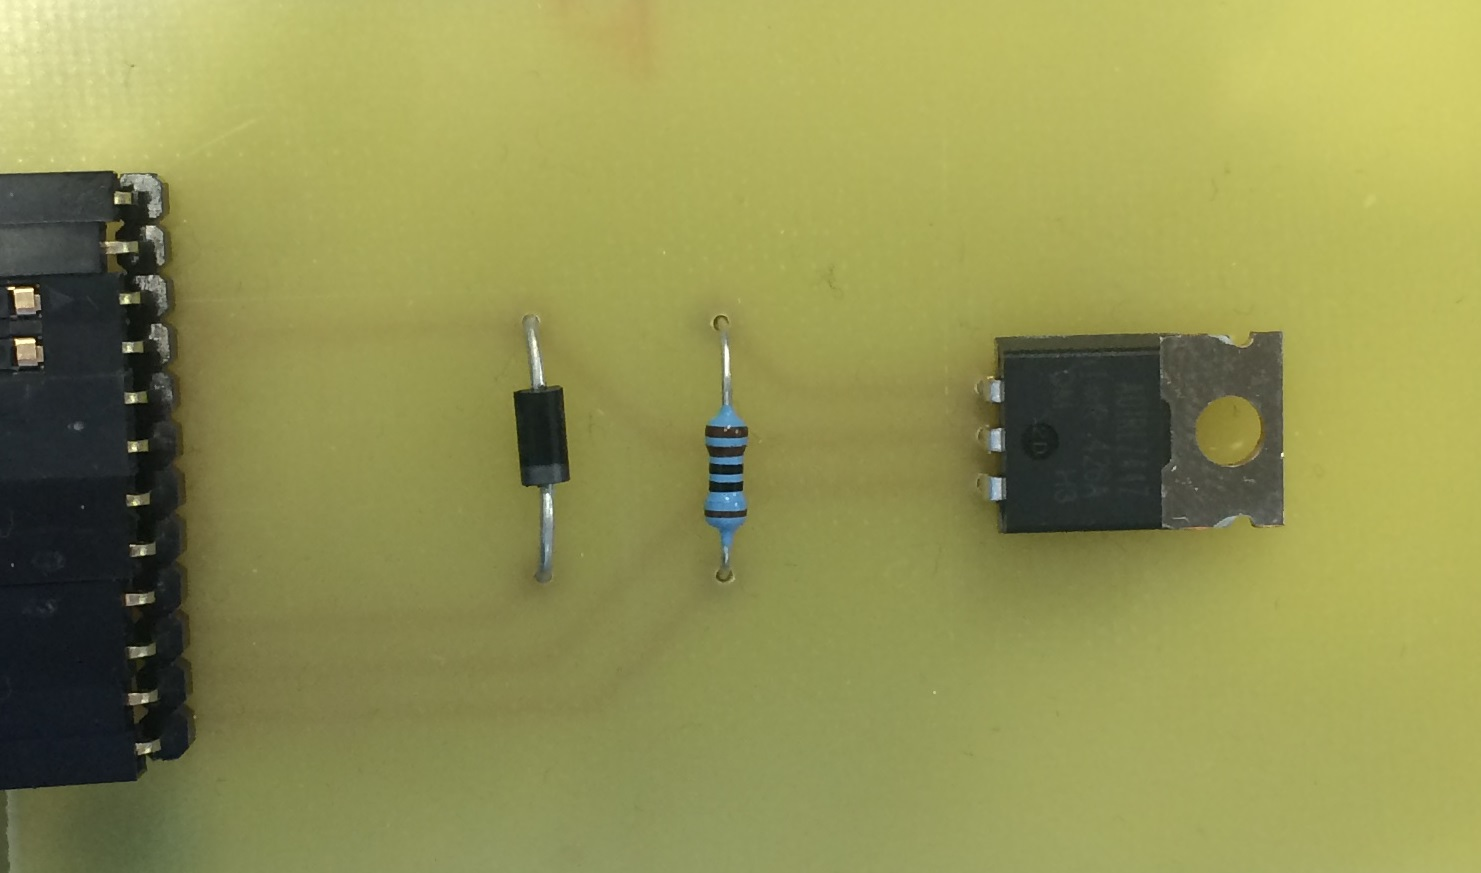
\includegraphics[width={\textwidth-5cm}, trim=0 0 0 0, clip=true] {../fig/VentilationPrintBillede} 
\caption{Den færdige Mosfet driver til Blæsere}
\label{fig:blaesere_print}
\end{figure}

\clearpage

\subsection{HW Vinduesmotor}

Implementering af Mosfetdriver til Vinduesmotor foretages på samme måde som til Varmelegeme og Blæsere.
Printudlægget i Ultiboard er vist på Figur \ref{fig:ultiboard_vinduesmotor}, og det færdige print er vist på Figur \ref{fig:vinduesmotor_print}. 

\begin{figure}[h]
\centering 
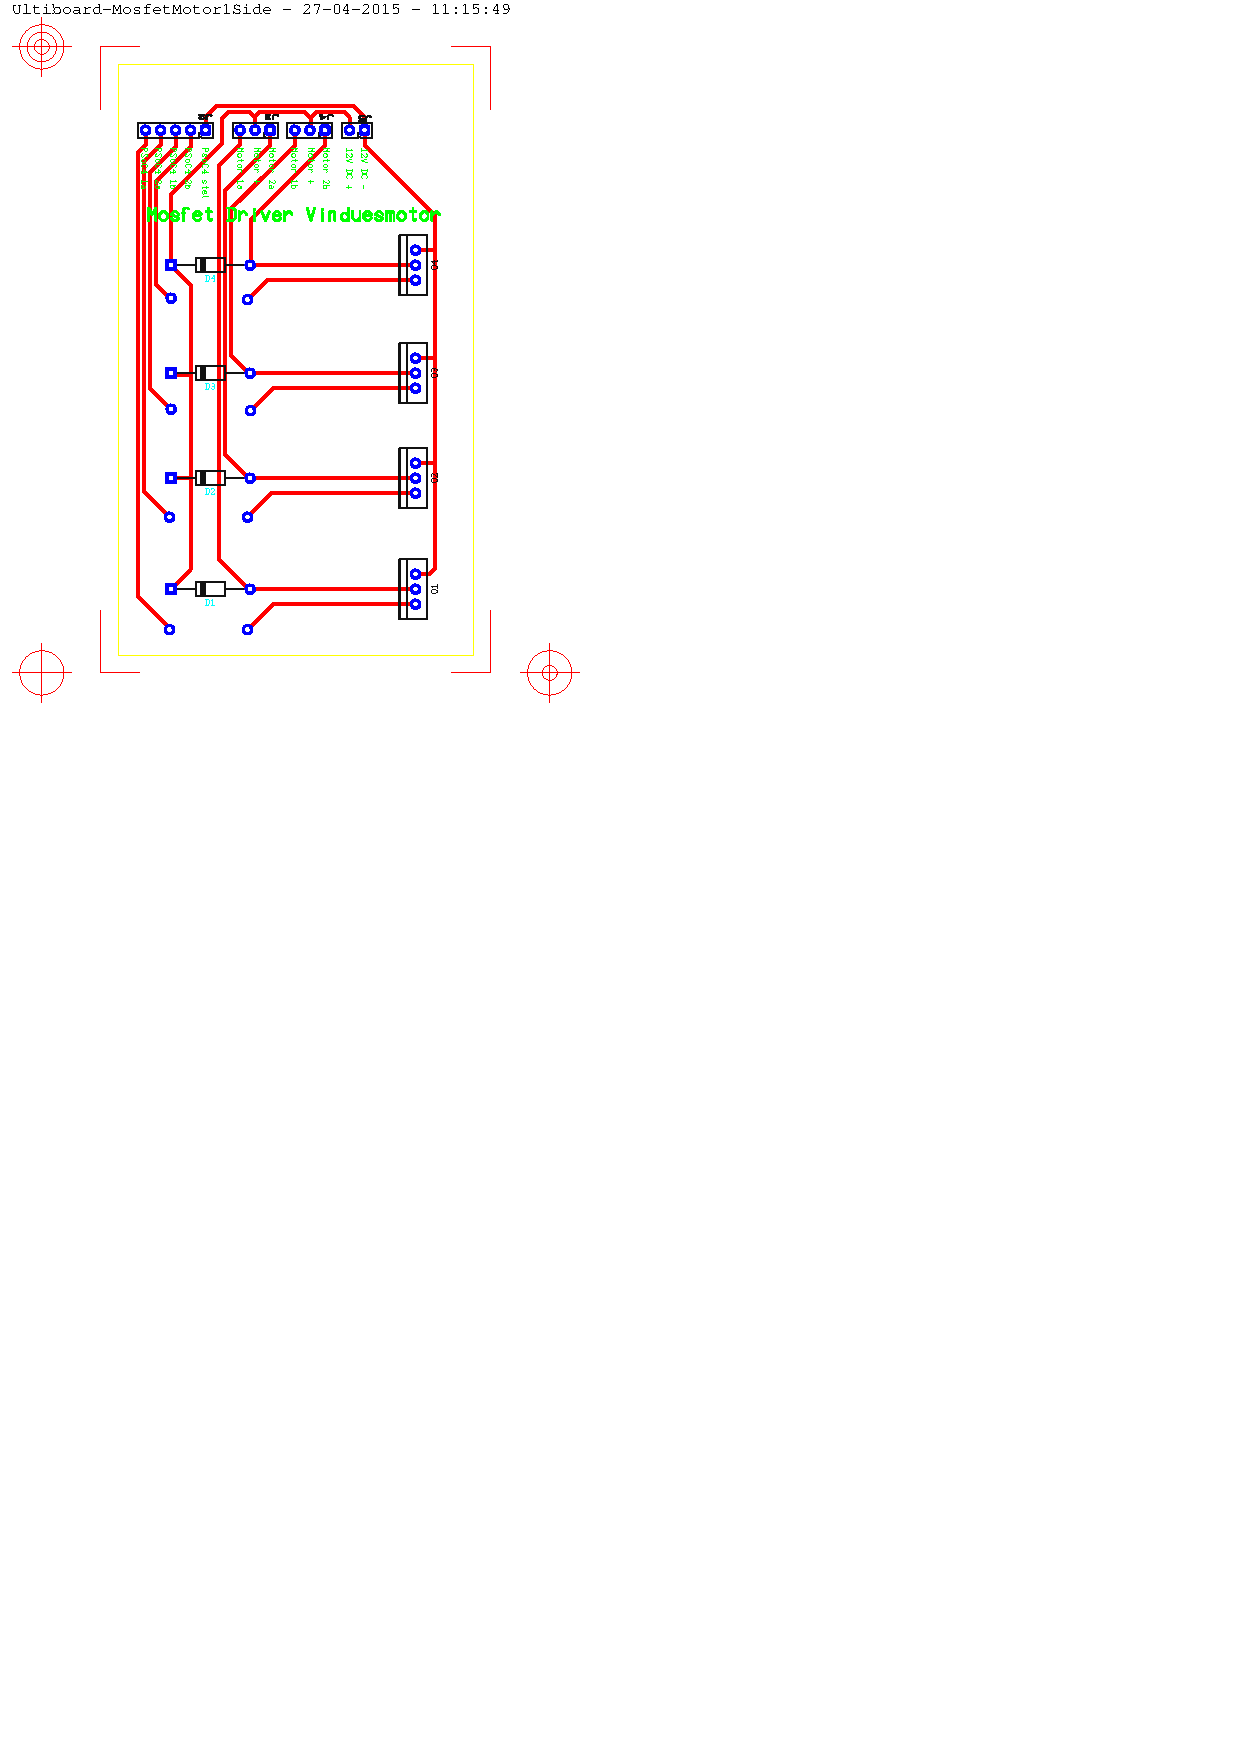
\includegraphics[width={\textwidth-6.5cm}, trim=50 520 365 30, clip=true, angle =90] {../fig/ultiboard_vinduesmotor.pdf}
\caption{Printudlæg for Mosfet driver til Vinduesmotor i Ultiboard}
\label{fig:ultiboard_vinduesmotor}
\end{figure}

\begin{figure}[h]
\centering 
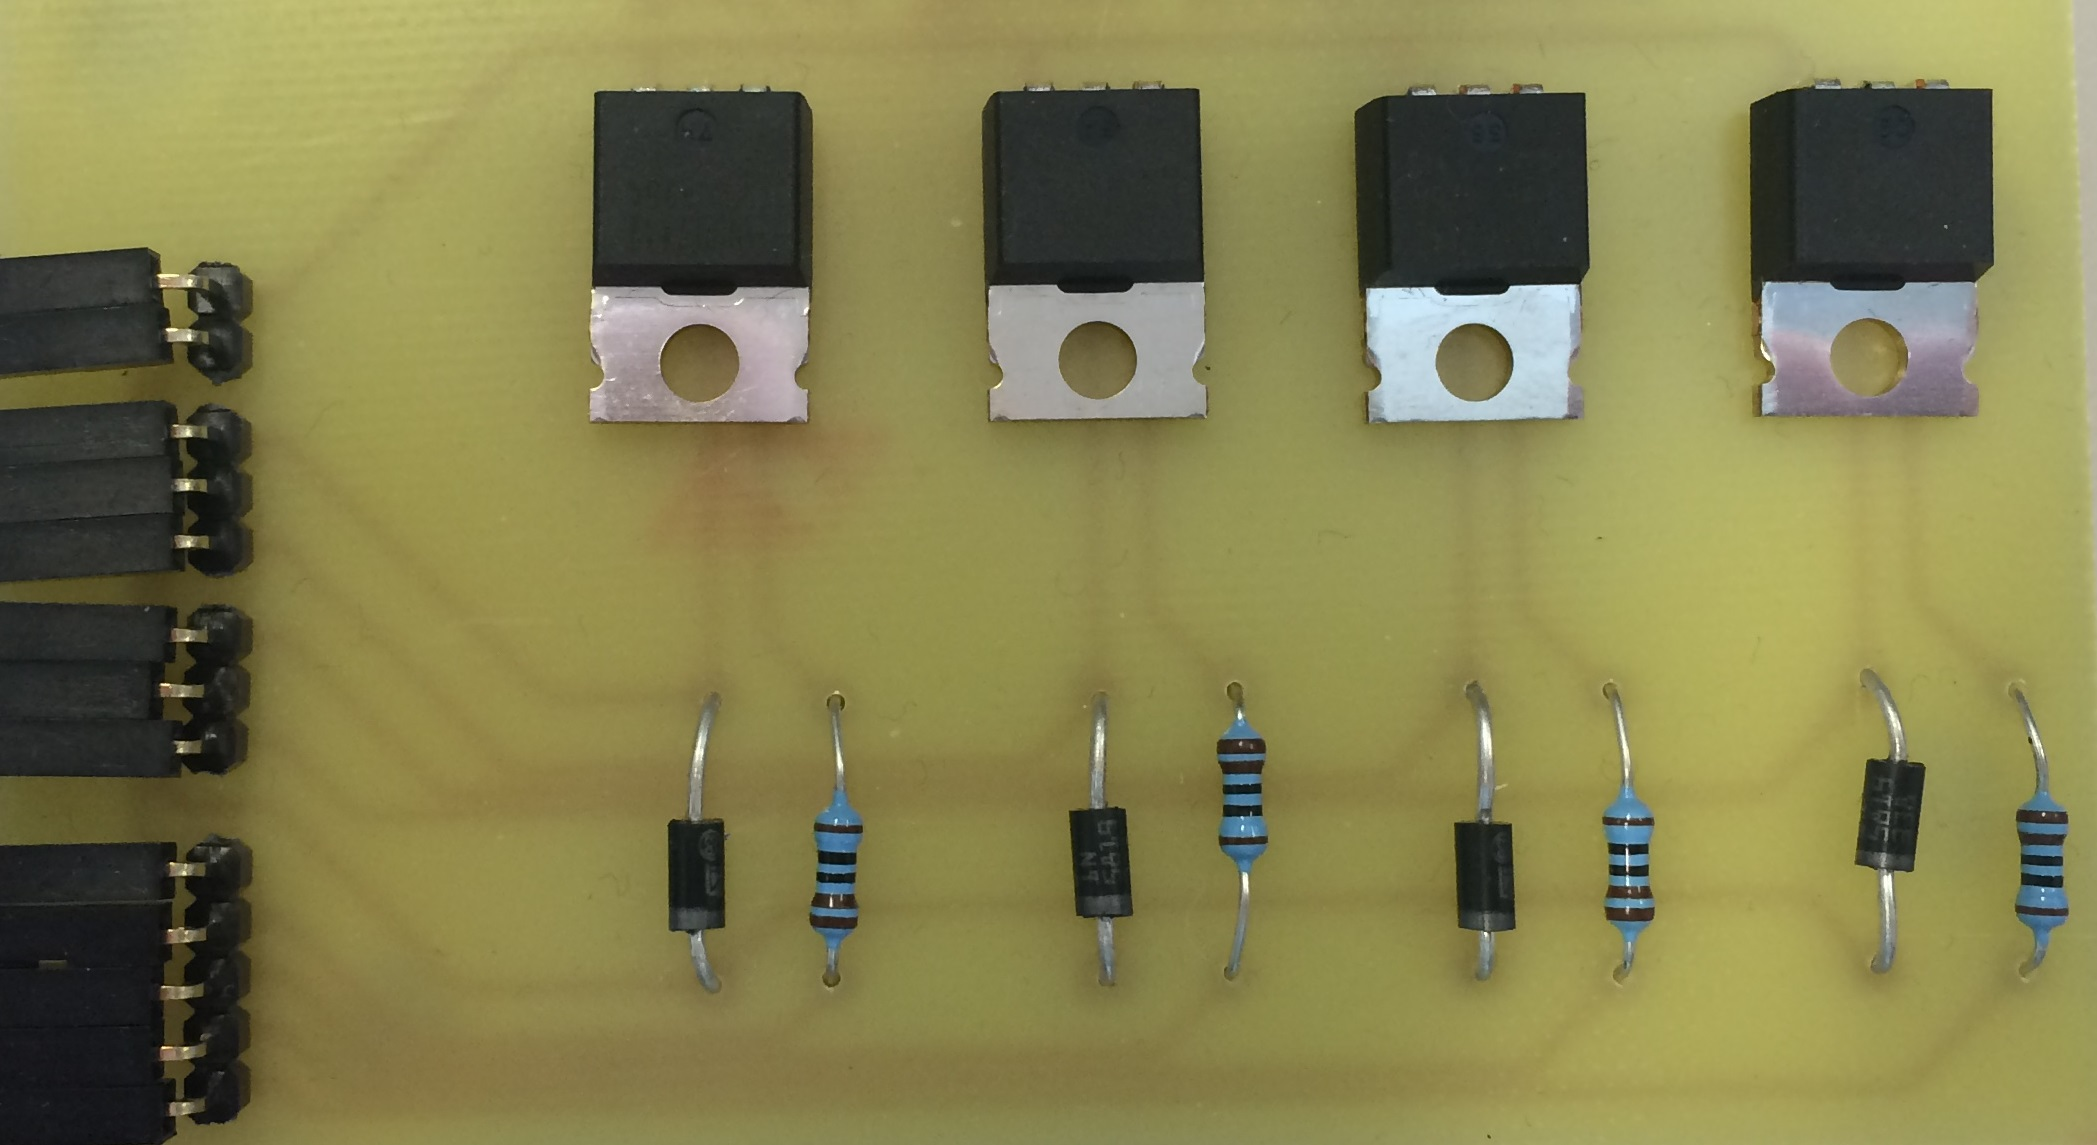
\includegraphics[width={\textwidth-5cm}, trim=0 0 0 0, clip=true] {../fig/MotorPrintBillede} 
\caption{Den færdige Mosfet driver til Vinduesmotor}
\label{fig:vinduesmotor_print}
\end{figure}

\clearpage
\section{PSoC Master implementering} \label{sec:PSoC_Master_impl}

Dette afsnit omhandler overvejelser og det udførte design for PSoC Master blokken i systemet.

\begin{figure}[h]
\centering
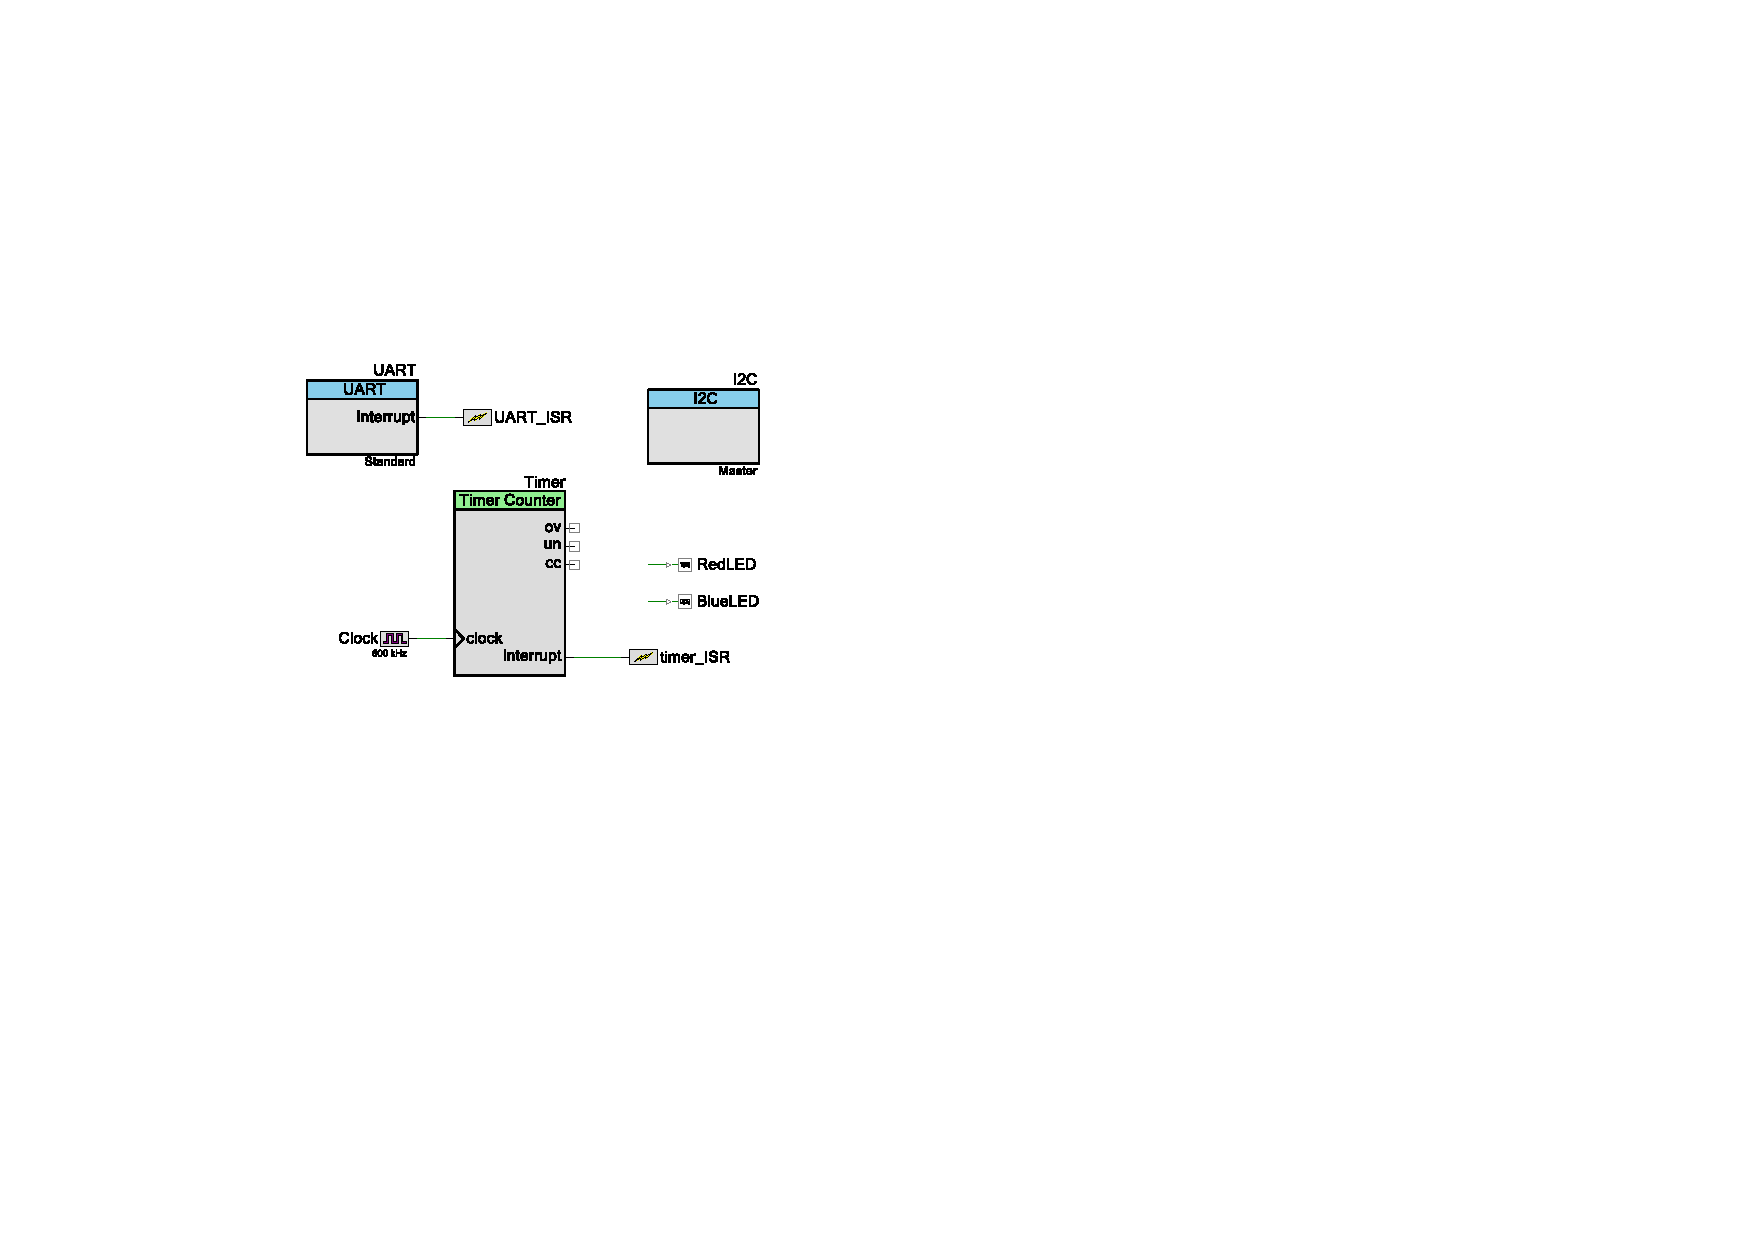
\includegraphics[width=\textwidth*3/5, trim=145 270 475 170, clip=true]{../fig/TopDesign_PSoC_Master}
\label{fig:psoc_master_topdesign}
\caption{TopDesign.cysch for PSoC\_Master}
\end{figure}

I Figur \ref{fig:psoc_master_topdesign} ses topdesignet for PSoC Master. Ud fra dette ses det at vi overordnet set har at gøre med en UART, som genererer interrupts, en Timer, som genererer interrupts, en I2C blok og to outputs til LED. 
Selve topdesignet er lavet ud fra de behov der er stillet i Design-fasen. Der blev under implementeringen af UART overvejet brug af en anden UART komponent, men problemet viste sig at ligge i et tidligere design-valg angående paritet.

\clearpage

\subsection{\IIC implementering}
%TODO Lasse skal kopiere tekst ind her.

\subsection{UART implementering}
UART klassen har til formål at modtage kommandoer fra DevKit8000, tolke disse og give passende svar. 

Generelt set er klassen implementering med udgangspunkt i vores UART protokol, men er udvidet således at der let kan implementeres flere trin i hhv. kontrol af vindue, motor og vanding. UART klassen gør brug af UART komponenten (SCB) vist i Figur \ref{fig:psoc_master_topdesign}.

\begin{lstlisting}[language=C,caption=Implementering af respondTemp(),label=lst:psoc_master_respondTemp]
int8 respondTemp(uint8 temp){
    if(temp){
        // If temp is between 1 and 200(both inclusive) "T" and temp is sent to DevKit8000
        UART_UartPutChar('T');
        UART_UartPutChar(temp);
        return 0;
    }
    else{
        // If temp isn't between 1 and 200(both inclusive) "XT" is sent to DevKit8000
        UART_UartPutChar('X');
        UART_UartPutChar('T');
        return -1;
    }
}
\end{lstlisting}

I Listing \ref{lst:psoc_master_respondTemp} vises et eksempel på en af funktionerne der håndterer svar via UART. De øvrige funktioner i klassen fungerer på samme måde. Funktionen modtager den værdi, der skal sendes tilbage til DevKit8000. Hvis parametren er 0 vil det sige at der er sket en fejl. Når funktionen kaldes kaldes den med returværdi fra DSP klassen, som beskrevet i afsnit \ref{sec:DSP_impl}.

\begin{lstlisting}[language=C, caption=Implementering af dkRequest(), label=lst:psoc_master_dkreq]
uint8 dkRequest(void){
    // Reads the UART buffer
    return UART_UartGetChar();
}
\end{lstlisting}

Vi har ydermere valgt at indkapsle læsningen fra UART ved hjælp af dkRequest() funktionen vist i Listing \ref{lst:psoc_master_dkreq}. 
Grunden til at vi har valgt at implementere denne er for at sikre os at hvis UART protokollen skulle ændre sig i fremtiden, kan disse ændringer tages højde for i denne funktion inden PSoC Master controllerklassen skal håndtere input fra UART.

\subsection{DSP implementering}\label{sec:DSP_impl}
DSP klassen agerer både digital signal processor og domæneklasse for vores måledata. 
Hver type af data er gemt i sit eget array, som vist i Listing \ref{lst:DSP_decl}. 
Hvert arrays har ligeledes en pointer til den næste plads i arrayet der skal overskrives.

\begin{lstlisting}[language=C, label=lst:DSP_decl, caption=Deklaration af arrays og pointers]
// Private data members
int32 tempArray[ARRAYSIZE];
int32* tempArrayPtr;
int32 humArray[ARRAYSIZE];
int32* humArrayPtr;
int16 soilHumArray[NBR_OF_SOILHUM_SENSORS][ARRAYSIZE];
int16* soilHumPtr[NBR_OF_SOILHUM_SENSORS];
int32 lightArray[ARRAYSIZE];
int32* lightArrayPtr;
uint8 temp, hum, soilHum[NBR_OF_SOILHUM_SENSORS], light;     // Used for storing the newest value
\end{lstlisting}



\subsection{Controller implementering}

PSoC\_Master controller-klassen er som udgangspunkt designet ud fra at blive styret af hvilke kommandoer der er modtaget på UART'en. På den måde agerer vores 'master' slave for DevKit8000. 
For at huske den nuværende status er der oprettet en \texttt{enum} med den nuværende status samt ekstra buffer til at holde styr på hvilken vandingsaktuator der modtages data omkring.

\begin{lstlisting}[language=C, label=lst:PSoC_m_dec, caption=Deklaration af buffers og flag.]
// Buffers / flags
typedef enum {IDLE, ADJW, ADJH, ADJV, ADJI} state;
volatile state theState = IDLE;
volatile int8 irrigationIndex = 0;
uint8 newByte = 0;
uint8 buff;
\end{lstlisting}

Ydermere er der lavet en form for debugging ved hjælp af de tre farvede LED'er på PSoC4 Pioneer Kit. Der tændes fx for den røde LED når et interrupt sker på timeren og for den blå når et interrupt sker på UARTen.

Når der sker et interrupt på UART'en, sættes flaget \texttt{newByte} til 1 og der fyldes data i bufferen. Dette ses i Listing \ref{lst:PSoC_m_uart_int}.

\begin{lstlisting}[language=C, label=lst:PSoC_m_uart_int, caption=ISR for UART.]
// UART ISR
CY_ISR(UART_ISR){
    newByte = 1;
    buff = dkRequest();
    UART_ClearRxInterruptSource(UART_GetRxInterruptSourceMasked());     // Clear interrupt flag
}
\end{lstlisting}

Årsagen til at vi har valgt at sætte et flag er at vi hurtigst muligt vil ud af interrupt service rutinen samt at det gav os problemer at have al funktionaliteten som kald fra UART ISR.

Der er herefter udarbejdet en ny privat funktion kaldet \texttt{uartIntHandler()},  %TODO Opdater navnet på inthandler
som sørger for at håndtere selve arbejdet mht. det input UART'en giver. 
Denne bliver kaldt med jævne mellemrum fra en \texttt{while(1)} løkke i main.c. 

\begin{lstlisting}[language=C, label=lst:PSoC_m_uartinth, caption=Interrupt handler for UART.]
void intHandler(){
    if (newByte){
        newByte = 0;
        BlueLED_Write(LED_ON);       // Turn on blue LED
        
        if(theState == IDLE){
            switch (buff){
                case 'T':{ //RequestTemp
                    respondTemp(getTemp_DSP());		
                    break;
                }
                case 'L':{ //RequestLight
                    respondLight(getLight_DSP());
                    break;
                }
                case 'A':{ //RequestAirhum
                    respondHum(getHum_DSP());
                    break;
                }        
                case 'H':{ //TurnHeatOn
                    // 0x7 is the maximum value.
                    respondHeat(adjustHeat(0x7), 'H');
                    break;
                }
                case 'K':{ //TurnHeatOff
                    // 0x0 is the minimum value.
                    respondHeat(adjustHeat(0x0), 'K');
                    break;
                }
                case 'W':{ //AdjustWindow
                    theState = ADJW;
                    break;
                }
                case 'V':{ //Ventilation
                    theState = ADJV;
                    break;
                }
                case 'F':{ //Watering
                    theState = ADJI;
                    break;
                }
                /*case 'S':{ //
                    respondSoilHum(); //TODO: Add stuff here
                    break;
                }*/
                default:{
                    // Do nothing - let the DevKit8000 timeout
                    break;
                }
            }
        }
        else if(theState == ADJW){
            if(buff-CONVERT_TO_ASCII == 1){
                respondWin(adjustWindow(0xFF));
            }
            else{
                respondWin(adjustWindow(0x00));
            }
            theState = IDLE;
        }
        else if(theState == ADJV){
            if(buff-CONVERT_TO_ASCII == 1){
                respondVent(adjustVentilation(0xFF));
            }
            else{
                respondVent(adjustVentilation(0x00));
            }
            theState = IDLE;
        }
        else if(theState == ADJI){
            if (!irrigationIndex){
                irrigationIndex = buff;
            }
            else{
                if (buff-CONVERT_TO_ASCII == 1){
                    respondIrri(adjustIrrigation(irrigationIndex-CONVERT_TO_ASCII-1, 0xFF));
                }
                else{
                    respondIrri(adjustIrrigation(irrigationIndex-CONVERT_TO_ASCII-1, 0x00));
                }
                irrigationIndex = 0;
                theState = IDLE;
            }
        }
        buff = 0;
        BlueLED_Write(LED_OFF);         // Turn off blue LED
    }
}
\end{lstlisting}

I Listing \ref{lst:PSoC_m_uartinth} ses implementeringen af selve interrupthandleren. Det ses hvordan der først tjekkes for om der er kommet ny data via \texttt{newByte} og der herefter kontrolleres hvilket stadie, systemet er i. Hvis det er i \texttt{IDLE} tjekkes der på hvad der står i bufferen og der udfærdes evt et svar eller ventes på næste databyte. Til at starte med tændes den blå LED og når kaldet er slut slukkes denne.

\clearpage %TODO When done, uncomment this line!
%TODO SoftwareImpl?
%TODO Konklusion?
\renewcommand{\bibname}{Litteraturliste}
\fancyhead[CE,CO]{}
\fancyfoot[CE,CO]{}
\begin{thebibliography}{2}

\bibitem {lib:DK8000} Timll Technic Inc: \textit{DevKit8000 brugermanual}. \\ 
"Bilag 001 - DevKit8000 User Manual En". 2009.

\bibitem {lib:psoc4_guide} Cypress Semiconductor: \textit{PSoC 4 Pioneer Kit Guide}. \\
"Bilag 002 - CY8CKIT-042 PSoC 4 Pioneer Kit Guide". 2013.

\bibitem {lib:TempHum_DS} Honeywell International Inc.: \textit{Datablad for Temperatur-/Luftfugtighedssensor}. \\
"Bilag 003 - Datablad for Temp og Luftfugtsensor". August 2013.

\bibitem {lib:TempHum_I2C} Honeywell International Inc.: \textit{\IIC Communication with the Honeywell HumidIcon}. \\
"Bilag 004 - I2C Communication with the Honeywell HumidIcon". June 2012.

\bibitem {lib:LightSens} Intersil: \textit{Datablad for lyssensor}. \\
"Bilag 005 - Datablad for lyssensor". Februar 2008.

\bibitem {lib:LM7805_DS} Motorola, Inc.: \textit{Three-Terminal Positive Voltage Regulators}. \\
"Bilag 006 - Datablad for LM7805". Maj 1996.

\bibitem {lib:UHD2_DS} SAIA-Burgess Electronics: \textit{Motor Products}. \\
"Bilag 007 - Motor Products". 2000.

\bibitem {lib:LM75} Maxim: \textit{Digital Temperature Sensor and Thermal
Watchdog with 2-Wire Interface}. \\
"Bilag 008 - Datablad for LM75". 2009.

\bibitem {lib:MSE_06} PRJ3 F15 Gruppe 9: \textit{MSE Øvelse 6}. \\
"Bilag 009 - MSE Øvelse 6". Maj 2015. 

\bibitem {lib:USB20} USB Implementers Forum, Inc.: \textit{USB 2.0 Specification}.\\
\url{http://www.usb.org/developers/docs/usb20_docs/#usb20spec}. Marts 2015.

\bibitem {lib:PSoC_m_git} PRJ3 F15 Gruppe 9: \textit{PSoC Master source code}. \\
\url{https://github.com/PhKP/PSoC_Master}. 2015.

\bibitem {lib:DevKit8000_Addon} Devkit8000 wiki, IHA: \textit{DevKit8000 wiki}. \\
\url{https://redmine.iha.dk/devs/projects/devkit8000/wiki/Addon_board}. Dec 2013.

\bibitem {lib:UART_opensource} Beelen, Teunis van: \textit{RS232 UART-protokol}. \\
\url{http://www.teuniz.net/RS-232/} . Jan 2015.

\bibitem {lib:threadconcept} Codebase.eu: \textit{Multithreading}. \\
\url{http://codebase.eu/tutorial/posix-threads-c/}. Sep 2011

\bibitem {lib:QT} The QT company: \textit{QT info}. \\
\url{http://doc.qt.io/qt-4.8/timers.html}. Feb 2015.

\bibitem {lib:Event_driven_programming} Wikipedia: \textit{Event Driven Programming}. \\
\url{http://en.wikipedia.org/wiki/Event-driven_programming}. Maj 2015.

\bibitem {lib:multi_threading} The Open Group. \textit{Multi threading}. \\
\url{http://pubs.opengroup.org/onlinepubs/9699919799/basedefs/pthread.h.html}. 2013.

\end{thebibliography}
%etc...

\end{document}